\documentclass[12pt, a4paper]{report}

% --- Paquetes básicos ---
\usepackage[utf8]{inputenc}
\usepackage[T2A,T1]{fontenc}
\usepackage[spanish]{babel}
\usepackage{amsmath}
\usepackage{amssymb}
\usepackage{amsfonts}
\usepackage{amsthm}
\usepackage{geometry}
\usepackage{mathtools}
\usepackage{epigraph}
\usepackage{enumitem}
\usepackage{stmaryrd}
\usepackage{comment}
\usepackage{graphicx} % <--- AGREGADO: Necesario para la imagen uba2.jpg
\usepackage[colorlinks=true, linkcolor=blue]{hyperref}
\usepackage{tikz}
\usetikzlibrary{babel,positioning,arrows.meta,calc}

% --- Configuración de márgenes GENERAL (para el resto de la tesis) ---
\geometry{left=3cm, right=3cm, top=3cm, bottom=3cm}
% --- Configuración de entornos de Teoremas/Definiciones ---
\theoremstyle{definition}
\newtheorem{definition}{Definición}[section]
\newtheorem*{definition*}{Definición}
\newtheorem{example}[definition]{Ejemplo}
\newtheorem*{example*}{Ejemplo}
\newtheorem{remark}[definition]{Observación}
\newtheorem{recordatorio}[definition]{Recordatorio}
\newtheorem{conjecture}[definition]{Conjetura}

\theoremstyle{plain}
\newtheorem{theorem}[definition]{Teorema}
\newtheorem*{theorem*}{Teorema}
\newtheorem{lemma}[definition]{Lema}
\newtheorem*{lemma*}{Lema}
\newtheorem{prop}[definition]{Proposición}
\newtheorem*{prop*}{Proposición}
\newtheorem{corollary}[definition]{Corolario}
\newtheorem*{corollary*}{Corolario}

\renewcommand{\proofname}{Demostración}

% --- Comandos personalizados ---
\DeclareMathOperator{\SL}{SL}
\DeclareMathOperator{\GL}{GL}
\DeclareMathOperator{\im}{Im}
\DeclareMathOperator{\ord}{ord}
\DeclareMathOperator{\nuord}{\nu}
\DeclareMathOperator{\mcd}{mcd}
\newcommand{\Hcal}{\mathbb{H}}
\newcommand{\CC}{\mathbb{C}}
\newcommand{\RR}{\mathbb{R}}
\newcommand{\QQ}{\mathbb{Q}}
\newcommand{\ZZ}{\mathbb{Z}}
\newcommand{\FF}{\mathbb{F}}
\newcommand{\NN}{\mathbb{N}}
\newcommand{\PP}{\mathbb{P}}
\newcommand{\OO}{\mathcal{O}}
\newcommand{\cc}{\mathcal{C}}
\newcommand{\ee}{\mathcal{E}}
\newcommand{\pp}{\mathfrak{p}}
\newcommand{\aaa}{\mathfrak{a}}

\newcommand{\Sha}{\text{\fontencoding{T2A}\selectfont\CYRSH}}

\newcommand{\QmodD}{\QQ^\times / {(\QQ^\times)}^2}
\newcommand{\QmodT}{\QQ^\times / {(\QQ^\times)}^3}
\newcommand{\QmodN}{\QQ^\times / {(\QQ^\times)}^n}
\newcommand{\KmodD}{K^\times / {(K^\times)}^2}
\newcommand{\KmodT}{K^\times / {(K^\times)}^3}
\newcommand{\KmodN}{K^\times / {(K^\times)}^n}

\newcommand{\mat}[4]{\begin{pmatrix} #1 & #2 \\ #3 & #4 \end{pmatrix}}
\newcommand{\minmat}[4]{\left(\begin{smallmatrix} #1 & #2 \\ #3 & #4 \end{smallmatrix}\right)}
\newcommand{\qexp}{e^{2\pi i z}}
\newcommand{\leg}[2]{\left(\frac{#1}{#2}\right)}
\newcommand{\cub}[2]{\left(\frac{#1}{#2}\right)_3}

\newcommand{\lp}{\left(}
\newcommand{\rp}{\right)}
\newcommand{\lb}{\left|}
\newcommand{\rb}{\right|}
\newcommand{\lc}{\left<}
\newcommand{\rc}{\right>}
\newcommand{\lco}{\left[}
\newcommand{\rco}{\right]}
\newcommand{\lla}{\left\{}
\newcommand{\rla}{\right\}}


% --- Configuración de hyperref ---
\hypersetup{
    colorlinks=true, linkcolor=blue, citecolor=magenta, urlcolor=cyan
}

% --- Inicio del Documento ---
\begin{document}

% --- CARÁTULA PERSONALIZADA ---
\begin{titlepage}
    % Cambiamos los márgenes SOLO para esta página según pide la plantilla de UBA
    \newgeometry{top=5cm, bottom=2cm, left=3cm, right=3cm}
    
    \thispagestyle{empty}

    \begin{center}
        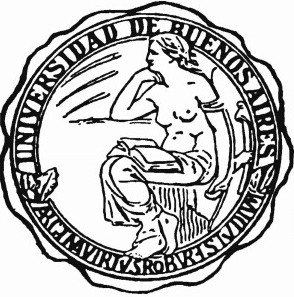
\includegraphics[scale=.3]{uba2.jpg}

        \medskip
        \textbf{UNIVERSIDAD DE BUENOS AIRES}

        \smallskip 

        \textbf{Facultad de Ciencias Exactas y Naturales}

        \smallskip

        \textbf{Departamento de Matem\'atica}

        \vspace{3.5cm}

        \textbf{\large Tesis de Licenciatura}

        \vspace{1.5cm}

        \textbf{\large Como construir infinitas curvas elipticas con un rango fijo.}

        \vspace{1.5cm}

        \textbf{Pedro Nicolás Peña}

    \end{center}

    \vspace{1.5cm}

    \noindent \textbf{Director} \ \ Dr. Martin Mereb

    \vspace{3cm}

    \rightline{\today}

    % Restauramos los márgenes globales (3cm) para el resto del documento
    \restoregeometry
\end{titlepage}
% --- FIN CARÁTULA ---

\newpage
\clearpage
\newpage

\section*{Agradecimientos}

A Juli Feldman que me paso este template.



\newpage

\section*{Introducción}

El objetivo de esta tesis es recopilar la teoria necesaria para la construccion de ejemplos de familias de curvas elipticas de un rango fijo, junto con todos los nuevos metodos que vayan se vayan incorporando en aplicaciones al area. Sobre este tema han habido recientes avances que combinan ideas y desarrollos previos en un resultado novedoso. Este documento se irá actualizando conforme avance el área como un resumen de los metodos que surjan, las nuevas versiones se encontraran en el GitHub de su autor.

El grupo abeliano de puntos racionales de una curva eliptica $E$ sobre un cuerpo de números $K$ es finitamente generado, y podemos considerar su parte de torsion y el rango de su parte libre. 

Nos enfocaremos en el rango, que es un valor del que se sabe mucho menos que la torsion, y es componente de muchas conjeturas famosas. De las preguntas principales sobre él algunas son: el rango maximo que puede alcanzar una curva definida sobre $\QQ$, con el record actual de rango al menos $31$ por Alpöge y Howell~\cite{DujellaRankRecords}, o el maximo dado un grupo de torsion fijo, ver~\cite{ElkiesKlagsbrun2020}; que valores de rango aparecen infinitas veces, con una heuristica por Park, Poonen, Voight y Wood~\cite{ParkPoonenVoightWood2019} que predice infinitas curvas de cada rango hasta $20$ y solo finitas de rango mayor que $21$, dejando abierto el caso $21$; muchas conjeturas que lo relacionan con otros invariantes de la curva, siendo la mas famosa la de Birch y Swinnerton-Dyer; y la de dar familias \emph{explicitas} de curvas de un rango fijo, que recien en el ultimo tiempo se comenzaron a obtener ejemplos gracias a una inteligente combinacion de resultados ya conocidos. Hay tambien resultados de densidad, como el de Bhargava y Shankar que nos dice que el rango promedio es menor a $3/2$, cota que se fue mejorando.

Un resultado conocido de Silverman nos da una forma de construir infinitas curvas sobre $\QQ$ de rango al menos $r$ via especializaciones de una curva eliptica definida sobre $\QQ(T)$. Usando el metodo del descenso, que se usaba en casos particulares, junto con resultados de combinatoria aditiva para aplicarlo en toda una familia, se logró encontrar una forma de acotar superiormente el rango. Logrando que la cota superior sea igual a la inferior obtenemos una familia de curvas de un rango fijo. El mejor resultado hasta la fecha es el de Zywina~\cite{Zywina2026SmallRank} que da ejemplos de curvas de rango $r$ para todo $0\leq r \leq 4$ y para todo cuerpo de numeros $K$. 

Tambien surge el interes de resultados analogos fijando cierta condicion para la curva, y en nuestro caso lo haremos con el $j$-invariante. Los valores que tienen un comportamiento diferente son $j=1728$, naturalmente interesante sobre $\QQ(i)$, para el cual Savoie~\cite{Savoie2025QiRank2} dio una familia de curvas de rango 2; y $j=0$ sobre $\QQ(\omega)$, que estudiaremos aqui.


\subsection*{Estructura de la tesis y notacion}

La estructura de la tesis será la siguiente: en el capitulo 1 reuniremos resultados generales sobre curvas elipticas que vayamos a usar mas adelante; el capitulo 2 presenta las herramientas que nos permiten obtener un minimo para el rango, que son las superficies elipticas o K3 y los teoremas de especializacion para bajar a curvas elipticas; el tercero se encarga de la cota superior, junto con el desarrollo de la teoria para hacerla computable y ejemplos; en el cuarto incluiremos resultados de distribucion de primos, que provienen de otro area y por lo tanto usaremos como ``caja negra'', pero que son principales para la generacion de infinitos ejemplos que cumplan nuestras condiciones; y finalmente en el ultimo capitulo reuniremos las aplicaciones, con desarrollos que se fueron presentando como ejemplos a lo largo de la tesis, para presentar un resultado nuevo. Cada capitulo tiene una recapitulacion donde se pueden encontrar la teoria del mismo pero concentrada como para su aplicacion directa al problema que nos interesa. 

Antes de empezar fijemos la notacion que usaremos. A lo largo de la tesis trabajaremos mayormente con cuerpos de numeros (extensiones finitas de $\QQ$) y los denotaremos $K$; y, aunque muchos resultados se pueden extender a cuerpos arbitrarios, otros tantos no, y no haremos mencion en cada caso. El grupo de puntos de una curva eliptica $E$ sobre $K$, por ser un grupo abeliano finitamente generado, lo escribiremos
\[
E(K)\cong T\oplus\ZZ^r,
\]
donde $T$ es el grupo de torsion y $r=\operatorname{rg}E(K)$ es el rango.

Usaremos la notacion habitual de teoria de numeros algebraica, que resumimos a continuacion: Denotaremos $\OO_K$ al anillo de enteros, $\bar K$ a una clausura algebraica y $G_K=\operatorname{Gal}(\bar K/K)$. El grupo $E[n]$ contiene todos los puntos anulados por $[n]$ sobre $\bar K$, mientras que $E(K)[n]$ contiene solo los definidos sobre $K$; la misma convencion vale para cualquier isogenia $\phi$. Los lugares de $K$ forman el conjunto $M_K$. Para un lugar $v$, $K_v$ es la completacion respecto a la valuacion de $v$; si es finito y corresponde al ideal primo $\pp$, tambien escribiremos $K_\pp$ y usaremos la valuacion $v_\pp$, con $v_\pp(0)=+\infty$.

Para nuestro caso particular de interes fijamos $\omega=(-1+\sqrt{-3})/2$, de modo que $\omega^2+\omega+1=0$. Usaremos una curva en especifico, pero la iremos presentando con mas o menos generalidad para simplificar la notacion. $E_d:y^2=x^3+d$ será la mas general, llamada curva de Mordell; luego, para asegurarnos el punto de 3-torsion $(0,t)$, tomaremos $d=t^2$ y la llamaremos $E_t:y^2=x^3+t^2$; despues usaremos $t=k^2-1$, con el cual tenemos un punto libre sobre el cuerpo de funciones, y la curva será $E_k:y^2=x^3+(k^2-1)^2$; finalmente escribiremos $k=a/b$ y, tras el cambio $(x,y)\mapsto(b^2x,b^3y)$, tendremos
\[
E_{a,b}:y^2=x^3+{\lp b(a-b)(a+b)\rp}^2.
\]
El subindice indica la parametrizacion que estamos usando, siempre con coeficiente no nulo. 

\newpage
\tableofcontents
\newpage


\chapter{Preliminares: curvas elipticas y grupo de Mordell-Weil}\label{cap:mw}

\section{Motivacion}\label{sec:motivacion}

Una ecuacion diofantica es una ecuacion polinomial de la que buscamos soluciones enteras o racionales. Esto en general nos interesa porque pueden modelar problemas que nos interesen. Veamos algunos ejemplos:
\begin{itemize}
    \item Pedir que el producto de tres enteros consecutivos sea un cuadrado nos lleva a $y^2=(x-1)x(x+1)$.
    \item Escribir un numero como suma de dos cubos racionales nos lleva a ecuaciones como $u^3+v^3=9$. Su completacion proyectiva es una cubica no singular con el punto racional $(1:-1:0)$.
    \item Encontrar un triangulo rectangulo de lados racionales y area entera $n$ equivale (luego de algunas cuentas) a encontrar un punto con $y\neq0$ en $y^2=x^3-n^2x$.
    \item Encontrar un elemento que sea unidad en dos cuerpos cuadraticos $\QQ(\sqrt{a})$ y $\QQ(\sqrt{b})$ simultaneamente es equivalente a encontrar un punto sobre $\QQ$, no trivial, en la curva $y^2 = x(x+a)(x+b)$.
    \item Encontrar un triangulo rectangulo cuya hipotenusa y suma de catetos sean cuadrados perfectos es equivalente a encontrar un punto racional en la curva $y^2=x^3+8x$.
    \item Suponer que existe una solucion $(a,b,c)$ no trivial a $X^n + Y^n = Z^n$ y analizar la curva $y^2=x(x-a^n)(x+b^n)$ lleva a muchos años desarrollo de la matematica.
    \item Encontrar puntos racionales con todas sus coordenadas positivas de la curva $y^2 = x^3+109x^2+224x$ nos puede ayudar a resolver un viral de WhatsApp.
\end{itemize}

En particular todos estos se modelan con curvas elipticas y se ayudan de toda la teoria desarrollada de las mismas para encontrar las soluciones.

\section{Curvas elípticas}

Veamos una definicion de curva eliptica más enfocada a la teoria que nos interesa, salteando detalles tecnicos y demostraciones. Para ver las definiciones formales correctas de estos temas ver~\cite{SilvermanTate} y luego~\cite{SilvermanAEC} y finalmente~\cite{SilvermanAdvanced}.

\begin{definition*}[Curva elíptica]
Una \emph{curva eliptica} $E$ definida sobre un cuerpo de numeros $K$ es una ecuacion de la forma 
\[
E: y^2 = x^3 + Ax + B
\]
donde $A$ y $B$ son elementos de $K$ y vale que $4 A^3+27 B^2 \neq 0$.
\end{definition*}

De una curva eliptica nos interesa el conjunto de puntos racionales denotado $E(K)$ que consta de los pares $(x,y)$ de elementos en $K$ que cumplen la ecuacion, junto con ``el punto en el infinito'' (un elemento distinguido que proviene de ver la curva proyectivamente, y que denotaremos $\OO$). Este conjunto tiene una estructura de grupo con una descripcion geometrica muy elegante.

Para dos puntos $P$ y $Q$ en $E(K)$, definimos una operacion entre ellos que denotaremos como una suma como $P+Q$ será el punto opuesto al que se encuentre sobre la curva alineado con ellos. Este será nuevamente un punto de $E(K)$ porque es simplemente el inverso en $y$ del punto que se encuentra en la interseccion de la recta que conecta $P$ y $Q$ y la curva $E$, definido por dos ecuaciones con coeficientes en $K$ de grados 1 y 3 respectivamente para las cuales dos de las tres intersecciones ya pertenecen al cuerpo. Aprovechando la notacion aditiva, notaremos tambien $2 \cdot P$ para $P+P$, que se calcula con la tangente a la curva por ese punto, y en general $n\cdot P$ para sumar $n$ veces.

Es facil ver que esa operacion es conmutativa, ya que el orden de los puntos no cambia la recta que los une; y si nos creemos que ``el punto en el infinito'' corresponde geometricamente a hacer tender la coordenada $y$ a infinito, entonces pertenece a cualquier recta vertical y es facil ver que corresponde al elemento neutro, y que el cada punto tiene un inverso que es simplemente invertir su coordenada $y$. Lo que no es facil es ver que es asociativa, pero se puede encontrar en cualquier bibliografia. Con todo esto tenemos:

\begin{definition*}[Grupo de Mordell-Weil]
Dada curva eliptica $E$ definida sobre un cuerpo de numeros $K$, llamamos \emph{grupo de Mordell-Weil de E} al grupo conmutativo $(E(K),+)$.
\end{definition*}

Un hecho muy importante sobre este grupo es el siguiente:

\begin{theorem*}[Mordell-Weil]
El grupo $(E(K),+)$ es finitamente generado.
\end{theorem*}

La demostracion de este teorema consta principalmente de dos partes: dar una altura\footnote{Una altura es una funcion que nos de valores en $\RR_{\geq 0}$ para cada punto, que cumpla (entre otras cosas) que la cantidad de puntos con altura menor a una constante sea finita. El ejemplo canonico para $\QQ$ es $H(a/b) =\max \{ |a| , |b|\}$ para $a/b$ irreducible, y la de la curva no es muy distinta.} para cada punto de la curva que controle el crecimiento al duplicarlo, salvo un error acotado, y probar que el conjunto $E(K)/2E(K)$ es finito via el metodo de descenso que veremos en mas detalle en el capitulo \ref{cap:selmer}. Como el grupo es finitamente generado, y usando el teorema de estructura, nos queda:
\[
E(K) \cong T \oplus \ZZ^r
\]
donde $T$ es un grupo finito correspondiente a la torsion de la curva, y tenemos la esperada:

\begin{definition*}[Rango]
El \emph{rango de una curva elíptica}, denotado por $r$, es el exponente de la parte libre del grupo de Mordell-Weil.
\end{definition*}

Sobre el grupo de torsion de una curva eliptica se conocen resultados que califican muy bien todos los posibles y cotas para su crecimiento. Recopilando algunos de ellos, Mazur~\cite{Mazur1977} dio una completa clasificacion de todos los que pueden aparecer sobre $\QQ$; Merel~\cite{Merel1996} dio una cota para el exponente de los grupos que pueden aparecer sobre un cuerpo de numeros cualquiera en funcion de su grado, que ultimamente nos da tambien una cota del orden; sobre cuerpos cuadraticos ya se conocian los posibles por Kenku-Momose~\cite{KenkuMomose1988} y Kamienny~\cite{Kamienny1992}, y luego sobre los especificos que nos interesan, Najman~\cite{Najman2010} la redujo más aún; y para cada uno de estos, hay un modelo que lo parametriza bien recopilado en~\cite{Rabarison2010}, si es que al lector le interesa trabajar con alguno en particular.

Sobre el rango hay recopilados resultados en la introduccion. Para justificar tambien el estudio de las curvas elipticas, el teorema de Faltings que nos habla sobre curvas de genero mayor a 1, que no tendran ``rango'':

\begin{theorem*}[Faltings]
Una curva no singular de genero mayor a 1 tiene solo finitos puntos sobre $K$.
\end{theorem*}

Juntando ese teorema con el resultado conocido de que una curva de genero cero no tiene puntos o es isomorfa a $\PP^1$, las curvas elipticas pueden ser considerado el caso mas interesante de curvas cuando se habla de puntos racionales sobre cuerpos de numeros.

\section{Mas resultados sobre curvas elipticas}

Recopilemos algunos resultados que se conocen sobre curvas elipticas y que nos pueden ayudar a utilizarlas para resolver las preguntas que las motivan. 

\subsection{Modelo de Weierstrass}

Motivados por el estudio de ecuaciones diofanticas, muchas veces vamos a querer trabajar con coeficientes enteros\footnote{Si estamos en $\QQ$ son enteros, en un cuerpo de numeros $K$ estamos hablando del anillo de enteros del cuerpo: $\OO_K$.} en nuestras curvas, y es bueno saber que siempre podemos encontrar un modelo con coeficientes enteros.

Primero definamos el discriminante de una curva que nos va a ayudar:

\begin{definition*}[Discriminante]
Para $E: y^2 = x^3+Ax+B$ definimos el discriminante de $E$ como
\[
\Delta_E = -16(4A^3+27B^2).
\]
\end{definition*}

Notemos que para una ecuacion de esa forma vale que $E$ es una curva eliptica si y solo si $\Delta_E \neq 0$ (salvo caracteristica 2).

Ahora observemos que si en la ecuacion $y^2 = x^3 +Ax+B$ reemplazamos por $x=\tilde{x}/u^2$ e $y=\tilde{y}/u^3$ nos queda la ecuacion $\tilde{y}^2/u^6 = \tilde{x}^3/u^6  + A\tilde{x}/u^2 + B$, y cancelando los $u$ tenemos 
\[
\tilde{y}^2 = \tilde{x}^3 + u^4 A \tilde{x} + u^6 B.
\]
De esta forma, metiendo en $u$ los valores necesarios para cancelar los denominadores de nuestros coeficientes $A$ y $B$ podemos tener un modelo con coeficientes enteros. Y el discriminante del nuevo modelo será
\[
\Delta_{\tilde{E}} = -16 \lp 4{(u^4A)}^3+27{(u^6B)}^2 \rp = u^{12} \Delta_E.
\]
De la misma manera podemos eliminar elementos que aparezcan a potencias altas en los coeficientes, y en el discriminante terminaremos dividiendo por un $u^{12}$. Con todo esto demostramos lo siguiente:

\begin{prop*}
Para toda curva eliptica sobre un cuerpo de numeros $K$ existe un modelo con coeficientes enteros.
\end{prop*}

Hablando de enteros, un resultado importante es 

\begin{theorem*}[Nagell-Lutz]\label{theorem:NagellLutz}
Para curvas sobre $\QQ$, si los coeficientes de nuestro modelo $y^2=x^3+Ax+B$ son enteros, todos los puntos de torsion distintos de $\OO$ tienen coordenadas enteras.
\end{theorem*}

Este teorema viene acompañado tambien de que, para $P$ de torsion, $y(P)^2$ divide a $4A^3+27B^2$, lo que hace facil el calculo de estos puntos. Para cuerpos de numeros en general hay cotas locales para los denominadores de los puntos de torsion, pero para cuadraticos imaginarios especificamente se probó un analogo en~\cite{MondalChalilBanerjee2025}.

\subsection{Reduccion y puntos de torsion}

Reducir una ecuacion modulo un primo nos permite trabajar con un grupo finito. Esto es especialmente util para acotar la torsion: en los primos adecuados, un punto de torsion conserva su orden al reducir.

Sea $\pp\trianglelefteq\OO_K$ un ideal primo. Diremos que $E$ tiene \emph{buena reduccion} en $\pp$ si admite una ecuacion de Weierstrass con coeficientes enteros en $\pp$ cuya reduccion es no singular, o lo que es equivalente, si al reducir sus coeficientes a $\OO_K/\pp$ queda una curva no singular. En particular, si un modelo entero tiene discriminante no divisible por $\pp$, tenemos buena reduccion. Que $\pp$ divida el discriminante de un modelo cualquiera no alcanza para afirmar que la reduccion es mala: primero puede ser necesario cambiar de modelo.

\begin{prop*}[Buena reduccion]\label{prop:reduccionBuena}
Si $E/K$ tiene buena reduccion en $\pp$, la reduccion de coordenadas proyectivas define un morfismo de grupos
\[
E(K)\longrightarrow\bar{E}(\OO_K/\pp),\qquad P\longmapsto\bar{P}.
\]
Si $\pp \nmid n$, este morfismo es inyectivo sobre $E(K)[n]$. En particular, los puntos de torsion de orden coprimo con $\pp$ conservan su orden.
\end{prop*}

El uso de coordenadas proyectivas permite reducir tambien los puntos cuyas coordenadas afines tienen denominadores divisibles por $\pp$; algunos de ellos reducen a $\OO$. 

La forma de aplicar este resultado es contando los puntos de $\bar{E}(\OO_K/\pp)$, incluyendo $\OO$, que consta de probar con finitos casos. Luego, si un primo $\ell\neq p$ divide el orden de un punto de torsion racional, tiene que dividir tambien ese cardinal; y comparando con varios primos de buena reduccion obtenemos restricciones. Igualmente no necesariamente conseguiremos llegar hasta el orden de la torsion de esta forma.

La buena reduccion tambien controla el cuerpo que necesitamos para definir los puntos de torsion. Esto nos permite limitar los primos donde puede aparecer ramificacion al hacer descenso.

\begin{prop*}[Torsion y ramificacion]\label{prop:torsionNoRamificada}
Sea $E$ una curva eliptica sobre un cuerpo de numeros $K$, y sea $K(E[n])$ el cuerpo obtenido agregando las coordenadas de todos sus puntos de $n$-torsion. Si $E$ tiene buena reduccion en un primo $\pp\trianglelefteq\OO_K$ y $\pp\nmid n$, entonces $K(E[n])/K$ no ramifica en $\pp$.
\end{prop*}

Asi, para buscar los posibles primos de ramificacion, basta considerar los de mala reduccion y los que dividen $n$.

\subsection{Puntos en la curva}

Para encontrar puntos mencionamos la idea de la ley del grupo (la operacion que lo define) pero podemos verla explicitamente y usarla para calcular elementos. Si tenemos una curva $E: y^2 = x^3+Ax+B$ y un punto $P = (x_1,y_1)$ para calcular $2\cdot P$ primero necesitamos la tangente a la curva por el punto $P$. Calculamos la pendiente derivando
\[
2y\frac{dy}{dx} = 3x^2+A \implies m=\frac{3{x_1}^2+A}{2y_1}
\]
y reemplazamos la ecuacion de la recta $y-y_1 = m (x-x_1)$, que debe contener (al inverso de) $2 P$, en nuestra curva
\[
{(m(x-x_1)+y_1)}^2=x^3+Ax+B
\]
que nos queda la cosa horrible
\[
x^3-m^2x^2+(A+2m^2x_1-2m y_1)x+B-m^2 x_1^2+2my_1x_1-y_1^2=0
\]
pero ya sabemos que $x_1$ es raiz doble, asi que viendo el coeficiente de $x^2$ tenemos que $-m^2 = -(2x_1 + x(2P))$, o lo que es lo mismo y nos da la coordenada $x$ de la duplicacion de un punto:
\[
x(2P) = m^2 -2x_1.
\]
Ahora para obtener la coordenada $y(2\cdot P)$ reemplazamos en la recta e invertimos (porque esa era la definicion de la ley de grupo):
\[
y(2P) = -(m(x(2P)-x_1)+y_1) = m(3x_1 - m^2) - y_1.
\]

De esta forma obtuvimos el duplicado de un punto mediante funciones racionales en las coordenadas del anterior. Con la misma logica y muchas cuentas podemos obtener formulas para $n\cdot P$ para todo $n$ y seguiran siendo funciones racionales (cocientes de polinomios). Incluso existe una recursion para calcular todos estos polinomios y se implementan computacionalmente.

\begin{theorem*}[Polinomios de división]\label{theorem:polinomiosDivision} Sea $E:y^2=x^3+Ax+B$ una curva elíptica y $P=(x,y)$ un punto sobre ella. Existen polinomios $\psi_n , \phi_n \in\ZZ[A,B,x,y]$\footnote{En particular, si $A$ y $B$ son enteros, estos polinomios serán enteros.} definidos a partir de 
\[ 
\begin{array}{ccc}
\psi_0=0, & \psi_1=1, & \psi_2=2y, 
\end{array}
\] 
\[ \psi_3=3x^4+6Ax^2+12Bx-A^2, \] 
\[ \psi_4= 4y\left( x^6+5Ax^4+20Bx^3-5A^2x^2-4ABx-A^3-8B^2 \right), \] 
\[ \psi_{2m+1} = \psi_{m+2}\psi_m^3-\psi_{m-1}\psi_{m+1}^3, \] 
\[ \psi_{2m} = \frac{\psi_m}{2y} \left( \psi_{m+2}\psi_{m-1}^2-\psi_{m-2}\psi_{m+1}^2 \right), \] 
\[ \phi_n=x\psi_n^2-\psi_{n+1}\psi_{n-1} \] 

tales que si $\psi_n(P)\neq0$ se tiene 
\[ 
[n]P= \left( \frac{\phi_n(P)}{{\psi_n(P)}^2}, \frac{\psi_{2n}(P)}{2{\psi_n(P)}^4} \right). 
\] 
\end{theorem*} 

\begin{corollary*}\label{cor:GradosPolinomiosDivision} 
Luego de reemplazar las apariciones de $y^2$ con $x^3+Ax+B$, tanto $\phi_n$ como $\psi_n^2$ pueden considerarse polinomios en $x$, y sus términos principales son 
\[ \phi_n(x)=x^{n^2}+\text{términos de menor grado}, \] 
\[ {\psi_n(x)}^2=n^2x^{n^2-1}+\text{términos de menor grado}. \] 

En particular esto muestra que el grado de la multiplicacion por $n$ (como isogenia) es $n^2$.
\end{corollary*} 

\begin{corollary*}\label{cor:torsionPolinomiosDivision} 
Para todo punto $P=(x,y)\in E$, 
\[ 
[n]P=\OO \Longleftrightarrow {\psi_n(x)}^2=0. 
\] 

Por lo tanto, las raíces de $\psi_n^2$ son exactamente las coordenadas $x$ de los puntos de $n$-torsión de $E$.
\end{corollary*}

Tambien nos interesará saber la estructura de los puntos de torsion en un cuerpo algebraicamente cerrado, ya que esto nos acotará lo que pueda aparecer abajo.

\begin{prop*}\label{prop:estructuraTorsion}
Para una curva eliptica sobre un cuerpo de numeros $K$ y un entero $n\geq1$,
\[
E[n]:=E(\bar{K})[n] \cong (\ZZ/n\ZZ)^2.
\]
En particular, hay $n^2$ puntos de $n$-torsion sobre $\bar{K}$.
\end{prop*}

Una forma de verlo es estudiar $E(\CC)$: la teoria compleja identifica este grupo con $\CC/\Lambda$, donde $\Lambda$ es un reticulado. Los puntos anulados por $n$ corresponden entonces a $(\frac1n\Lambda)/\Lambda\cong(\ZZ/n\ZZ)^2$. Como sus coordenadas satisfacen los polinomios de division son algebraicas sobre $K$. 

\subsection{Altura canonica e independencia}

Una forma de probar independencia de puntos en con la altura canonica de la curva, que es parte de una teoria de alturas mas general que tambien aparecerá en las superficies. 

\begin{theorem*}[Néron-Tate]\label{theorem:alturaCanonica}
Sea $E$ una curva eliptica sobre un cuerpo de numeros $K$. Existe una altura canonica $\hat{h}:E(K)\to \RR_{\geq0}$ que cumple
\[
\hat{h}([m]P)=m^2\hat{h}(P)\qquad y \qquad
\hat{h}(P)=0\Longleftrightarrow P\text{ es de torsion}.
\]
El emparejamiento
\[
\lc P,Q \rc=\hat{h}(P+Q)-\hat{h}(P)-\hat{h}(Q)
\]
es bilineal y define una forma  cuadratica definida positiva en la parte libre del grupo de Mordell-Weil.
\end{theorem*}

La aplicacion que nos interesa es que, dados puntos $P_1,\cdots,P_r$, calculamos su matriz de alturas:
\[
M=\lp \lc P_i,P_j \rc \rp_{1\leq i,j\leq r},
\]
y los puntos son independientes modulo torsion si y solo si $\det M\neq0$. Si calculamos las alturas por aproximaciones, debemos controlar el error para certificar que el determinante no es cero. 

\subsection{Isogenias}

Los mapas entre curvas elipticas serán las isogenias:

\begin{definition*}[Isogenias]
Una isogenia $\phi: E\to E'$ es un morfismo entre curvas elipticas que manda $\OO_E \mapsto \OO_{E'}$. 
\end{definition*}

Lo mas importante es que respetan la ley del grupo: $\phi(P+Q) = \phi(P) + \phi(Q)$. Estos morfismos estarán definidos por funciones racionales en las coordenadas de los puntos, permitiendonos calcularlas explicitamente, hablar del cuerpo de definicion de una isogenia, y llevandose bien con la accion de Galois que veremos mas adelante. Los primeros ejemplos de isogenias son la multiplicacion por enteros $m$:

\begin{definition*}
La multiplicacion por $m$ la denotamos
\[
[m]:E\to E
\]
definida por $[m](P) = m\cdot P$ es una isogenia.
\end{definition*}

Las propiedades principales sobre isogenias son las siguientes:

\begin{prop*}
Toda isogenia no constante es sobreyectiva.
\end{prop*}

Este hecho proviene directo de la geometria algebraica: un mapa de curvas tiene que tener imagen cerrada, y por no ser constante es toda la curva $E'$. Con ello definimos el grado de una isogenia.

\begin{definition*}[Grado de una isogenia]
El grado de una isogenia no constante sobre un cuerpo de numeros $K$ es el cardinal de una fibra sobre $\bar K$.
\end{definition*}

Lo que mas se usa es el cardinal del nucleo de la isogenia $\operatorname{gr}(\phi) = \# E[\phi]$, o la siguiente proposicion:

\begin{prop*}
El grado de una isogenia no constante coincide con el grado de la extension de cuerpos de funciones de las curvas:
\[
\operatorname{gr}(\phi) = [K(E) : \phi^*(K(E'))]
\]
\end{prop*}

Para el caso de cuerpos genericos, donde una isogenia puede no ser separable, esta es la definicion que se usa de grado. 

Un resultado que vamos a usar muy seguido nos dice que, salvo isomorfismo, una isogenia esta determinada por su nucleo, y eso nos permitirá definir el cociente de una curva eliptica $E$ por un subgrupo $G\leq E(K)$ finito:

\begin{prop*}
Si $\phi:E_1\to E_2$ y $\psi:E_1 \to E_3$ son dos isogenias con el mismo nucleo, entonces existe un isomorfismo $\eta :E_2 \to E_3$ tal que $\psi = \eta\circ\phi$
\end{prop*}

La construccion de $E/G$ y de la isogenia cociente tambien son explicitas, utilizando las formulas de Vélu. Esto nos permite partir de un punto de torsion conocido y construir la isogenia con la que haremos descenso.

\begin{prop*}[Isogenia asociada a un punto de torsion]\label{prop:isogeniaDesdeTorsion}
Sea $T_0\in E(K)$ un punto de orden $n$. Existe una curva eliptica $E'=E/\lc T_0 \rc$ y una isogenia $\phi:E\to E'$ definida sobre $K$, con
\[
\operatorname{nu}(\phi)=\lc T_0\rc,\qquad \operatorname{gr}(\phi)=n.
\]
Mas generalmente, basta que el subgrupo finito que queremos tomar como nucleo sea estable por Galois; no hace falta que todos sus puntos sean racionales.
\end{prop*}

Para calcularla, escribimos $E:y^2=x^3+Ax+B$ y $G=\lc T_0\rc$. Las formulas de Vélu dan, fuera del nucleo,
\[
\begin{aligned}
X(P)&=x(P)+\sum_{Q\in G\setminus\{\OO\}}\lp x(P+Q)-x(Q)\rp,\\
Y(P)&=y(P)+\sum_{Q\in G\setminus\{\OO\}}\lp y(P+Q)-y(Q)\rp.
\end{aligned}
\]
Estas funciones definen $\phi(P)=(X(P),Y(P))$. Una presentacion breve de las formulas, incluyendo los coeficientes de la curva cociente, está en las notas de Sutherland~\cite{Sutherland2023Isogenias}.

\begin{example}\label{ej:veluTres}
Tomemos nuestra familia $E_t:y^2=x^3+t^2$, con $t\neq0$. El punto $T_0=(0,t)$ tiene orden $3$, y entonces $G=\{\OO,T_0,-T_0\}$. Como $x(T_0)=0$ se simplifican muchas cuentas.

Para $P=(x,y)$ fuera de $G$, las pendientes de las rectas por $P$ y $\pm T_0$ son $(y\mp t)/x$, de donde
\[
x(P\pm T_0)=\frac{{(y\mp t)}^2}{x^2}-x,
\qquad
y(P\pm T_0)=\frac{y\mp t}{x}\bigl(x-x(P\pm T_0)\bigr)-y.
\]
Usando la formulas de Velú y la ecuacion de la curva, las coordenadas de la imagen de $P$, que seran $(X,Y)$ nos quedan
\begin{multline*}
X=x+x(P+T_0)+x(P-T_0)=x+\frac{{(y- t)}^2}{x^2}-x+\frac{{(y + t)}^2}{x^2}-x =\\= \frac{2 y^2+ 2 t^2}{x^2} - x = \frac{2 x^3 + 4 t^2}{x^2} - x = x+\frac{4t^2}{x^2},
\end{multline*}
\begin{flalign*}
\hspace{\multlinegap}Y &= y+y(P+T_0)+y(P-T_0) = \cdots = \frac{y(x^3-8t^2)}{x^3} &&
\end{flalign*}

% \begin{multline*}
% Y = y+y(P+T_0)+y(P-T_0)= 3y - \frac{y{(y-t)}^2+y{(y+t)}^2-t{(y-t)}^2+t{(y+t)}^2}{x^3} = \\
% 3y - \frac{2y^3 +2y t^2 + 4yt^2}{x^3} =\frac{y (3x^3 -2(x^3+t^2) - 6t^2)}{x^3} = \frac{y(x^3 - 8t^2)}{x^3}
% \end{multline*}

Entonces nos quedó
\[
\phi(x,y)=\left(\frac{x^3+4t^2}{x^2},\frac{y(x^3-8t^2)}{x^3}\right).
\]

Finalmente, para saber la curva imagen, veamos
\begin{multline*}
Y^2-X^3 = \frac{y^2{(x^3-8t^2)}^2-{(x^3+4t^2)}^3}{x^6} = \frac{(x^3+t^2){(x^3-8t^2)}^2-{(x^3+4t^2)}^3}{x^6} = \\ =\frac{(x^9-15x^6t^2+48x^3t^4+64t^6)-(x^9 +12x^6 t^2 + 48 x^3 t^4 + 64t^6)}{x^6}=-27t^2.
\end{multline*}

Asi construimos una isogenia de grado $3$ hacia $E'_t:Y^2=X^3-27t^2$, con nucleo $\{\OO,(0,t),(0,-t)\}$.
\end{example}

Asociada a una isogenia $\phi:E\to E'$ tendremos su isogenia dual $\hat\phi:E'\to E$ que cumple que $\hat\phi \circ \phi = [\operatorname{gr}(\phi)]_E$ y $\phi \circ \hat\phi= [\operatorname{gr}(\phi)]_{E'}$. La isogenia dual es unica.

En particular, dos curvas isogenas sobre $K$ tienen el mismo rango: al pasar a las partes libres y tensorizar con $\QQ$, la isogenia tiene inversa $\hat\phi/\operatorname{gr}(\phi)$. Por eso podemos calcular el rango usando cualquiera de las dos curvas del descenso.

\subsection{Un endomorfismo para las curvas con \texorpdfstring{$j=0$}{j=0}}

En nuestra familia podemos obtener dos puntos independientes a partir de uno. Sea $K$ un cuerpo de numeros que contiene una raiz cubica primitiva de la unidad $\omega$, y consideremos $E:y^2=x^3+b$, con $b\neq0$. El mapa
\[
[\omega](x,y)=(\omega x,y),\qquad [\omega](\OO)=\OO,
\]
es un automorfismo de la curva definido sobre $K$. Ademas, los puntos $P,[\omega]P,[\omega]^2P$ están sobre la misma recta horizontal, por lo que su suma es $\OO$. Asi obtenemos la relacion
\[
[1]+[\omega]+[\omega]^2=0.
\]
Esto permite multiplicar puntos por elementos de $\ZZ[\omega]$, y es un ejemplo concreto de multiplicacion compleja~\cite[cap.~III, secciones~9--10]{SilvermanAEC}.

\begin{prop}\label{prop:omegaIndependencia}
En estas condiciones, $\operatorname{rg}E(K)$ es par. Si $P\in E(K)$ no es de torsion, entonces $P$ y $[\omega]P$ son independientes.
\end{prop}
\begin{proof}
El espacio $E(K)\otimes_\ZZ\QQ$ es un espacio vectorial sobre $\QQ(\omega)$, de modo que su dimension sobre $\QQ$ es par. Si $mP+n[\omega]P=\OO$, aplicamos $m+n[\omega]^2$ y obtenemos
\[
(m^2-mn+n^2)P=\OO.
\]
Como $P$ tiene orden infinito y $m^2-mn+n^2$ solo se anula para $m=n=0$, los dos puntos son independientes. El mismo argumento se aplica a una relacion modulo torsion, multiplicandola primero por el orden de ese punto de torsion.
\end{proof}

\subsection{Isomorfismos y torsion en las curvas de Mordell}\label{subsec:torsionMordell}

Para distinguir los ejemplos que construimos no alcanza con cambiar los coeficientes: hay que saber cuando representan la misma curva sobre $K$. En el caso $j=0$, esto se reduce a comparar potencias sextas~\cite[cap.~III, proposicion~1.4, y cap.~X, proposicion~5.4]{SilvermanAEC}.

\begin{prop}\label{prop:isomorfismosMordell}
Sean $d,d'\in K^\times$. Las curvas $E_d:y^2=x^3+d$ y $E_{d'}:y^2=x^3+d'$ son isomorfas sobre $K$ si y solo si $d'/d\in(K^\times)^6$. Si $d'=u^6d$, un isomorfismo es
\[
(x,y)\longmapsto(u^2x,u^3y).
\]
Para los modelos $E_t:y^2=x^3+t^2$ y $E_{t'}:y^2=x^3+(t')^2$, la condicion equivale a que $t'/t$ sea un cubo en $K$.
\end{prop}
\begin{proof}
Un isomorfismo entre modelos cortos de Weierstrass en caracteristica cero tiene esa forma, y al reemplazar obtenemos $d'=u^6d$. En el segundo caso, $(t'/t)^2=u^6$ equivale a $t'/t=\pm u^3$, y ambos signos son cubos.
\end{proof}

En particular, dos parametros $t,t'\in\OO_K$ libres de cubos que tienen una valuacion distinta modulo $3$ producen curvas $E_t,E_{t'}$ no isomorfas sobre $K$. Usaremos esto para distinguir curvas con distintos factores primos.

La 3-torsion completa impone una restriccion mucho mas fuerte de lo que parece.

\begin{prop}\label{prop:jCeroTorsionCompleta}
Sea $K$ un cuerpo de numeros que contiene $\omega$. Todas las curvas de $j$-invariante $0$ cuya 3-torsion está definida sobre $K$ son isomorfas sobre $K$ a
\[
E_*:y^2=x^3+16.
\]
En un modelo $E_d$ la condicion es $d\in16(K^\times)^6$; en un modelo $E_t$ es $t\in4(K^\times)^3$.
\end{prop}
\begin{proof}
Podemos escribir la curva como $E_d$. Por el teorema~\ref{theorem:polinomiosDivision},
\[
\psi_3(x)=3x(x^3+4d).
\]
Si toda la 3-torsion está en $K$, los puntos con $x=0$ nos dan $d=t^2$ para algun $t\in K^\times$, y el otro factor debe tener una raiz $c\in K^\times$. Entonces
\[
c^3=-4t^2,\qquad
\left(\frac{t}{c}\right)^6=\frac{t^2}{16}=\frac d{16}.
\]
La proposicion~\ref{prop:isomorfismosMordell} da el isomorfismo buscado. Reciprocamente, si $s=1+2\omega$, los nueve puntos de $E_*[3]$ son
\[
\OO,\quad (0,\pm4),\quad
(-4\omega^i,\pm4s)\quad (i=0,1,2),
\]
y todos pertenecen a $K$. La condicion sobre $t$ se sigue tomando cuadrados y usando que $-1$ es un cubo.
\end{proof}

Sobre $\QQ$ no puede ocurrir esto: el emparejamiento de Weil obligaria a que $\mu_3\subset\QQ$. Para $K=\QQ(\omega)$, la clasificacion completa de Najman dice que los unicos grupos de torsion adicionales a los de Mazur son $(\ZZ/3\ZZ)^2$ y $\ZZ/3\ZZ\oplus\ZZ/6\ZZ$~\cite[teorema~2(ii)]{Najman2010Completa}. Esto se refiere a todas las curvas sobre $K$; para nuestra forma de ecuacion la lista se reduce aun mas.

\begin{prop}\label{prop:torsionEt}
Sea $K=\QQ(\omega)$ y $t\neq0$. La torsion de $E_t:y^2=x^3+t^2$ es
\[
T\cong
\begin{cases}
\ZZ/2\ZZ\oplus\ZZ/6\ZZ,&t\in(K^\times)^3,\\
(\ZZ/3\ZZ)^2,&t\in4(K^\times)^3,\\
\ZZ/3\ZZ,&\text{en los demas casos}.
\end{cases}
\]
En particular, $\ZZ/3\ZZ\oplus\ZZ/6\ZZ$ no ocurre para $j=0$ sobre este cuerpo.
\end{prop}
\begin{proof}
Ya tenemos el punto $(0,t)$ de orden $3$. Si aparece un punto de orden $2$, su coordenada satisface $x^3=-t^2$. Como $\omega\in K$, aparecen entonces los tres puntos de orden $2$. En la lista de Najman esto descarta los grupos ciclicos de orden $6$ o $12$ y el grupo $\ZZ/3\ZZ\oplus\ZZ/6\ZZ$.

Tampoco puede aparecer torsion ciclica de orden $9$: el endomorfismo $[\omega]$ actuaria sobre ella como multiplicacion por un entero $h$ que cumpliese $h^2+h+1\equiv0\pmod9$. Modulo $3$ esto exige $h\equiv1$, pero entonces $h^2+h+1\equiv3\pmod9$.

Solo quedan los tres grupos del enunciado. Hay 2-torsion si y solo si $t$ es un cubo, y hay 3-torsion completa si y solo si $t$ es cuatro veces un cubo, por la proposicion anterior. Las condiciones no pueden darse a la vez, pues $4$ no es un cubo en $K$, como se ve en su valuacion en $(2)$.
\end{proof}

Para implementar este criterio, factorizamos $t$ y comprobamos los exponentes y la unidad modulo cubos; en $E_{a,b}$ usamos $t=b(b-a)(b+a)$. En particular, si algun primo $\pp\nmid2$ cumple $v_\pp(t)\not\equiv0\pmod3$, la torsion es exactamente $\langle(0,t)\rangle\cong\ZZ/3\ZZ$.

Tambien obtenemos una version de la idea de Nagell--Lutz adaptada a esta familia: si $t\in\OO_K$, todos sus puntos de torsion tienen coordenadas en $\OO_K$. En efecto, en el primer caso escalamos los doce puntos
\[
\OO,\quad(0,\pm1),\quad(-\omega^i,0),\quad(2\omega^i,\pm3)
\qquad(i=0,1,2)
\]
de $y^2=x^3+1$; en el segundo, los nueve puntos de $E_*$ ya escritos. Los factores de escala son enteros: tanto $u^3=t$ como $4u^3=t$ con $t$ entero obligan a $v_\pp(u)\geq0$ en todos los primos. En el tercer caso solo están $\OO$ y $(0,\pm t)$. Asi podemos descartar torsion mediante una coordenada no entera, pero en nuestro resultado bastará el criterio de factorizacion.

\subsection{Reconocer si la curva proviene de un subcuerpo}\label{subsec:definicionGenuina}

Siguiendo el enfoque de Savoie~\cite[introduccion]{Savoie2025QiRank2}, diremos que una curva está \emph{genuinamente definida} sobre $K$ si no es isomorfa sobre $K$ a una curva definida sobre un subcuerpo propio. Para $K=\QQ(\omega)$ solo debemos descartar que provenga de $\QQ$. Tener un coeficiente no racional no basta: un cambio de variables podria eliminarlo.

\begin{prop}\label{prop:descenderAQ}
Para $K=\QQ(\omega)$, la curva $E_d:y^2=x^3+d$ proviene de $\QQ$ si y solo si
\[
d\in\QQ^\times(K^\times)^6
\quad\Longleftrightarrow\quad
\frac d{\bar d}\in(K^\times)^6.
\]
En particular, si algun primo $\pp$ cumple
\[
v_\pp(d)\not\equiv v_{\bar\pp}(d)\pmod6,
\]
la curva está genuinamente definida sobre $K$.
\end{prop}
\begin{proof}
Una curva sobre $\QQ$ con $j=0$ admite un modelo $y^2=x^3+q$, con $q\in\QQ^\times$, asi que la primera equivalencia sale de la proposicion~\ref{prop:isomorfismosMordell}. Si $d=qu^6$, entonces $d/\bar d=(u/\bar u)^6$.

Reciprocamente, si $d/\bar d=v^6$, tomando normas obtenemos $N(v)^6=1$, y como $N(v)>0$ resulta $N(v)=1$. Podemos escribir $v=u/\bar u$: basta tomar $u=1+v$ cuando $v\neq-1$, y $u=1+2\omega$ cuando $v=-1$. Entonces $d/u^6$ es fijo por conjugacion y pertenece a $\QQ$. Finalmente, una potencia sexta tiene todas sus valuaciones divisibles por $6$.
\end{proof}

Las congruencias que usaremos permiten aplicar este criterio sin hacer nuevas busquedas.

\begin{lemma}\label{lem:primosNoConjugados}
Sean $\pi,\pi'\in\ZZ[\omega]$ primos congruentes a $4+3\omega$ modulo $6$. Si son asociados, son iguales; y $(\pi')\neq(\bar\pi)$.
\end{lemma}
\begin{proof}
Los seis elementos de $\OO_K^\times=\{\pm1,\pm\omega,\pm\omega^2\}$ tienen residuos distintos modulo $3$. Como $\pi\equiv\pi'\equiv1\pmod3$, una igualdad $\pi'=\varepsilon\pi$ fuerza $\varepsilon=1$. Si fuese $\pi'=\varepsilon\bar\pi$, tambien tendriamos $\varepsilon=1$. Pero modulo $2$ esto daria $\omega=\omega^2$, imposible en $\FF_4$.
\end{proof}

\begin{corollary}\label{cor:parametrosTorsionGenuina}
Sean $a,b\in\ZZ[\omega]$, con $a\neq0$, tales que $b-a,b,b+a$ sean primos congruentes a $4+3\omega$ modulo $6$. Entonces $E_{a,b}$ está genuinamente definida sobre $K$, su torsion es $\ZZ/3\ZZ$ y los puntos
\[
P=(a^2-b^2,a(a^2-b^2)),\qquad[\omega]P
\]
son independientes. Si dos pares de parametros producen conjuntos distintos de ideales primos $\{(b-a),(b),(b+a)\}$, las curvas correspondientes no son isomorfas sobre $K$.
\end{corollary}
\begin{proof}
El lema muestra que los tres primos son no asociados y que ninguno de sus conjugados divide $t=b(b-a)(b+a)$. En ellos $v_\pp(t)=1$, por lo que la proposicion~\ref{prop:torsionEt} da torsion $\ZZ/3\ZZ$. Para $d=t^2$ tenemos $v_\pp(d)=2$ y $v_{\bar\pp}(d)=0$, asi que aplicamos la proposicion~\ref{prop:descenderAQ}.

El punto $P$ pertenece a la curva por $a^2=(a^2-b^2)+b^2$, y su coordenada $x$ no es cero. Por la descripcion de la torsion tiene orden infinito; la independencia se sigue de la proposicion~\ref{prop:omegaIndependencia}. Por ultimo, un primo que aparezca en un conjunto y no en el otro tiene valuacion $\pm1$ en el cociente de los parametros $t$, que por lo tanto no es un cubo. Aplicamos la proposicion~\ref{prop:isomorfismosMordell}.
\end{proof}

\subsection{Popurrí}

Cuando tengamos una curva eliptica definida sobre $K$ nos van a interesar los puntos en $E(\bar{K})$ y a su vez la accion de Galois del grupo absoluto $G_K$ en nuestros puntos, que en un punto $P=(x,y)\in E(\bar{K})$ será
\[
\sigma(P) = (\sigma(x), \sigma(y)) \in E(\bar{K}).
\]

Esta accion la usaremos mas adelante para determinar cuando un punto está en $E(K)$, que serán los fijos por la accion; y tiene otra variedad de aplicaciones. Nos interesa en particular que, para isogenias definidas sobre $K$, su nucleo $E[\phi]$ será un $G_K$-modulo porque la accion de galois conmuta con la isogenia (es una funcion racional con coeficientes en $K$). Tambien, a una curva eliptica se le puede asociar una representacion de Galois utilizando esta accion sobre los grupos $E[l^m]$ para cada primo $l$, y esto lleva a una amplia teoria de representaciones asociadas a curvas elipticas, formas modulares y L-series. 

Otra herramienta muy utilizada tambien en la geometria algebraica es el concepto de divisores: sumas formales indexadas, en este caso, por los puntos de la curva:
\[
D = \sum_{P\in E} n_P (P)
\]

Pidiendo soporte finito, estos forman el grupo de divisores de la curva $\operatorname{Div}(E)$. Cada divisor tendrá un grado que será la suma en $\ZZ$ de sus coeficientes $n_P$, cada funcion racional en la curva tiene un divisor asociado relacionado a sus raices y polos, y cocientando el grupo de divisores por el de asociados a funciones se obtiene el grupo de Picard denotado $\operatorname{Pic}(E)$; y el gran resultado sobre curvas elipticas es que $E\cong \operatorname{Pic}^0(E)$ el subgrupo de grado cero, que nos esta diciendo que si un divisor consta de una suma que corresponderia a $\OO$ entonces es principal.

Tambien es importante mencionar que existe el \emph{emparejamiento de Weil}, que, dado un $n$, es una funcion 
\[
e_n: E[n]\times E[n] \to \mu_n
\]
bilineal, alternada, no degenerada y compatible con la accion de Galois. Ademas este emparejamiento cumple muchas más propiedades, y contaremos las que vayamos a utilizar. 

De la misma manera, asociada a una isogenia $\phi$ de grado $n$ existe
\[
e_\phi: E[\phi]\times E'[\hat\phi] \to \mu_n
\]
que nos servirá para, cuando $E'[\hat\phi]$ sea ciclico y fijemos un generador $Q_0\in E'(K)$, dar un isomorfismo $E[\phi]\cong \mu_n$ compatible con Galois. Esto se aplica en particular a las isogenias de grado primo que usaremos. Esta identificacion puede describirse con funciones racionales especificas, y usaremos esto para el metodo para acotar el rango superiormente:

Dado $Q_0\in E'[\hat\phi]$, sea $f\in K(E')^\times$ tal que $\operatorname{div}(f)=n(Q_0) - n(\OO)$ y que $f\circ \phi=g^n$ para una $g\in K(E)^\times$, entonces para un $R\in E[\phi]$ vale 
\[
e_\phi(R,Q_0) = \frac{g(P+R)}{g(P)}
\]
para cualquier $P$ donde este definido el cociente. Esto tiene sentido porque $g(P+R)^n = f(\phi(P+R)) = f(\phi(P)) = g(P)^n$ por estar $R\in E[\phi]$, entonces $g(P+R)/g(P) \in \mu_n$, y no depende de $P$. 

\section{Recapitulacion}

Es importante detenerse un segundo a pensar en para que sirve todo esto. Dijimos que estabamos trabajando con $E(\QQ)$ el conjunto de soluciones (sobre los racionales para simplificar) de nuestra ecuacion, y encontramos una estructura para él, es decir una relacion entre soluciones que nos permitirá encontrar nuevas, estimar cuantas nos faltan y saber cuando las tenemos todas. Tomemos los ejemplos
\[
\begin{array}{cc}
E_1: y^2 = x^3+1 &
E_2: y^2 = x^3+2
\end{array}
\]
que a simple vista uno esperaria que se comporten parecido, y tambien que son interesantes si uno quiere saber cuando un cuadrado es el siguiente o dos más que un cubo. 

Simplemente probando encontramos valores para cada una:
\[
P_1 = (2,3) \in E_1(\QQ) \text{ pues } 3^2 = 2^3+1
\]
\[
\text{ y } P_2 = (-1,1) \in E_2(\QQ) \text{ pues } 1^2 = {(-1)}^3+2.
\]

Como vimos en la seccion anterior, podemos calcular los valores de $n\cdot P_i$ para algunos $n$. Primero veamos con la formula de duplicacion:
\[
x(2\cdot P_1) = {\lp \frac{3{x(P_1)}^2}{2y(P_1)} \rp}^2 - 2x(P_1) = {\lp \frac{3\cdot 2^2}{2\cdot 3} \rp}^2 - 2\cdot 2 = 2^2-2\cdot 2 = 0
\]
y el valor de $y(2\cdot P_1)$ es 1, por lo que obtuvimos un punto nuevo de la curva, el $(0,1)$. Ahora veamos $3\cdot P_1$ como $2\cdot P_1 + P_1$ calculando la pendiente entre ellos y luego donde interseca la curva:
\[
m= \frac{y(P_1)- y(2P_1)}{x(P_1)- x(2P_1)} = \frac{3-1}{2-0} = 1 \implies x(3P_1) = m^2-x(2P_1)-x(P_1) = 1-2 = -1
\]
y reemplazando en la ecuacion obtenemos ${y(3P_1)}^2 = {(-1)}^3+1 = 0$ por lo que encontramos el punto $(-1,0)$ de 2-torsion. Esto nos dice que el punto $(2,3)$ con el que empezamos era de orden 6. Haciendo otras cuentas simples podemos ver que esa es toda la torsion y más adelante veremos una forma de probar que el rango de esta curva es 0, pero si asumimos ahora que podemos hacer todo esto entonces tendriamos una prueba de que el unico caso no trivial de un cubo racional que al sumarle 1 es un cuadrado es el 8.

El caso de $P_2 = (-1,1)$ es distinto:
\[
x(2\cdot P_2) = {\lp \frac{3\cdot {(-1)}^2}{2\cdot 1} \rp}^2 - 2\cdot (-1) = {\lp \frac{3}{2} \rp}^2 + 2 = \frac{17}{4} \not\in \ZZ
\]
Como vemos que el punto nuevo encontrado no es entero, por el teorema de Nagell-Lutz sabemos que no es de torsion, por lo cual podemos saber que la curva tendrá rango positivo, es decir infinitas soluciones, sin mas que haber encontrado un punto ``obvio'' y haberlo duplicado con la formula. Y no solo sabemos que existen infinitas soluciones, sino que tambien las podemos generar. Por ahora con unos simples calculos ya encontramos que
\[
{\lp -\frac{71}{8} \rp}^2 = {\lp \frac{17}{4} \rp}^3 + 2,
\]
pero usando los polinomios que mencionamos previamente podriamos calcular muy rapidamente $10\cdot P_2$ para descubrir la solucion:
\begin{multline*}
{\lp\frac{7101756495124011219835271161698654764912754876409}
{5034957028437368992912415633092962882910696377832}\rp}^2 = \\
{\lp-\frac{64363752249455070879137307239023}
{293763056960316465372944069236324}\rp}^3 +2.
\end{multline*}




\chapter{Superficies elipticas}\label{cap:superficiesElipticas}

En este capitulo presentaremos a las superficies elipticas de un modo orientado a la aplicacion que nos interesa: proveer familias de ejemplos de curvas elipticas con puntos independientes prefijados, que en particular tienen una cota inferior del rango, y con parametros que podamos controlar. Si queremos trabajar con curvas elipticas que cumplan una propiedad fija, lo natural es agregarles un parametro $T$ y codificar en él la informacion que querramos. La mejor referencia para comenzar con el tema puede ser el capitulo 3 del ``advanced'' de Silverman~\cite{SilvermanAdvanced}, y para seguir recomendamos el articulo por Schütt y Shioda~\cite{SchuttShioda2010}.

Por ejemplo, si nos interesa el caso de $j$-invariante igual a 0 nuestras curvas tendran la forma $y^2=x^3+d$; y si ademas queremos tener un punto de 3-torsion asegurado para el 3-descenso, entonces, notando que si $x=0$ queda $y^2 = d$ y esto puede tener dos soluciones, tenemos que la curva 
\[
E_t: y^2 = x^3 + t^2
\]
tiene siempre un punto de 3-torsion y $j$-invariante igual a 0 ($t\neq 0$ para que no sea singular). Ahora vamos a querer presentar un resultado donde tengamos una familia de curvas de rango positivo, asi que busquemos mas condiciones sobre $t$ para que esta curva tenga un punto asegurado. Probando el caso mas simple: poner $x=t$ y ver que forma tendria que tener $y$, llegamos a que si $t^3+t^2 = t^2(t+1)$ es un cuadrado entonces podriamos reemplazar en $y$. De esta forma encontramos la familia
\[
E_k : y^2 = x^3 + {(k^2-1)}^2
\]
que tiene el punto $(k^2-1 , k(k^2-1))$. Este punto tiene orden infinito sobre $\QQ(k)$, como comprobaremos al estudiar un cambio de parametro en la seccion~\ref{sec:superficiesK3}. Esto da rango generico positivo, aunque no necesariamente en cada especializacion: para $k=0$ el punto tiene orden $2$, y para $k=\pm1$ la ecuacion es singular.

\section{Definiciones y grupo de Mordell-Weil}

Hay varias definiciones de lo que es una superficie eliptica, pero la idea deberia ser tener una familia de curvas elipticas ``a un parametro''. Podemos considerar
\[
F_T:y^2 = x^3 +A(T)x + B(T)
\]
para dos funciones racionales $A(T), B(T) \in K(T)$ y querriamos que cuando reemplazamos $T$ por $t\in K$ tengamos una curva eliptica $F_t:y^2 = x^3 +A(t)x + B(t)$. Para ello necesitamos que el discriminante 
\[
\Delta_{F_T} = -16(4{A(T)}^3+27{B(T)}^2)
\]
no se anule; lo que se traduce a pedir que la funcion $\Delta_{F_T}$ no sea constantemente cero, que $t$ no sea una raiz de ella y evidentemente tenemos que tener cuidado con los valores de los polos de $A(T)$ y $B(T)$.

Tambien es posible querer tener más parametros, pero pensando tambien en querer especializar ``una sola vez'', es decir tener una relacion entre ellos que los haga una familia a un parametro. Si fuesen dos parametros relacionados, esto se podria representar como una curva $\cc$, pensandola como la relacion entre los parametros, y con $A$ y $B$ viviendo en el cuerpo $K(\cc)$ de funciones definidas en los puntos de la curva; y nuevamente con alguna condicion para que cada evaluacion de $A$ y $B$ en un punto de la curva nos de una curva eliptica. El caso anterior sería tambien un caso particular de este tomando la recta $\PP^1(K)$.

Otra forma de definir superficies elipticas (la que usaremos finalmente) es considerar el $t$ como una variable más y ver el conjunto
\[
\ee = \{ (x,y,t)\in K^3 : y^2=x^3+A(t)x+B(t) \}
\]
que es una subvariedad de dimension dos de $K^3$ (es decir una superficie) formada por una familia de curvas elipticas. Nuevamente esto no basta y nos faltan muchos detalles tecnicos sobre los puntos de discriminante cero y los polos de las funciones; y tambien de nuevo se puede considerar $t\in \cc$ y ver $\ee \subseteq K^2\times \cc$.

Algo que estamos pasando por alto en esta lógica es que las curvas elipticas, como las definimos, vienen provistas de un punto distinguido $\OO$, en particular que deberiamos estar considerando pares de la forma $(\ee_t , \OO_t)$ de curvas elipticas con su elemento neutro. La familia algebraica $\ee$, que proviene de una ecuacion en $A$ y $B$ funciones en $\cc$, tiene que tener tambien la propiedad de que los puntos $\OO_t$ sean una familia algebraica, es decir que tambien esten definidos como una funcion en $\cc$. Esta propiedad se puede ver tambien como que la funcion $\sigma_\OO : \cc \to \ee$ que nos da $\sigma_\OO(t) = \OO_t$ debe ser un morfismo de variedades algebraicas. Observemos que si tenemos nuestros puntos en $\ee$ como $(x,y,t)$ entonces la proyeccion $\pi$ en la tercera coordenada cumple que $\pi(\sigma_\OO(t))=t$, que es la definicion de pedir que $\sigma_\OO$ sea una seccion de $\pi$.

Entonces estamos listos y motivados para la definicion:

\begin{definition}[Superficie eliptica]\label{def:superficieEliptica}
Dada $\cc$ una curva no singular, una superficie eliptica sobre $\cc$ consiste de lo siguiente:\footnote{Trabajamos con curvas y superficies lisas y proyectivas, y con el modelo relativamente minimal de la superficie. Estas hipotesis y la construccion a partir de la ecuacion se desarrollan en~\cite[cap.~III, seccion~3]{SilvermanAdvanced}.}
\begin{enumerate}[label=\roman*.]
    \item una variedad $\ee$ de dimension dos,
    \item un morfismo $\pi:\ee\to\cc$ tal que $\ee_t=\pi^{-1}(t)$ es una curva eliptica para todo $t\in\cc(\bar{K})$ salvo finitos,
    \item y una seccion distinguida $\sigma_\OO$ de $\pi$.
\end{enumerate}
\end{definition}

Esta nocion de superficie eliptica es equivalente a la de una curva eliptica definida sobre un cuerpo $K(\cc)$, la demostracion de esto requiere herramientas de geometria algebraica y muchas definiciones, no la daremos aca pero esta bien mencionar el analogo al grupo de puntos y sus propiedades:

\begin{definition}[Grupo de secciones]\label{SeccionesSuperficie}
El conjunto
\[
\ee(\cc) = \{ \text{secciones } \sigma:\cc\to\ee \}
\]
con las operaciones
\[
\begin{array}{ccc}
(\sigma_1+\sigma_2)(t) = \sigma_1(t) +_{\ee_t} \sigma_2(t) &
\text{y} &
(-\sigma)(t) = -_{\ee_t} (\sigma(t))
\end{array}
\]
realizadas sobre las fibras, pues (casi todas) son curvas elipticas y entonces podemos sumar e invertir sobre ellas, y con elemento neutro $\sigma_\OO$, es el grupo abeliano de secciones de la superficie eliptica.
\end{definition}

Dos cosas que querriamos ahora son un analogo al teorema de Mordell-Weil, es decir que este grupo sea finitamente generado, y poder distinguir los casos triviales de los interesantes. Esto ultimo se refiere a que uno podria tener una curva eliptica definida sobre $K$ y decir que está definida sobre $K(\cc)$, o tambien tenerla sobre $K(\cc)$ pero que sea isomorfa a una definida sobre $K$, y ambos casos querriamos evitarlos para que la superficie realmente parametrice una familia de curvas elipticas ``distintas''. Es facil ver que esta condicion es equivalente a pedir que la superficie $\ee$ no sea de la forma $E_0 \times \cc$ para una curva eliptica $E_0$ definida sobre el cuerpo $K$, ya que en este caso todas las fibras serian $E_0$. La equivalencia de superficies que nos interesa aca es mediante mapas birracionales (racionales en ambas direcciones) que respeten el morfismo $\ee\to\cc$, y si $\ee \sim E_0 \times \cc$ se dice que la superficie es \emph{split}, y caso contrario \emph{non-split}.Resulta que en el caso de cuerpos arbitrarios estos dos elementos vienen de la mano:

\begin{theorem}[Mordell-Weil para cuerpos de funciones]
Sea $\ee\to\cc$ una superficie eliptica definida sobre un cuerpo $K$. Si $\ee$ es non-split, entonces $\ee(\cc)$ es finitamente generado.
\end{theorem}

Este teorema corresponde al 6.1 del capitulo 3 del libro de Silverman~\cite{SilvermanAdvanced}, y su demostracion se puede encontrar alli, principalmente leyendo la seccion anterior. En realidad, para cuerpos de numeros especificamente, el teorema es cierto sin pedir la hipotesis de non-split. Veamos rapidamente por qué en el caso de $\cc=\PP^1$: Si la superficie es de la forma
\[
E_0\times\PP^1 \to \PP^1,
\]
entonces sus secciones serán morfismos $\PP^1\to E_0$, pero estos deben ser constantes\footnote{Esto es un hecho conocido de geometria algebraica: todos los morfismos de una curva de genero 0 a una de genero 1 son constantes.}. Luego, si a cada seccion le asignamos su imagen (un punto en $E_0$) tenemos el isomorfismo $E(K(\PP^1)) \cong E_0(K)$, y sabemos que el segundo es finitamente generado por el teorema de Mordell-Weil original (aca usamos que $K$ es un cuerpo de numeros). Para una curva en general no tendremos la asociacion directa a puntos, sino una sucecion exacta corta
\[
0\to E_0(K) \to E_0(K(\cc)) \to \operatorname{Hom}_K(J_\cc , E_0) \to 0
\]
donde ambos grupos de los costados son finitamente generados.\footnote{Para escribir esta sucesion con la sobreyectividad indicada suponemos que $\cc$ tiene un punto en $K$, que usamos como punto base. $J_\cc$ es su jacobiana.}

La teoria de superficies elipticas a partir de este punto se pone mas tecnica, con metodos para estudiar las fibras de mala reduccion y clasificarlas, eliminar las singularidades de la superficie con herramientas de geometria algebraica, concluyendo con una clasificacion de superficies no-singulares. 

\section{Superficies K3}\label{sec:superficiesK3}

Hasta ahora miramos superficies que vienen dadas como familias de curvas elipticas. Podemos ampliar el estudio a otras superficies donde tambien buscamos puntos racionales y curvas que nos ayuden a encontrarlos. Las superficies K3 son una clase especialmente interesante: algunas admiten una fibracion eliptica y permiten aplicar lo anterior, pero otras no admiten ninguna, ni siquiera ampliando el cuerpo. Esto no significa que toda superficie eliptica sea una K3.

Un modo concreto de acercarnos a ellas es pasar de las cubicas planas a las cuarticas en el espacio proyectivo: toda superficie lisa definida por una ecuacion homogenea de grado $4$ en $\PP^3$ es una K3. Este es un ejemplo de como la geometria de las curvas elipticas se extiende a dimension dos, aunque no todas las K3 se presentan como cuarticas. Para la definicion general y otros modelos se puede consultar~\cite[seccion~12.1]{SchuttShioda2010}.

\subsection*{Una K3 sin fibracion eliptica}

Van Luijk da el siguiente ejemplo sobre $\QQ$~\cite[observacion~3.7]{vanLuijk2007PicardOne}:
\[
w(x^3+y^3+z^3+x^2z+xw^2)
=3x^2y^2-4x^2yz+x^2z^2+xy^2z+xyz^2-y^2z^2.
\]
Es una cuartica lisa cuyo grupo de divisores modulo equivalencia algebraica, llamado grupo de Néron--Severi, tiene rango $1$ incluso sobre $\bar\QQ$. Este rango se llama \emph{numero de Picard} y lo notaremos $\rho$. No es el rango de un grupo de puntos de la superficie: una K3 general no tiene una ley de grupo como las curvas elipticas.

En este ejemplo las clases de divisores son multiplos de la seccion por un plano, cuya autointerseccion es $4$. Entonces una clase no nula tiene autointerseccion $4m^2>0$. Una fibracion eliptica necesitaria una clase de autointerseccion cero, pues dos fibras distintas no se cortan. Por eso esta K3 no admite una fibracion eliptica.

Aun asi podemos encontrar puntos racionales con cuentas simples. Si ponemos $x=0$, $y=1$ y $z=t$, la ecuacion queda
\[
w(1+t^3)=-t^2.
\]
Por lo tanto tenemos los puntos
\[
\left[0:1:t:\frac{-t^2}{1+t^3}\right],
\qquad t\in\QQ,\quad t\neq-1.
\]
Son infinitos puntos distintos, pero todos están sobre una misma curva de la superficie. Esto no produce una fibracion ni prueba que los puntos racionales sean densos.

Tambien podemos buscar curvas elipticas dentro de una K3 que no sea eliptica. Una seccion plana lisa de una cuartica tiene genero $3$; si conseguimos una seccion geometricamente irreducible con dos puntos dobles ordinarios y ninguna otra singularidad, su normalizacion tiene genero $1$. Si esta normalizacion tiene un punto racional, obtenemos una curva eliptica. Van Luijk aplica esta idea con planos bitangentes y obtiene un ejemplo de rango $3$~\cite[proposicion~3.5 y observacion~3.6]{vanLuijk2007PicardOne}. Asi, la superficie puede servir para construir curvas elipticas sin ser ella misma una familia eliptica. Para aplicar los teoremas de especializacion todavia necesitariamos organizar esas curvas en una familia.

\subsection*{Cuando la K3 admite una fibracion eliptica}

Si la superficie viene presentada por una ecuacion de Weierstrass, volvemos al caso que sabemos usar. Supongamos que ya tenemos un modelo simplificado sobre un cuerpo de caracteristica cero,
\[
F_T:y^2=x^3+A(T)x+B(T),\qquad A,B\in K[T],\qquad\Delta\not\equiv0.
\]
Tomemos el menor entero $m\geq0$ para el que
\[
\operatorname{gr}(A)\leq4m,\qquad\operatorname{gr}(B)\leq6m,
\]
omitiendo la desigualdad de un coeficiente que sea cero. Entonces el grado de los coeficientes permite reconocer dos casos utiles.

\begin{prop}\label{prop:criterioK3}
Con el modelo anterior minimal, su superficie lisa, proyectiva y relativamente minimal es geometricamente racional si $m=1$, y es una K3 si $m=2$.
\end{prop}

La hipotesis de minimalidad incluye el lugar infinito; aqui la damos por comprobada. El criterio está en~\cite[secciones~4.8--4.10 y~12.7]{SchuttShioda2010}.

Por ejemplo, en nuestra familia $y^2=x^3+(k^2-1)^2$ hagamos $k=T^2$. Queda
\[
F_T:y^2=x^3+(T^4-1)^2,\qquad
P=(T^4-1,T^2(T^4-1)).
\]
Este modelo es minimal y el coeficiente tiene grado $8$, de modo que $m=2$ y tenemos una K3 eliptica. Conservamos la seccion $P$ y la de orden $3$ dada por $(0,T^4-1)$.

Para ver que $P$ no es de torsion alcanza especializar en $T=2$. Obtenemos
\[
F_2:y^2=x^3+225,\qquad P_2=(15,60),\qquad
x(2P_2)=\left(\frac{3\cdot15^2}{2\cdot60}\right)^2-30=\frac{105}{64}.
\]
Si $P_2$ fuese de torsion, tambien lo seria $2P_2$, contradiciendo Nagell--Lutz. Una seccion de torsion especializa a un punto de torsion, por lo que $P$ tiene orden infinito. Este cambio de parametro nos dio una K3 con un punto independiente conocido; no prueba por si solo que el rango haya aumentado.

\subsection*{Leer el rango en la superficie}

Las secciones tambien son curvas dentro de la superficie, y podemos relacionarlas con las otras clases de divisores para obtener el rango. Para una fibra singular, sea $m_v$ su numero de componentes irreducibles sobre $\bar K$.

\begin{theorem}[Shioda--Tate]\label{theorem:ShiodaTate}
Para una superficie eliptica sobre $\PP^1$ con seccion y al menos una fibra singular,
\[
\operatorname{rg}E(\bar K(T))=\rho-2-\sum_v(m_v-1).
\]
\end{theorem}

La demostracion está en~\cite[teorema~6.3 y corolario~6.13]{SchuttShioda2010}; tambien se resume en~\cite[seccion~1]{Shioda1992Remarks}. Los dos divisores que restamos primero son la seccion $\OO$ y una fibra. Cada componente adicional de una fibra reducible ocupa otro lugar que no corresponde a un punto independiente. Por eso buscamos superficies con $\rho$ grande y pocas componentes de este tipo.

Esta formula calcula el rango sobre $\bar K(T)$. Para obtener puntos sobre $K(T)$ hay que verificar que las secciones estén definidas sobre $K$. Ademas, encontrar varias secciones no prueba su independencia: podemos comprobarla en una fibra o calcular la matriz del emparejamiento de alturas entre ellas. Un determinante no nulo certifica la independencia. En superficies, estas alturas se calculan mediante intersecciones de secciones y contribuciones de las fibras singulares; las formulas están en~\cite[seccion~11.8]{SchuttShioda2010}.

\section{Teoremas de especializacion}\label{sec:especializacion}

Vamos a comentar la recopilacion del apendice C, seccion 20, de Silverman~\cite{SilvermanAEC}, conservando tambien la version que usaremos para nuestra familia. En toda esta seccion $K$ es un cuerpo de numeros.

Recordemos que a nosotros nos interesa generar una familia de curvas elipticas con caracteristicas particulares de su grupo de Mordell-Weil, y que dijimos que ibamos a hacer esto via especializacion de una superficie eliptica. Hasta ahora vimos (comentamos) la construccion de ese grupo en el contexto de superficies elipticas y algunas de sus propiedades. Veamos ahora cuando esas propiedades se traspasan a las curvas que obtenemos.

Si tenemos una superficie eliptica $\ee\to\cc$ y un punto $P\in E(K(\cc))$ en la curva eliptica asociada, habiamos definido que la seccion $\sigma_P:\cc\to\ee$ que notamos $t\mapsto P_t$ era el analogo a los puntos. Intuitivamente era como elegir en cada curva \emph{el mismo punto} a lo largo de la superficie. Dando vuelta esta asignacion podemos decir que cada $t\in\cc(K)$ con fibra lisa define un mapa de especializacion
\[
\sigma_t:E(K(\cc))\longrightarrow\ee_t(K),\qquad P\longmapsto P_t.
\]
En una ecuacion de Weierstrass no es mas que reemplazar el parametro por $t$, usando coordenadas proyectivas si aparecen polos. Es un morfismo de grupos por la definicion que dimos de suma de secciones.

\subsection*{Conservar el grupo al especializar}

Primero podemos considerar familias con varios parametros independientes. Néron demostro que hay infinitas especializaciones que conservan todos los puntos y sus relaciones, usando una generalizacion del teorema de irreducibilidad de Hilbert.

\begin{theorem}[Néron]
Sea $E$ una curva eliptica sobre $K(T_1,\ldots,T_m)=K(\PP^m)$, con $m\geq1$. Hay infinitos $t\in\PP^m(K)$ para los cuales la especializacion está definida y el morfismo
\[
\sigma_t:E(K(\PP^m))\longrightarrow E_t(K)
\]
es inyectivo.
\end{theorem}

Este es el teorema~20.1 de la recopilacion. Néron construyo familias con muchos puntos independientes y obtuvo, como aplicacion, infinitas curvas sobre $\QQ$ de rango al menos $10$~\cite[apendice C, corolario~20.1.1 y observacion~20.2]{SilvermanAEC}. Masser extendio y reforzo su resultado con metodos de trascendencia, como se comenta en la observacion~20.2.1.

Para una familia sobre una curva podemos decir mas: bajo la siguiente hipotesis, las excepciones son finitas.

\begin{theorem}[Silverman]\label{Especializacion}
Sea $E/K(\cc)$ una curva eliptica con $j$-invariante no constante. El mapa
\[
\sigma_t:E(K(\cc))\longrightarrow\ee_t(K)
\]
está definido y es inyectivo para todos salvo finitos $t\in\cc(K)$.
\end{theorem}

Esta es la version del teorema~20.3 del apendice C. La misma conclusion vale si la superficie es non-split, por~\cite[cap.~III, teorema~11.4]{SilvermanAdvanced}. Esta version mas amplia es la que nos interesa para familias con $j=0$: que el $j$-invariante sea constante no implica que la familia sea split.

La forma de ver lo que queremos es que si tenemos $r$ puntos independientes en $E(K(\cc))$ entonces sus especializaciones serán independientes por inyectividad, ya que una combinacion que nos de $\OO$ podria traerse a la superficie. Similarmente se mantiene la torsion. En particular, el rango de las curvas es al menos el de la superficie fuera de esas excepciones.

La demostracion utiliza la teoria de alturas: al crecer la altura de $t$, las alturas canonicas de los puntos especializados, normalizadas por esa altura, se aproximan a las de las secciones. Lo mismo ocurre con sus emparejamientos. Entonces la matriz de alturas de puntos independientes conserva determinante no nulo para $h(t)$ suficientemente grande, y se mantiene la independencia. Este es el criterio que vimos en la seccion de altura canonica. La torsion conserva su orden en las fibras lisas, como veremos enseguida. Finalmente, hay solo finitos $t\in\cc(K)$ de altura acotada y finitas fibras singulares. Los resultados de alturas que permiten este argumento se desarrollan en~\cite[cap.~III, seccion~11]{SilvermanAdvanced}.

Cuando el rango de una especializacion es estrictamente mayor que el de la superficie se dice que hay un \emph{salto de rango}, pero sobre cuando ocurre esto no se sabe realmente mucho. Para familias no isotriviales sobre $\QQ$, se espera que las especializaciones de rango igual al generico o uno mayor tengan densidad total $1$, respecto a la altura del parametro. Ni siquiera se sabe en general si hay infinitas sin salto de rango. Zywina dio en 2025 el primer ejemplo no isotrivial donde se demuestra esa infinitud~\cite{Zywina2025RankDoesNotJump}, combinando especializacion con los metodos de descenso que veremos en el proximo capitulo.

Hay una conjetura de Nagao que generaliza BSD al contexto de curvas elipticas sobre cuerpos de funciones, y está probada para superficies elipticas racionales por Rosen y Silverman~\cite[apendice C, observacion~20.4.1]{SilvermanAEC}.

\subsection*{Que podemos llevarnos a las curvas}

El teorema de especializacion se aplica tambien cuando la superficie es una K3 eliptica non-split: la curva generica sigue siendo una curva eliptica.

A veces es mas facil verificar la independencia en una curva concreta que calcular alturas en el cuerpo de funciones. Para volver desde esa curva a la superficie basta la siguiente observacion.

\begin{prop}\label{prop:independenciaUnaFibra}
Sean $P_1,\ldots,P_r\in E(K(\cc))$. Si en una fibra lisa sus especializaciones son independientes modulo torsion, entonces los puntos originales tambien lo son.
\end{prop}
\begin{proof}
Una relacion entre los $P_i$ que diese un punto de torsion produciria la misma relacion modulo torsion al especializar. La independencia en la fibra obliga a que todos sus coeficientes sean cero.
\end{proof}

En la otra direccion usamos Silverman, y para la torsion podemos decir algo incluso en cada fibra lisa.

\begin{corollary}\label{cor:datosEspecializados}
Sea $E/K(T)$ una curva eliptica cuya superficie es non-split.
\begin{enumerate}[label=\roman*.]
    \item Si conocemos $r$ puntos independientes sobre $K(T)$, obtenemos $\operatorname{rg}E_t(K)\geq r$ para todos salvo finitos $t\in\PP^1(K)$.
    \item Un punto de orden $n$ conserva su orden en toda fibra lisa.
    \item Una isogenia definida sobre $K(T)$ especializa, fuera de un conjunto finito de parametros, a una isogenia sobre $K$ del mismo grado. En particular, un nucleo generado por un punto racional de orden $n$ permite hacer descenso de grado $n$ en esas fibras.
\end{enumerate}
\end{corollary}
\begin{proof}
La primera afirmacion es consecuencia de la inyectividad. Para la segunda aplicamos el argumento de reduccion de la proposicion~\ref{prop:reduccionBuena}, ahora en el lugar $T-t$: su cuerpo residual tiene caracteristica cero, por lo que la inyectividad vale para todo $n$~\cite[cap.~VII, proposicion~3.1]{SilvermanAEC}. Para la tercera, excluimos los parametros de mala reduccion de las dos curvas y aquellos donde las formulas del mapa degeneran. La isogenia y su nucleo se especializan con el mismo grado; en el caso de un nucleo racional tambien se ve directamente con las formulas de Vélu.
\end{proof}

Para obtener rango \emph{exactamente} $r$ todavia necesitamos una cota superior en las fibras. Ese será el trabajo del descenso. Tampoco debemos confundir infinitos parametros con infinitas clases de isomorfismo: si $j(T)$ no es constante, sus valores ya dan infinitas clases; si $j$ es constante, como en nuestra familia, hay que distinguir los giros que aparecen. Para $y^2=x^3+b$ las clases de isomorfismo sobre $K$ se distinguen por $b\in K^\times/(K^\times)^6$.

En la practica, el procedimiento será construir secciones, certificar su independencia y especializar fuera de los parametros excepcionales. Luego imponemos las condiciones locales que den la cota superior buscada. El teorema de Silverman garantiza que las excepciones a la inyectividad son finitas, pero no nos da por si solo una lista de ellas.

\section{Construir superficies elipticas de rango alto}\label{sec:construirRangoAlto}

Para obtener una familia de rango al menos $r$ necesitamos $r$ puntos independientes sobre el cuerpo de funciones. Podemos comenzar por una ecuacion e intentar encontrar puntos, pero tambien podemos elegir la forma de los puntos y buscar los coeficientes que hagan que todos pertenezcan a la misma curva. Veamos primero esta segunda opcion con cuentas explicitas, y luego las herramientas geometricas que permiten llegar a rangos mayores.

\subsection{Construcciones mediante identidades}

En nuestra familia $y^2=x^3+t^2$ queremos que varias diferencias $y_i^2-x_i^3$ sean el mismo cuadrado. Choudhry y Zargar~\cite[ecuaciones~(12)--(13)]{ChoudhryZargar2016} construyen tres puntos de este modo. Reescribamos sus formulas para ver la identidad que las hace funcionar.

Para parametros $a,b,c$, pongamos
\[
\begin{aligned}
D&=a^6+b^6+c^6-2a^3b^3-2a^3c^3-2b^3c^3,\\
R&=-8(a^3+b^3-c^3)(a^3+c^3-b^3)(b^3+c^3-a^3),\\
q_a&=D-4a^3(a^3-b^3-c^3),
\end{aligned}
\]
y definamos $q_b,q_c$ intercambiando ciclicamente $a,b,c$. La cuenta que necesitamos es
\[
q_a^2-D^2=a^3R,
\]
y las otras dos se obtienen por simetria. Multiplicando por $R^2$ vemos que la curva
\[
E:y^2=x^3+(RD)^2
\]
contiene los puntos $(aR,Rq_a)$, $(bR,Rq_b)$ y $(cR,Rq_c)$, siempre que $RD\neq0$. Asi una misma identidad nos da los coeficientes y los tres puntos, conservando ademas el punto de orden $3$.

Para quedarnos con una superficie sobre $\PP^1$, fijamos $a=1$, $b=2$, $c=T$. Entonces
\[
\begin{aligned}
R(T)&=-8(9-T^3)(T^3-7)(T^3+7),\\
D(T)&=T^6-18T^3+49,\qquad t(T)=R(T)D(T),\\
F_T&:y^2=x^3+t(T)^2,
\end{aligned}
\]
y las secciones son
\[
\begin{aligned}
P_1&=(R,R(D+4T^3+28)),\\
P_2&=(2R,R(D+32T^3-224)),\\
P_3&=(TR,R(D-4T^3(T^3-9))).
\end{aligned}
\]
La ecuacion ya está construida. Falta comprobar la independencia, y para ello usaremos una sola fibra, como en la proposicion~\ref{prop:independenciaUnaFibra}.

En $T=3$ tenemos $R=97920$, $D=292$ y $t_0=28592640$. Los puntos quedan
\[
\begin{aligned}
P_1&=(97920,41909760),\\
P_2&=(195840,91261440),\\
P_3&=(293760,-161763840)
\end{aligned}
\qquad\text{en}\qquad y^2=x^3+t_0^2.
\]
Los autores verifican la independencia calculando el regulador. Aca podemos usar el morfismo de 3-descenso que desarrollaremos en el capitulo~\ref{cap:selmer}, tambien descrito en~\cite[definicion~1.3 y proposicion~1.4]{CohenPazuki2009}:
\[
\alpha:F_3(\QQ)\longrightarrow\QmodT,\qquad
\alpha(x,y)=[y-t_0],
\]
con $\alpha(\OO)=[1]$ y $\alpha(0,t_0)=[(2t_0)^{-1}]$. Para $Q=(0,-t_0)$, de orden $3$, y los tres puntos anteriores, las imagenes tienen representantes
\[
\begin{array}{c|rrrr}
 &Q&P_1&P_2&P_3\\ \hline
\alpha&57185280&13317120&62668800&-190356480
\end{array}
\]
donde quitamos el signo de $\alpha(Q)$ porque $-1$ es un cubo. Tomando las valuaciones en $2,3,17,73$, modulo $3$, obtenemos la matriz
\[
\begin{pmatrix}
1&1&2&1\\
2&2&2&1\\
1&2&1&1\\
1&0&0&0
\end{pmatrix},\qquad \det=1.
\]
Las cuatro clases son entonces independientes. Ademas, $F_3(\QQ)[3]=\langle Q\rangle$: el polinomio de division es $3x(x^3+4t_0^2)$, y $-4t_0^2$ no es un cubo racional porque su valuacion en $73$ es $2$.

Si hubiese una relacion entera entre los $P_i$, al aplicar $\alpha$ todos sus coeficientes serian divisibles por $3$. Dividiendo esos coeficientes por $3$, la nueva suma seria un punto de $\langle Q\rangle$. La independencia de las cuatro imagenes obliga nuevamente a que los coeficientes sean divisibles por $3$ y a que ese punto sea $\OO$. Iterando, todos los coeficientes originales deben ser cero. Esto prueba tambien independencia modulo torsion, pues una relacion de torsion se convierte en una relacion cero al multiplicar por su orden.

Concluimos que $\operatorname{rg}F_T(\QQ(T))\geq3$. Esta familia es non-split: por ejemplo, en las raices de $T^3-9$ el coeficiente $t(T)^2$ tiene orden $2$, asi que el modelo minimal tiene mala reduccion. Por especializacion, para todos salvo finitos parametros racionales obtenemos rango al menos $3$. No hemos calculado una cota superior: para afirmar que el rango es exactamente $3$ hay que completar el argumento con descenso.

\subsection{Herramientas geometricas y el metodo de Elkies}

Las identidades anteriores son faciles de verificar una vez encontradas, pero buscar muchas a la vez produce sistemas grandes. Las superficies K3 permiten organizar esa busqueda con la geometria. La referencia expositiva principal es~\cite[conferencias~II y~III]{Elkies2007HighRank}; las formulas completas de su ejemplo de rango $17$ están en~\cite{Elkies2026K3Rank17}.

\begin{enumerate}
    \item \emph{Elegir la geometria que permita el rango buscado.} Por Shioda--Tate necesitamos un grupo de Néron--Severi grande y pocas componentes de fibras reducibles. Elkies usa reticulos, es decir grupos libres con una forma bilineal, para elegir las intersecciones que deberian tener los divisores y las secciones. Esto impone restricciones antes de buscar los coeficientes de una ecuacion.
    \item \emph{Encontrar una superficie definida sobre el cuerpo deseado.} Ciertas familias de K3 con esos divisores se parametrizan por curvas modulares o de Shimura. Buscar puntos racionales en ellas permite escoger una superficie sobre $\QQ$. Todavia hay que comprobar que las secciones que interesan tambien estén definidas sobre $\QQ$.
    \item \emph{Cambiar la fibracion si conviene.} Una misma K3 puede admitir distintas fibraciones elipticas, con distintos rangos. El grupo de Néron--Severi no cambia, pero si cambian las fibras reducibles y, con ellas, la cantidad que restamos en Shioda--Tate. Esto permite partir de una ecuacion facil de construir y buscar otra fibracion que deje mas rango para las secciones.
    \item \emph{Recuperar las ecuaciones y comprobarlas.} Las intersecciones elegidas se traducen en condiciones polinomiales para los coeficientes de la superficie y de sus puntos. Elkies combina busquedas modulo un primo, levantamientos $p$-adicos y reconstruccion racional. Al final las identidades deben verificarse exactamente, y la independencia se certifica con la matriz de alturas.
\end{enumerate}

En el ejemplo de~\cite[teorema~4 y seccion~2.2]{Elkies2026K3Rank17} se dan $17$ secciones y una matriz de alturas de determinante $948$. Esa cuenta certifica el rango al menos $17$; la cota superior para K3 sobre $\QQ$ que veremos enseguida lo hace exacto.

Otra herramienta es el \emph{cambio de base}. Si encontramos una curva sobre la superficie que corta la fibra generica en dos puntos, podemos pasar a ese recubrimiento de la base y convertirla en una seccion. En coordenadas, muchas veces se trata de imponer que cierta funcion del parametro sea un cuadrado. Hay que comprobar que la nueva seccion sea independiente de las anteriores y que la nueva curva de parametros tenga suficientes puntos racionales. Si tiene genero cero y un punto racional podemos parametrizarla; si tiene genero uno, nos sirve cuando tiene rango positivo.

Asi Elkies obtiene, a partir de la K3 de rango $17$, cambios de base con rango al menos $18$ sobre $\QQ(T)$ y con rango al menos $19$ sobre el cuerpo de funciones de una curva eliptica de rango positivo~\cite[teorema~3]{Elkies2026K3Rank17}. En el segundo caso tambien hay infinitas especializaciones racionales. Las nuevas superficies ya no son K3.

Finalmente, si buscamos una fibra de rango especialmente grande, podemos ordenar los parametros segun sumas construidas con los cardinales $\#E_t(\FF_p)$. La heuristica de Mestre, motivada por Birch y Swinnerton-Dyer, orienta esta busqueda, pero no prueba una cota inferior del rango. Los candidatos deben terminar con puntos independientes certificados~\cite[conferencia~III]{Elkies2007HighRank}. Para nuestro objetivo de rango fijo, en cambio, lo central será conservar los puntos construidos y ajustar la cota superior por descenso.

Tambien es importante mencionar que a partir de este tipo de resultados es que se empiezan a buscar superficies de rango alto y aquellas especializaciones donde crece lo maximo posible para encontrar curvas de rango alto. Hasta la salida del libro de Silverman~\cite[cap.~III, seccion~11]{SilvermanAdvanced} se habian encontrado sobre $\QQ$ familias de rango $13$ por Nagao, y curvas de rango al menos $21$ por Nagao y Kouya. Hoy las construcciones a partir de K3 llegan a las familias de rangos al menos $18$ y $19$ que acabamos de comentar, aunque estas ya no son K3. Por otra parte, el record conocido para curvas sobre $\QQ$ es rango al menos $31$, de Alpöge y Howell~\cite{DujellaRankRecords}; esa curva no proviene de la fibracion de Elkies~\cite[introduccion]{Elkies2026K3Rank17}. La busqueda de superficies con muchas secciones y de curvas con muchos puntos independientes sigue abierta:

\epigraph{
And the quest continues!
}{
Silverman
}

\section{Limitaciones}\label{sec:limitacionesSuperficies}

Las cotas dependen de que superficies permitamos y del cuerpo sobre el que pedimos las secciones. En particular, ``superficie eliptica racional'' significa una superficie geometricamente birracional a $\PP^2$; no significa simplemente que su ecuacion esté definida sobre $\QQ$.

\subsection*{Cotas geometricas y cuerpo de definicion}

Para una superficie eliptica racional, $\rho=10$, por lo que Shioda--Tate da rango geometrico a lo sumo $8$. Para una K3 en caracteristica cero tenemos $\rho\leq20$, y por lo tanto rango geometrico a lo sumo $18$. En ambos casos las fibras reducibles pueden reducir estas cotas. Las pruebas se encuentran en~\cite[secciones~6.10--6.11,~8 y~12.2]{SchuttShioda2010}.

Para K3 definidas sobre $\QQ$ hay una restriccion adicional:
\[
\operatorname{rg}E(\QQ(T))\leq17,
\]
y la cota se alcanza con el ejemplo de Elkies. La razon no es solamente $\rho\leq20$: alcanzar $18$ exigiria que todas las fibras fueran irreducibles y que los divisores necesarios estuviesen definidos sobre $\QQ$. Las restricciones aritmeticas sobre el discriminante del grupo de Néron--Severi y su reticulo hacen imposible esa combinacion. El argumento se explica en~\cite[seccion~13.12]{SchuttShioda2010} y~\cite[conferencia~II]{Elkies2007HighRank}.

Sobre cuerpos de numeros sigue valiendo la cota geometrica $18$ para K3. Existen ejemplos que la alcanzan sobre algun cuerpo de numeros: las superficies de rango geometrico $18$ de~\cite[seccion~13.8]{SchuttShioda2010} y sus generadores se definen sobre una extension finita. Esto no afirma que el rango $18$ pueda alcanzarse sobre cualquier cuerpo prefijado; las secciones pueden requerir ampliar ese cuerpo.

\subsection*{Que ocurre al permitir superficies mas generales}

Para las superficies sobre $\PP^1$ del criterio~\ref{prop:criterioK3}, con $m\geq1$, la cota general en caracteristica cero es
\[
\operatorname{rg}E(\bar K(T))\leq10m-2-\sum_v(m_v-1).
\]
Proviene de Shioda--Tate y de la desigualdad $\rho\leq h^{1,1}=10m$~\cite[secciones~4.10 y~6.10--6.11]{SchuttShioda2010}. Como $m$ puede crecer, esto no da un maximo absoluto para todas las superficies elipticas. No se conoce el maximo de los rangos de curvas elipticas non-split sobre $\QQ(T)$, ni si estos rangos están acotados. Los rangos altos construidos son cotas inferiores, no respuestas a ese problema~\cite{Elkies2007HighRank,Elkies2026K3Rank17}.

Por lo tanto, permitir superficies elipticas mas generales \emph{si} puede dar nuevas familias de curvas elipticas, como los cambios de base anteriores. Lo que se pierde es parte del control geometrico disponible para las K3. Si cambiamos tambien las fibras por curvas de genero mayor que uno, sus especializaciones ya no son curvas elipticas. Y si lo que tiene genero mayor que uno es la curva de parametros $\cc$, el teorema de Faltings deja solo finitos valores en $\cc(K)$ para un cuerpo de numeros fijo. Por eso, para producir infinitas curvas sobre $K$, nos interesan especialmente las bases racionales o las curvas elipticas de rango positivo.

Finalmente, una cota para el rango de la superficie no es una cota para los rangos de sus fibras. En una especializacion pueden aparecer puntos que no provienen de secciones: la K3 de rango $17$ de Elkies tiene una fibra de rango al menos $28$~\cite[teorema~2]{Elkies2026K3Rank17}. El mismo cuidado vale sobre cualquier cuerpo de numeros. Para demostrar rango exacto en las curvas resultantes seguiremos necesitando una cota superior que se aplique a esas fibras.

\section{Conjeturas para orientar la construccion}\label{sec:conjeturas}

Al buscar una familia podemos usar conjeturas para elegir parametros y anticipar que cuentas deberian funcionar. Si las suponemos, tambien obtenemos conclusiones condicionales sobre el rango. Conviene separar ambos usos: una conjetura puede orientar una construccion cuya demostracion final termine siendo incondicional, como ocurre en los trabajos de Zywina.

\subsection*{El root number y la paridad}

Antes de hacer un descenso, podemos comprobar si los parametros elegidos son compatibles con la paridad del rango que buscamos. El \emph{root number} es un signo $W(E/K)\in\{1,-1\}$ que aparece en la ecuacion funcional de la funcion $L$ completada:
\[
\Lambda(E/K,s)=W(E/K)\Lambda(E/K,2-s).
\]
Sobre un cuerpo de numeros general, la continuacion analitica y esta ecuacion forman parte de las propiedades esperadas de la funcion $L$; sobre $\QQ$ y para nuestras curvas con multiplicacion compleja son teoremas~\cite[apendice C, teorema~16.1]{SilvermanAEC}. El signo se calcula como un producto de factores locales
\[
W(E/K)=\prod_{v\in M_K}W_v(E).
\]
Los lugares de buena reduccion aportan $1$, y cada lugar real o complejo aporta $-1$. En reduccion multiplicativa el factor es $-1$ si es escindida y $1$ si no lo es. En reduccion aditiva hay formulas locales, con especial cuidado en los primos sobre $2$ y $3$; veanse~\cite[apendice C, seccion~16]{SilvermanAEC} y las cuentas de~\cite[lema~2.2]{Zywina2025RankDoesNotJump}.

La ecuacion funcional determina la paridad del orden de anulacion. BSD, que relaciona ese orden con el rango, lleva a la siguiente prediccion.

\begin{conjecture}[Paridad]\label{conj:paridad}
Para toda curva eliptica sobre un cuerpo de numeros,
\[
(-1)^{\operatorname{rg}E(K)}=W(E/K).
\]
\end{conjecture}

Por ejemplo, si ya probamos $2\leq\operatorname{rg}E(K)\leq3$, un root number $+1$ permite concluir rango $2$ suponiendo paridad; con signo $-1$ concluiriamos rango $3$. Zywina usa este criterio para elegir congruencias en su familia de rango $2$, y explica como otras congruencias darian rango $3$ bajo esta conjetura~\cite[seccion~1.1]{Zywina2025RankTwo}. Tener el signo correcto por si solo no determina el rango ni hace que el Selmer coincida con la imagen del descenso.

En nuestro caso $j=0$ y $K=\QQ(\omega)$, la proposicion~\ref{prop:omegaIndependencia} ya demuestra que el rango es par. Por lo tanto, si conseguimos una cota superior $3$ y un punto de orden infinito, el rango será $2$ sin suponer paridad. Es una ventaja concreta del cuerpo que elegimos.

\subsection*{BSD y la informacion analitica}

Los calculos de la funcion $L$ pueden indicar que candidatos vale la pena estudiar por descenso. La parte de BSD que usaremos para interpretarlos es la siguiente.

\begin{conjecture}[Birch y Swinnerton-Dyer]\label{conj:BSD}
Para una curva eliptica $E/K$, el orden de anulacion de $L(E/K,s)$ en $s=1$ es
\[
\operatorname{ord}_{s=1}L(E/K,s)=\operatorname{rg}E(K).
\]
\end{conjecture}

Por ejemplo, bajo BSD, demostrar $L(E/K,1)\neq0$ da rango $0$, mientras que $L(E/K,1)=0$ y $L'(E/K,1)\neq0$ da rango $1$. Si conocemos dos puntos independientes, demostrar $L''(E/K,1)\neq0$ bastaria para obtener rango $2$ suponiendo BSD. Una aproximacion numerica muy pequeña no prueba una anulacion exacta: para una conclusion condicional rigurosa hay que certificar las cotas de error o justificar el orden de anulacion por otro metodo.

La version refinada de BSD relaciona el primer coeficiente no nulo con las alturas de una base del grupo libre, la torsion, el orden de $\Sha$ y factores locales llamados numeros de Tamagawa~\cite[apendice C, conjetura~16.5]{SilvermanAEC}. Puede servir para predecir si falta un punto independiente o si el exceso que vemos en el Selmer proviene de $\Sha$; esa prediccion todavia debe comprobarse.

\subsection*{Numeros de Tamagawa y el exceso del Selmer}

El numero de Tamagawa en un primo $\pp$ tiene una descripcion util para calcularlo. Tomamos un modelo de Weierstrass minimal en $\pp$ y llamamos $E_0(K_\pp)$ al subgrupo de puntos que reducen a puntos no singulares. Entonces
\[
c_\pp(E)=[E(K_\pp):E_0(K_\pp)].
\]
En buena reduccion vale $1$. Para los demas primos, el algoritmo de Tate obtiene $c_\pp$ a partir del modelo minimal y de unas pruebas de valuaciones y factorizacion en el cuerpo residual~\cite[cap.~IV, algoritmo~9.4]{SilvermanAdvanced}. En reduccion multiplicativa escindida vale $v_\pp(\Delta_{\min})$.

Para nuestra ecuacion $E_t:y^2=x^3+t^2$, si $\pp\nmid6$ y $v_\pp(t)=1$, el modelo es minimal, $v_\pp(\Delta)=4$ y el algoritmo da tipo IV. Escribiendo $t=\pi t'$, la prueba residual es si $(t')^2$ es un cuadrado; por lo tanto $c_\pp(E_t)=3$. Asi, los tres primos de $t$ que usaremos aportan $3$ cada uno. Los lugares sobre $2$ y $3$ se calculan aparte.

Estos factores tambien intervienen en formulas demostradas que comparan los Selmer de una isogenia y su dual. Por ejemplo, para la 2-isogenia con ambos nucleos racionales que usa Zywina,
\[
\frac{\#S^{(\phi)}(E/K)}{\#S^{(\hat\phi)}(E'/K)}
=\prod_{v\in M_K}\frac{\#\bigl(E'(K_v)/\phi(E(K_v))\bigr)}2,
\]
y para $\pp\nmid2$ el factor local es $c_\pp(E')/c_\pp(E)$~\cite[lema~2.1]{Zywina2025RankStability}. Esto ayuda a diseñar condiciones locales que reduzcan ambos Selmer. La formula es incondicional; no estamos suponiendo BSD al usarla.

Por otra parte, se conjetura que $\Sha(E/K)$ es finito. Esto no significa que sea trivial. La sucesion~\eqref{eq:selmerSha} explica por que un Selmer puede dar una cota mayor que el rango real. Si suponemos finita la parte de $\Sha$ de orden potencia de un primo $\ell$, los descensos sucesivos por $\ell,\ell^2,\ldots$ permiten, en principio, eliminar ese exceso y determinar el rango, combinandolos con busqueda de puntos~\cite[pp.~15--16]{Stoll2006Descent}. El trabajo computacional puede seguir siendo grande. Para construir familias, nos interesa mas imponer condiciones que hagan cerrar ya el primer descenso, como en~\cite[seccion~1]{SchaeferStoll2004}.

\subsection*{Estabilidad al especializar y al extender el cuerpo}

Para una familia no isotrivial, la prediccion mas directamente relacionada con nuestro objetivo es que haya muchas fibras sin salto de rango. En particular, Zywina considera la siguiente forma debil~\cite[conjetura~1.1]{Zywina2025RankDoesNotJump}.

\begin{conjecture}[Especializaciones sin salto de rango]\label{conj:noSalto}
Sea $E/\QQ(T)$ con $j(E)\notin\QQ$, y sea $r=\operatorname{rg}E(\QQ(T))$. Hay infinitos $t\in\QQ$ con fibra lisa y $\operatorname{rg}E_t(\QQ)=r$.
\end{conjecture}

Si la suponemos, una familia no isotrivial con rango generico conocido ya produce infinitos ejemplos de ese rango. La conjetura no indica cuales parametros sirven; para encontrarlos seguimos usando signos, puntos y cotas del Selmer. La hipotesis sobre $j$ importa: no podemos aplicarla directamente a nuestra familia con $j=0$, ni trasladarla a otro cuerpo sin formular esa extension. La heuristica mas fuerte espera densidad positiva de fibras sin salto y que los rangos $r$ y $r+1$ concentren la densidad.

Otra pregunta es conservar el rango al pasar de $K$ a una extension $L$. Para extensiones ciclicas de grado primo, se espera poder elegir una curva con
\[
\operatorname{rg}E(K)=\operatorname{rg}E(L)=1.
\]
Mazur y Rubin lo prueban suponiendo una consecuencia de la finitud de $\Sha$~\cite[teorema~1.13]{MazurRubin2010}. No conviene enunciar esta prediccion sin restricciones sobre $L/K$: su observacion~7.7 explica obstrucciones de paridad en ciertas extensiones no ciclicas.

En el caso cuadratico tenemos una forma concreta de buscarla. Si $L=K(\sqrt D)$ y $E^{(D)}$ es el giro cuadratico, dado por $Dy^2=x^3+Ax+B$, entonces
\[
\operatorname{rg}E(L)=\operatorname{rg}E(K)+\operatorname{rg}E^{(D)}(K).
\]
La igualdad sale separando los puntos, despues de tensorizar con $\QQ$, segun la conjugacion actue como $+1$ o $-1$; vease~\cite[ejercicio~10.16]{SilvermanAEC}. Para conservar el rango basta entonces construir $E$ con los puntos deseados y forzar rango $0$ en el giro. Zywina hace precisamente esto y demuestra, sin conjeturas, que para toda extension cuadratica hay infinitas curvas con rango $1$ en ambos cuerpos~\cite[teoremas~1.2 y~1.5]{Zywina2025RankStability}.

\subsection*{Minimalismo, giros y eleccion de parametros}

La conjetura minimalista predice que una curva tipica tenga el menor rango compatible con su paridad; sobre $\QQ$, se espera que las curvas de rango $0$ y las de rango $1$ tengan densidad $1/2$ al ordenarlas por altura. Es una prediccion sobre el conjunto que se está contando: no se puede trasladar sin mas a una familia donde ya impusimos puntos independientes o multiplicacion compleja~\cite[introduccion]{Zywina2025RankStability}.

La conjetura de Goldfeld hace una prediccion analoga dentro de los giros cuadraticos de una curva fija sobre $\QQ$: ordenando los discriminantes fundamentales $D$ por $|D|$, la mitad de los giros tendria rango analitico $0$ y la mitad rango analitico $1$~\cite[conjetura~1.1]{KrizLi2017Goldfeld}. Bajo BSD, estos son sus rangos algebraicos. Esto orienta la busqueda de giros de rango $0$, utiles para la estabilidad anterior. No predice un reparto entre rangos $0$ y $1$ para nuestras curvas sobre $\QQ(\omega)$, cuyo rango es par.

Cuando el descenso exige que varios polinomios tomen valores primos, tambien aparecen conjeturas sobre primos. La hipotesis H de Schinzel predice valores simultaneamente primos para polinomios distintos e irreducibles en $\ZZ[T]$, con coeficientes principales positivos, siempre que ningun primo divida su producto para todos los enteros $T$. Bateman--Horn predice ademas su frecuencia. Podemos usarlas para explorar modelos cuyos discriminantes tienen factores no lineales, despues de comprobar las obstrucciones locales. Kai resume estas conjeturas al comienzo de~\cite{Kai2026Patrones}; Zywina menciona ejemplos condicionales de este tipo en~\cite[seccion~1.1]{Zywina2025RankDoesNotJump}. Para los tres factores lineales de nuestra construccion usaremos un teorema de Kai, de modo que la infinitud no dependerá de estas conjeturas.

La conjetura de Nagao, mencionada en la seccion~\ref{sec:especializacion}, relaciona el rango generico con promedios de los recuentos modulo primos. Motiva usar esos recuentos para ordenar candidatos, como en la busqueda de Mestre; truncar el promedio no certifica un rango.

Finalmente, la hipotesis generalizada de Riemann (GRH) puede intervenir al calcular grupos de clases y unidades necesarios para un descenso. Por ejemplo, \texttt{bnfcertify} permite certificar sin GRH los calculos de PARI/GP~\cite{PARINumberFields}. Si la certificacion no se hizo, la cota que depende de esos datos sigue siendo condicional. Para $\QQ(\omega)$ conocemos directamente el grupo de clases y las unidades, asi que nuestras cuentas no necesitan esta hipotesis.

\subsection*{Recapitulacion practica}

Para explorar una familia, primero fijamos los puntos que daran la cota inferior. Calculamos el root number para orientar las congruencias, usamos la funcion $L$ para priorizar ejemplos y probamos las condiciones locales del descenso. Si las cotas coinciden, el resultado queda demostrado; si solo coinciden usando BSD o paridad, indicamos esa hipotesis. Para producir infinitos ejemplos falta ademas justificar la existencia de parametros admisibles y distinguir sus clases de isomorfismo. Las conjeturas ayudan a elegir una construccion, pero cada una responde a una parte diferente del problema.

\chapter{Metodo de descenso y grupo de Selmer}\label{cap:selmer}


En este capitulo presentaremos la forma de obtener una cota superior para el rango, conocida como metodo del descenso. La idea es encontrar un morfismo inyectivo que salga de los puntos independientes de la curva y que podamos controlar su imagen en el grupo que caiga. Un ejemplo muy claro de 2-descenso está presentado en el libro de Silverman y Tate~\cite{SilvermanTate} y el de Silverman~\cite{SilvermanAEC}. Aca daremos un ejemplo puntual de 3-descenso para motivar y tambien porque es el que será usado despues.

Supongamos que tenemos una curva de la forma $E_t: y^2=x^3+t^2$ con coordenadas en $\ZZ$ para hacer mas facil. Podemos pasar restando el $t^2$ y factorizar y nos queda 
\[
(y-t)(y+t) = x^3.
\]
Escrito de este modo, para encontrar un punto en la curva nos hace falta encontrar dos numeros a distancia $2t$ cuyo producto sea un cubo. Si estos numeros los escribimos, separando su parte cubica, como $au^3$ y $bv^3$ con $a,b$ libres de potencias cubicas\footnote{Aca estamos usando que la factorizacion es unica en $\ZZ$. Cuando trabajemos con el anillo de enteros de un cuerpo de numeros esto no siempre ocurre, y mas bien es la excepcion.}, entonces solo necesitamos que $ab$ sea un cubo. Por esto tiene sentido ver los elementos $a$ y $b$ en $\QmodT$, y que su producto sea 1 nos dice que podemos quedarnos con $a$, y $b$ será el inverso; y no nos olvidemos que $au^3 - a^{-1}v^3 = -2t$. Para trabajar en $\QmodT$ necesitamos homogeneizar la ecuacion y nos queda:
\[
C_a: aU^3 - a^{-1}V^3 + 2tW^3 = 0
\]

Ahora, si tenemos un punto $P=(x_0,y_0)$ con $x_0\neq0$ en la curva, eligiendo $U=u$ y $V=v$ como arriba, y $W=1$, tendremos una solucion en $C_a(\QQ)$. Multiplicando las tres coordenadas por un denominador comun obtenemos una solucion entera no nula, porque la ecuacion es homogenea. Lo interesante es que podemos ir para el otro lado tambien: si tenemos un punto $(U:V:W)$ de $C_a$ con $W\neq0$, entonces eligiendo
\[
\begin{array}{cc}
x_0=\frac{UV}{W^2},
&
y_0=\frac{aU^3+a^{-1}V^3}{2W^3}
\end{array}
\]
tenemos que $(x_0,y_0)$ pertenece a $E_t(\QQ)$ y, si $U\neq0$, cumple $[y_0-t]=[a]$. Al definir el morfismo de descenso incluiremos tambien los puntos excepcionales: el espacio homogeneo tiene puntos racionales si y solo si $[a]$ está en su imagen. Esto se comprueba en~\eqref{eq:clasePuntoFamilia}, con el cambio de signo $Y=-V$.

En todo este razonamiento quedan muchas cosas para analizar que veremos en este capitulo: la asignacion de $E_t(\QQ)\to\QmodT$ que vale $(x_0,y_0)\mapsto[y_0-t]$, completada en los puntos excepcionales, es un morfismo; su nucleo es la imagen de una isogenia y tiene indice finito. Al cocientar por él obtenemos una inyeccion en un grupo finito. Con todo eso tendremos una cota superior para el rango, y con una forma de chequear si $C_a$ tiene una solucion entera no nula podremos hacerla efectiva.

Este capitulo se basará en los VIII y X del libro de Silverman~\cite{SilvermanAEC}, donde se desarrolla y se dan un ejemplo de 2-descenso. La generalizacion a cuerpos de numeros donde $\OO_K$ es un dominio de factorizacion unica es directa.

Para ver el paso de la teoria al calculo, las notas de Stoll~\cite{Stoll2006Descent} presentan el grupo de Selmer y la construccion de sus espacios de cubrimiento. El trabajo de Schaefer y Stoll~\cite{SchaeferStoll2004} desarrolla el $p$-descenso sobre cuerpos de numeros, reduciendolo a calculos con unidades, grupos de clases e imagenes locales, e incluye ejemplos completos. Para el descenso mediante una isogenia de grado $3$, Cohen y Pazuki~\cite{CohenPazuki2009} dan formulas explicitas y criterios de solubilidad de las cubicas asociadas.

La aplicacion que nos interesa es controlar estos calculos en una familia para obtener infinitas curvas de rango fijo. En esa direccion, Koymans y Pagano~\cite{KoymansPagano2025} combinan 2-descenso y combinatoria aditiva para construir curvas sin crecimiento de rango en ciertas extensiones; Zywina~\cite{Zywina2025RankDoesNotJump} combina descenso y especializacion para controlar los saltos; y Savoie~\cite{Savoie2025QiRank2}, junto con el calculo de Selmer de~\cite{KlingSavoie2025}, desarrolla un procedimiento particularmente cercano al que seguiremos. Nuestro caso usará 3-descenso sobre $\QQ(\omega)$.


\section{Teoria del selmer y morfismo de descenso}

En la introduccion utilizamos una curva especifica que nos permitia encontrar mas facilmente la conexion entre un punto racional y los elementos de $\QmodT$, pero para que esta asignacion cumpla las propiedades que queriamos, secretamente estabamos usando que teniamos una isogenia de grado 3 a traves del punto de 3-torsion. Vamos a mostrar como se hace esto en general con una isogenia de grado $n$ (y $n$ será el grado de la isogenia en toda la seccion).

\subsection*{Sucesion exacta de Kummer}

Supongamos que tenemos una curva $E$ con una isogenia $\phi:E\to E'$. Junto con la sucesion exacta corta 
\[
0 \longrightarrow E[\phi] \longrightarrow E(\bar{K}) \overset{\phi}{\longrightarrow} E'(\bar{K}) \longrightarrow 0
\]
vamos a tener una sucesion exacta larga tomando cohomologia de Galois (todos estos grupos son $G_K$-módulos):
\begin{center}
{\shorthandoff{<>}
\begin{tikzpicture}[
    %node distance=1.8cm and 1.3cm,
    every node/.style={inner sep=2pt},
    >=Stealth
]

% Segunda fila: la construimos primero para evitar superposiciones
\node (Hkernel)
    {$H^1(G_K,E[\phi])$};

\node[right=1cm of Hkernel] (HE)
    {$H^1(G_K,E)$};

\node[right=1cm of HE] (HEp)
    {$H^1(G_K,E')\cdots$};

% Primera fila: cada grupo exactamente encima de su H^1
\node[above=1.2cm of Hkernel] (kernel)
    {$E(K)[\phi]$};

\node[above=1.2cm of HE] (E)
    {$E(K)$};

\node[above=1.2cm of HEp] (Ep)
    {$E'(K)$};

\node[left=1cm of kernel] (zero)
    {$0$};

% Flechas de la primera fila
\draw[->] (zero) -- (kernel);
\draw[->] (kernel) -- (E);
\draw[->] (E) -- node[above] {$\phi$} (Ep);

% Flechas de la segunda fila
\draw[->] (Hkernel) -- (HE);
\draw[->] (HE) -- node[above] {$\phi$} (HEp);

% Puntos para la flecha delta
\coordinate (Rtop) at ([xshift=0.8cm]Ep.east);
\coordinate (Rmid) at ([yshift=-0.9cm]Rtop);

\coordinate (Lbottom) at ([xshift=-0.8cm]Hkernel.west);
\coordinate (Lmid) at (Lbottom |- Rmid);

% Flecha delta
\draw[->,rounded corners=12pt]
    (Ep.east)
    -- (Rtop)
    -- (Rmid)
    -- node[midway,above] {$\delta$} (Lmid)
    -- (Lbottom)
    -- (Hkernel.west);

\end{tikzpicture}
}
\end{center}
y tomando de la mitad obtenemos la \emph{sucesion exacta de Kummer de $E/K$}, que usaremos para el descenso:
\[
0 \longrightarrow \frac{E'(K)}{\phi(E(K))} \overset{\delta}{\longrightarrow} H^1(G_K,E[\phi]) \overset{\gamma}{\longrightarrow} H^1(G_K,E)[\phi] \longrightarrow 0
\]

Rapidamente queremos identificar el segundo y el tercer grupo con otros que conozcamos mejor y podamos controlar, y tambien entender los morfismos. 

\subsection*{Isomorfismo para $H^1(G_K,E[\phi])$}

Para el segundo grupo vamos a hacerlo en el caso particular donde $E[\phi]$ sea ciclico y $K$-racional, que podemos obtener simplemente cocientando por el grupo generado por un punto de $n$-torsion (recordemos que una isogenia queda determinada por su nucleo). Si $\phi$ es de grado $n$ y $\mu_n \subset K$ entonces quedará $E[\phi] \cong \mu_n$ y podemos dar un isomorfismo explicito usando el emparejamiento de Weil. Un teorema de Kummer nos dice que
\[
H^1(G_K,\mu_n) \cong \KmodN,
\]
que será la identificacion que usaremos para el descenso.

\subsection*{Grupo de Weil-Châtelet}

Para el tercer grupo, la identificacion se consigue asociando espacios homogeneos a la curva, y mirando si es posible encontrar un punto racional en ciertos de ellos, ya que corresponderan a un elemento en el nucleo de $\gamma$. El problema de encontrar un punto racional en un espacio homogeneo es casi tan difícil, pero podremos descartar muchos trabajando en las completaciones del cuerpo y sus anillos locales, llegando idealmente a todos los necesarios. Al traducir la sucesion de Kummer a las completaciones de $K$ y estudiar como se comporta esta reduccion tenemos el proceso completo para determinar una cota superior para el rango, conocido como \emph{método del descenso}.

Nuevamente para no introducir demasiada teoria mencionaremos que asociado a cada curva eliptica existe el grupo de Weil-Châtelet $\operatorname{WC}(E/K)$ de clases de equivalencia de espacios homogeneos sobre $E$. Estos ultimos constan de una curva $\cc/K$ junto con una accion de $E$ en $\cc$ definida sobre $K$ simplemente transitiva. Lo importante sobre estos es que, dado un punto $P\in \cc$, tenemos un isomorfismo con $E$ definido sobre $K(P)$ (adjuntar a $K$ las coordenadas de $P$); y esto nos dice que, si $\cc$ tiene un punto $K$-racional entonces está en la clase trivial de $\operatorname{WC}(E/K)$, que es lo que nos interesa calcular. Tambien tenemos el teorema que nos dice que existe una biyeccion entre $\operatorname{WC}(E/K)$ y $H^1(G_K,E)$ para poder reemplazar uno de los terminos de la sucesion. 

Para calcular estos espacios homogeneos vamos a elegir un punto $Q_0\in E'(K)[\hat\phi]$ que genere el nucleo de la isogenia dual (que tambien será ciclico) y tenemos que encontrar una funcion racional $f \in K(E')^\times$ tal que 
\[
\operatorname{div}(f) = n(Q_0) - n(\OO).
\]
Con esto, el espacio homogeneo asociado a $a\in\KmodN$ será (el modelo proyectivo suave de) la curva
\[
f(Q) = az^n.
\]
Notemos que está evaluada en $Q \in E'$, entonces esto puede traducirse a variables $x$ e $y$ con la ecuacion de la curva $E'$ (cuidado, no es la de $E$). No olvidemos que $f=g/h$ era una funcion racional, por lo que si nos interesan ecuaciones polinomicas terminariamos obteniendo
\[
\begin{cases}
y^2 = x^3 +A'x + B'  \\
g(x,y)=az^nh(x,y).
\end{cases}
\]

\textbf{Decir como calcular los esp homogeneos.}



\subsection*{Morfismo de descenso}

Ahora nos falta analizar el morfismo $\delta$, haciendo la identificacion de su codominio con $\KmodN$. Para lo que lo estamos usando unicamente necesitariamos saber que existe un morfismo inyectivo que sale del cociente de los puntos y que su imagen coincide con el nucleo de $\gamma$ y asi podremos acotarla, es decir, no necesitamos calcularlo explicitamente. Igualmente vamos a presentarlo ya que saber la imagen de los elementos que tenemos (como los puntos de torsion y libres con que hayamos partido) nos ayuda a saber en que espacios concentrarnos para descartar. Antes de comenzar con la teoria general notemos que, en el caso de la introduccion, encontramos un morfismo que cumplia lo que necesitabamos, con el que incluso nos pudimos armar el espacio homogeneo, y fue simplemente de la estructura de la curva. Esto puede ser la solucion en muchos casos para evitar esta parte, pero presentaremos el caso general.

\begin{lemma}\label{lemma:funcionDescenso}
Dada una isogenia $\phi:E\to E'$ ciclica de grado $n$ y un punto $Q_0\in E'(K)[\hat\phi]$ generador del nucleo de $\hat{\phi}$, existe una funcion $f\in K(E')^\times$ tal que $\operatorname{div}(f)=n(Q_0)-n(\OO)$ que puede normalizarse para que $f\circ\phi=g^n$ para alguna $g\in K(E)^\times$.
\end{lemma}

\begin{proof}
Como $Q_0$ tiene orden $n$, el divisor $n(Q_0)- n(\OO)$ (que seria $n$ veces el asociado al punto $Q_0$) es trivial en $\operatorname{Pic}^0(E')$ y por lo tanto es principal: existe $f$ con ese divisor en $K(E')^\times$ ($Q_0\in E'(K)$ asi que $f$ puede tomarse definida sobre $K$). La funcion asociada a un divisor estará definida salvo constantes. Veamos que, con la constante adecuada, podemos conseguir que $f\circ\phi=g^n$.

Como $\phi$ es sobreyectiva, existe $P_0 \in E(\bar{K})$ con $\phi(P_0)=Q_0$ y las preimagenes de $Q_0$ serán $P_0 + R$ para los $R\in \operatorname{nu}(\phi)$. Entonces, el divisor 
\[ 
D = \sum_{R\in E[\phi]} (P_0 + R) - \sum_{R\in E[\phi]} (R) 
\] 
es tal que $D = \phi^*((Q_0)-(\OO))$. Viendo $D$ en $\operatorname{Pic}^0(E)$ (como puntos por ser $\cong E$) se cancelan los $R$ y queda $nP_0$, pero $[n]P_0 = \hat{\phi}(Q_0) = \OO$ en $E$ y entonces existe $g \in K(E)^\times$ con $\operatorname{div}(g) = D$ ($g$ está definida sobre $K$ porque $D$ lo está). Ahora como $\operatorname{div}(f)= n((Q_0)-(\OO))$ tenemos
\[
\operatorname{div}(f \circ \phi)=\phi^*(n((Q_0)-(\OO)))=n D=n\ \operatorname{div}(g)=\operatorname{div}(g^n).
\]

Como tienen los mismos divisores, $f\circ\phi = \lambda g^n$ para algun $\lambda \in K^\times$, y tomando $\lambda^{-1}f$ nos queda
\[
f\circ\phi = g^n.
\]
\end{proof}

La $f$ del lema nos permitirá dar una descripcion explicita de $\delta$, donde para puntos $P\in E'(K)$ distintos a $\OO$ y $Q_0$ valdrá $\delta(P)=f(P) \mod {(K^\times)}^n$. Para $\OO$, por ser morfismo, debe caer en la clase trivial ($f$ tendría un polo en $\OO$, por eso no está definida); y en $Q_0$ la definimos como el valor de su coeficiente principal $c$ ($f$ tiene un cero en $Q_0$). Juntemos esto en un resultado y demostremoslo abajo:

\begin{theorem}[Morfismo de descenso]\label{thm:morfismoDescenso}
Sea $f$ la funcion del Lema~\ref{lemma:funcionDescenso}. El mapa
\[
\begin{array}{crcl}
\alpha:&E'(K) & \longrightarrow & \KmodN \\
&P & \longmapsto &
\begin{cases}
[1] & \text{ si } P=\OO, \\
[c] & \text{ si } P=Q_0, \\
[f(P)] & \text{ si no.}
\end{cases}
\end{array}
\]
está bien definido, es un morfismo, su nucleo es $\phi(E(K))$ y, cocientando por él, corresponde al morfismo $\delta$ de la sucesion de Kummer luego de hacer la identificacion $H^1(G_K, E[\phi])$ con $\KmodN$ usando el emparejamiento de Weil con $Q_0$.
\end{theorem}

\begin{proof}
Veamos la evaluacion $f(Q)$ para un $Q \neq Q_0,\OO$. Podemos tomar una de sus preimagenes $P\in E(\bar{K})$ y $g(P)$ será una raiz $n$-esima. Para ver la clase de $f(Q)$ via el isomorfismo en $\KmodN$ nos basta ver como actua un $\sigma \in G_K$ en $g(P)$, es decir, 
\[
\sigma \mapsto \frac{\sigma(g(P))}{g(P)}.
\]
Veremos que este cociclo, luego de las identificaciones, es igual a $\delta(Q)$. Su definicion es $\delta(Q) = (\sigma \mapsto \sigma(P)-P)$ para un $P\in E(\bar{K})$ tal que $\phi(P)=Q$. Es facil ver que toma valores en $E[\phi]$ pues $\sigma(Q) = Q$ y $\sigma$ conmuta con $\phi$. Cuando identificamos $E[\phi]\cong \mu_n$ a traves del emparejamiento de Weil con el $Q_0$, nos queda 
\[
\delta(Q) = (\sigma \mapsto e_{\phi}(\sigma(P)-P,Q_0)).
\]
Ahora, si llamamos $R=\sigma(P)-P \in E[\phi]$, por la identificacion del emparejamiento de Weil con funciones racionales nos queda que 
\[
e_{\phi}(\sigma(P)-P, Q_0) = \frac{g(P+R)}{g(P)} = \frac{g(\sigma(P))}{g(P)} = \frac{\sigma(g(P))}{g(P)},
\]
que es exactamente lo que queriamos. 

Para definir $\alpha(Q_0)$ en $\KmodN$, como tenemos un cero de orden $n$, necesitaremos definirlo con un parametro local $t^n$ con el cual $f=c_n t^n + c_{n+1}t^{n+1}+\cdots$ y definimos $\alpha(Q_0) = [c_n] \in \KmodN$ ya que, si cambiamos de parametro local, el valor de $c_n$ cambiará solo por una potencia $n$-esima. \textbf{Falta ver pq coincide con $\delta(Q_0)$}. Para $\OO$ podriamos hacer lo mismo, pero como $\delta$ es un morfismo, lo asignará a la clase trivial en la cohomologia, que corresponde en nuestra identificacion con la clase del 1 en $\KmodN$.

Finalmente, como probamos que $\alpha$ coincide, via $f$ y luego de identificaciones, con $\delta$, entonces será un morfismo; y por exactitud de la sucesion de Kummer su nucleo será $\operatorname{nu}(\delta)=\phi(E(K))$. Al cocientar obtenemos la inyeccion
\[
\alpha:\frac{E'(K)}{\phi(E(K))} \hookrightarrow \KmodN.
\]
\end{proof}

\subsection*{Grupos de Selmer y Sha}

El siguiente paso es reemplazar el termino $\KmodN$ por un grupo finito y el $\operatorname{WC}(E/K)$ para que siga siendo una sucesion exacta, y esto se logra con consideraciones locales. Volviendo a la secuencia de Kummer, uno puede considerar un lugar $v\in M_K$ y todos los objetos correspondientes: extender $v$ a $\bar{K}$ para fijar una inclusion de $\bar{K} \subseteq \bar{K_v}$ y un grupo de descomposicion $G_v \subseteq G_K$ para fijar su accion en $E(\bar{K_v})$ y $E'(\bar{K_v})$; y asi armar la siguiente sucesion:
\[
0 \longrightarrow \frac{E'(K_v)}{\phi(E(K_v))} \overset{\delta}{\longrightarrow} H^1(G_v,E[\phi]){\longrightarrow} \operatorname{WC}(E/K_v)[\phi] \longrightarrow 0
\]

Y considerando los mapas de restricción simultaneamente a todos los lugares tenemos el siguiente diagrama conmutativo:

\begin{center}
{\shorthandoff{<>}
\begin{tikzpicture}[
    every node/.style={inner sep=2pt},
    >=To
]

% Primera fila
\node (z1) at (0,1.6) {$0$};
\node (A1) at (3.1,1.6) {$E'(K)/\phi(E(K))$};
\node (B1) at (7.5,1.6) {$H^1(G_K,E[\phi])$};
\node (C1) at (11.6,1.6) {$\operatorname{WC}(E/K)[\phi]$};
\node (z2) at (14.3,1.6) {$0$};

% Segunda fila
\node (z3) at (0,0.2) {$0$};
\node (A2) at (3.1,0)
    {$\displaystyle\prod_{v\in M_K} E'(K_v)/\phi(E(K_v))$};
\node (B2) at (7.5,0)
    {$\displaystyle\prod_{v\in M_K} H^1(G_v,E[\phi])$};
\node (C2) at (11.6,0)
    {$\displaystyle\prod_{v\in M_K} \operatorname{WC}(E/K_v)[\phi]$};
\node (z4) at (14.3,0.2) {$0$};

% Flechas horizontales: primera fila
\draw[->, shorten <=3pt, shorten >=3pt] 
    (z1) -- (A1);
\draw[->, shorten <=3pt, shorten >=3pt] 
    (A1) -- node[above] {$\delta$} (B1);
\draw[->, shorten <=3pt, shorten >=3pt] 
    (B1) -- node[above] {$\gamma$} (C1);
\draw[->, shorten <=3pt, shorten >=3pt] 
    (C1) -- (z2);

% Flechas horizontales: segunda fila
\draw[->, shorten <=3pt] (z3.east) -- ([yshift=5.7]A2.west);
\draw[->, shorten <=3pt] ([yshift=6]A2.east) -- ([yshift=6]B2.west);
\draw[->, shorten <=3pt] ([yshift=6]B2.east) -- ([yshift=6]C2.west);
\draw[->, shorten <=3pt, shorten >=3pt] ([yshift=5.7]C2.east) -- (z4.west);

% Flechas verticales
\draw[->] (A1) -- (A2);
\draw[->] (B1) -- (B2);
\draw[->] (C1) -- (C2);

\end{tikzpicture}
}
\end{center}

Nuestro objetivo era conocer la imagen de $\delta$, o equivalentemente el nucleo de $\gamma$, y ya mencionamos que esto es equivalente a encontrar puntos racionales en espacios homogeneos, que es igualmente una pregunta dificil. Por otro lado, con el mismo razonamiento nos sirve calcular
\[
\operatorname{nu}\lp H^1(G_v,E[\phi])\to \operatorname{WC}(E/K_v)[\phi] \rp
\]
y eso se consigue calculando puntos racionales en espacios homogeneos sobre cuerpos locales, que, gracias al lema de Hensel, se puede hacer en finitos pasos. Esto motiva las siguientes definiciones.

\begin{definition}
Dada una isogenia $\phi:E\to E'$ sobre $K$, el \emph{grupo de Selmer} asociado a $\phi$ (o $\phi$-Selmer) es el subgrupo de $H^1(G_K,E[\phi])$ definido por
\[
S^{(\phi)}(E/K) = \operatorname{nu} \lla H^1(G_K,E[\phi]) \to \displaystyle\prod_{v\in M_K} \operatorname{WC}(E/K_v) \rla,
\]
El \emph{grupo de Shafarévich-Tate} es el subgrupo de $\operatorname{WC}(E/K)$ dado por 
\[
\Sha (E/K) = \operatorname{nu} \lla \operatorname{WC}(E/K) \to \displaystyle\prod_{v\in M_K} \operatorname{WC}(E/K_v) \rla.
\]
\end{definition}

Y se sigue del diagrama que tenemos la sucesion exacta
\begin{equation}\label{eq:selmerSha}
0 \longrightarrow \frac{E'(K)}{\phi(E(K))} 
\longrightarrow S^{(\phi)}(E/K)
\longrightarrow \Sha (E/K)[\phi] \longrightarrow 0
\end{equation}

Esta sucesión explica qué información podemos perder al trabajar solamente con condiciones locales. El \emph{principio local-global} para un espacio homogéneo $C$ afirmaría que tener puntos en todos los $K_v$ alcanza para tener un punto en $K$. Una dirección es inmediata: un punto global da puntos en todas las completaciones. La otra puede fallar. Como la clase de $C$ en $\operatorname{WC}(E/K)$ es trivial exactamente cuando $C(K)\neq\varnothing$, los elementos no nulos de $\Sha(E/K)$ son precisamente las clases de espacios homogéneos para $E$ que tienen puntos en todos los lugares, pero ninguno global. En este sentido, $\Sha$ mide cuánto falla el principio local-global para esos espacios~\cite[cap.~X, observación~4.1.2 y teorema~4.2]{SilvermanAEC}.

Para nuestro cálculo, esto significa que el Selmer puede ser más grande que la imagen del descenso: el cociente entre ambos es $\Sha(E/K)[\phi]$. Una clase con imagen no nula en este último grupo no se puede descartar buscando otra obstrucción local, porque ya pasó todas esas pruebas. Un ejemplo clásico de este fenómeno es la cúbica de Selmer $3X^3+4Y^3+5Z^3=0$, que tiene puntos en todas las completaciones de $\QQ$ y ninguno en $\QQ$; véase~\cite[cap.~X, observación~4.11]{SilvermanAEC}. No hay que confundir una clase no trivial del Selmer con una clase no trivial de $\Sha$: la primera todavía puede venir de un punto racional de la curva elíptica.

Se conjetura que $\Sha(E/K)$ es finito~\cite[cap.~X, conjetura~4.13]{SilvermanAEC}. Para los argumentos que siguen no necesitaremos suponerlo: la sucesión~\eqref{eq:selmerSha} y las cotas que obtengamos del Selmer son incondicionales.

Ahora lo que nos motiva todas estas definiciones es que vale lo siguiente:

\begin{theorem}
El grupo de Selmer es finito.
\end{theorem}

Este teorema lo vamos a demostrar usando primero las identificaciones que hicimos antes, para verlo como subgrupo de $\KmodN$. Para esto veamos:

\begin{prop}
Al identificar $H^1(G_K,E[\phi]) \cong \KmodN$ el grupo de Selmer es
\[
S^{(\phi)}(E/K) = \lla [a] \in \KmodN : [a]_v \in \im(\alpha_v), \forall v\in M_K \rla
\]
donde $\alpha_v$ es el mismo morfismo de descenso pero sobre $K_v$ y $[a]_v$ es la clase de $a$ en $K_v^\times/(K_v^\times)^n$, usando la inclusion $K\hookrightarrow K_v$. 
\end{prop}

Por definicion una clase $\xi \in H^1(G_K,E[\phi])$ esta en el Selmer si y solo si todas sus restricciones locales $\xi_v$ estan en el nucleo de $H^1(G_v,E[\phi]) \to \operatorname{WC}(E/K_v)[\phi]$, eso corresponde por exactitud a la imagen de $\delta_v$, que luego de las identificaciones son los mapas $\alpha_v$.

Definamos tambien ahora el subconjunto de lugares donde podemos tener problemas de reduccion: 
\[
S:=M_K^\infty \cup \lla v: v(n)>0 \rla \cup \lla v: \text{E tiene mala reduccion en $v$} \rla.
\]
Este conjunto es finito, y veremos que fuera de $S$ la valuacion de los elementos del grupo de Selmer es divisible por $n$, incluyendolo de esta forma en el conjunto finito
\[
K(S,n) := \lla [a] \in \KmodN : v(a)\equiv 0 \mod n \text{ para todo lugar } v \notin S \rla.
\]

Ahora probemos estas dos cosas para concluir el teorema:

\begin{lemma}
Sea $v\in M_K$ tal que $v\notin S$ y $a\in K_v^\times$ representa una clase de $\im(\alpha_v)$. Entonces $v(a) \equiv 0 \mod n$. 
\end{lemma}

\begin{proof}
Recordemos que $\alpha_v(Q) \equiv f(Q) \mod {(K_v^\times)}^n$ para todo punto $Q\in E'(K_v)$ distinto de $Q_0$ y $\OO$. 

Como vimos en el primer capitulo, si $v \nmid n$ entonces la $n$-torsion se preserva al reducir modulo $v$, lo que nos asegura que $\bar{Q_0} \neq \bar{\OO}$ y que $f$ sigue teniendo cero y polo en $Q_0$ y $\OO$. Si $Q$ reduce a $\bar{Q} \neq Q_0,\OO$ entonces $f(Q)$ es una unidad y $v(f(Q))=0$; si $Q$ reduce a $\bar{Q_0}$ entonces tomando un parametro local $t$ (es decir $f=c_n t^n + c_{n+1} t^{n+1}\cdots$ alrededor de $Q_0$) nos queda $v(f(Q_0))=v(c_n) +n v(t(Q_0))$, y que el coeficiente principal sea una potencia $n$-esima en la reduccion nos lo podemos asegurar por la normalizacion $f\circ \phi = g^n$; y si reduce a $\bar{\OO}$ es el mismo argumento pero con $f = c_{-n} t^{-n} + c_{-n+1} t^{-n+1} \cdots$. 
\end{proof}

\begin{lemma}
$K(S,n)$ es finito (si $S$ es finito).
\end{lemma}

\begin{proof}
Definamos algunos elementos de teoria de numeros algebraica: El anillo de $S$-enteros de un cuerpo son los elementos del cuerpo $K$ que tienen valuacion mayor o igual a 0 (``son enteros'') en todos los lugares fuera de $S$. Es decir que nos permitimos tener denominadores pero solo con factores en el conjunto $S$. Se denota $\OO_{K,S}$ y $\OO_{K,S}^\times$ es su grupo de unidades. Su grupo de clases, denotado $\operatorname{Cl}(\OO_{K,S})$, es el grupo de ideales fraccionarios del anillo cocientado por los principales.

Ahora, si $[a]\in K(S,n)$, como $v(a)\equiv 0 \mod n$ para todo $v\notin S$ entonces el ideal generado por $a$ como ideal fraccionario de $\OO_{K,S}$ será una potencia $n$-esima: $(a)=\aaa^n$. Luego, el mapa
\[
K(S,n) \to \operatorname{Cl}(\OO_{K,S})[n], \ [a]\mapsto [\aaa]
\]
esta bien definido. Miremos su nucleo: si $1=[\aaa]$ entonces $\aaa=(b)$ y $(b^n) = (a)$. Como generan el mismo ideal tenemos que $a/b^n \in \OO_{K,S}^\times$, y el nucleo será $\OO_{K,S}^\times / {(\OO_{K,S}^\times)}^n$. Juntando todo tenemos la sucesion exacta
\[
1 \to \frac{\OO_{K,S}^\times}{ {(\OO_{K,S}^\times)}^n} \to K(S,n)\to \operatorname{Cl}(\OO_{K,S})[n] \to 1,
\]
donde los dos de los costados son finitos ($\OO_{K,S}^\times$ es finitamente generado por el teorema de Dirichlet), y entonces el del medio tambien lo es.
\end{proof}

La elección concreta de representantes, especialmente simple cuando $\OO_K$ es un dominio de factorización única, se desarrolla en la sección~\ref{sec:espaciosLocales}.

Juntando estos dos resultados tenemos la demostracion del teorema porque vimos que $S^{(\phi)}(E/K) \subseteq K(S,n) $ y este ultimo es finito.

\subsection*{Calculo del grupo de Mordell-Weil}

Para calcular el grupo de Mordell-Weil de una curva $E$ nos interesa calcular $E(K) / nE(K)$, pero lo que hicimos solo nos da $E'(K) / \phi (E(K))$, que no basta. La solucion es trabajar tambien con la isogenia dual, que vimos que era calculable a partir de la original: una vez que se tienen generadores para ambos $E(K) / \hat{\phi} (E'(K))$ y $E'(K) / \phi (E(K))$ se obtiene lo deseado utilizando la siguiente sucesion exacta:

\begin{equation}\label{eq:cocientesIsogenias}
1 \to \frac{E'(K)[\hat\phi]}{\phi(E(K)[n])} \to
\frac{E'(K)}{\phi(E(K))} \xrightarrow{\hat\phi} 
\frac{E(K)}{nE(K)} \to 
\frac{E(K)}{\hat\phi(E'(K))} \to 1.
\end{equation}

De la sucesion se puede ver que, si conseguimos encontrar generadores o simplemente acotar el orden, tanto de $E'(K) / \phi (E(K))$ como de $E(K) / \hat\phi (E'(K))$, entonces, como el nucleo de la isogenia es conocido (o computable), tendremos una forma efectiva de encontrar los generadores (o acotar el orden) de $E(K)/nE(K)$, que tendra uno por cada punto de $n$-torsion y uno por cada punto libre independiente. Observemos que para esto es necesario hacer el analisis desarrollado tanto para la curva como para su dual.

Todos los grupos de esta sucesión son anulados por $n$, porque $\hat\phi\phi=[n]$ y $\phi\hat\phi=[n]$. Cuando $n=\ell$ es primo, son espacios vectoriales sobre $\FF_\ell$ y podemos trabajar con dimensiones. Para $n$ compuesto, en general solamente son módulos sobre $\ZZ/n\ZZ$.

Entonces el resumen del procedimiento sería el siguiente: encontrar (o armar la curva a partir de) una isogenia con un nucleo ciclico, que comunmente se obtiene a partir de un punto de torsion; identificar el espacio homogeneo asociado a la isogenia, armando la $f$ del lema~\ref{lemma:funcionDescenso}; calcular la lista de lugares de mala reduccion y encontrar representantes para el conjunto $K(S,n)$; en él, identificar que valores serán imagen de los puntos que tenemos e intentar descartar los demas con argumentos locales o de la estructura de grupo. Haremos énfasis en lo último en la sección~\ref{sec:espaciosLocales}.

\subsection*{Caso particular: descenso primo}

Como nos interesa construir infinitas curvas de rango fijo, usaremos el descenso para buscar condiciones sobre los parámetros de una familia que hagan coincidir la cota del rango con la cantidad de puntos independientes que conocemos. Para eso, fijar un primo y trabajar con el descenso correspondiente será nuestro punto de partida.

Si nos interesa una curva en particular, también podemos intentar mejorar la cota combinando descensos de distintos grados o haciendo descensos de orden potencia de un primo. Como comentamos previamente, esto puede ser necesario cuando $\Sha(E/K)[m]$ no es trivial y el grupo de Selmer da una cota que no es óptima para el orden de $E(K)/mE(K)$.

Hay una descomposición que permite separar los factores coprimos y concentrar las cuentas en un primo por vez~\cite[pp.~15--16]{Stoll2006Descent}:
\begin{prop}\label{prop:selmerCoprimos}
Si $m$ y $r$ son enteros positivos coprimos, entonces
\[
S^{(mr)}(E/K)\cong S^{(m)}(E/K)\times S^{(r)}(E/K).
\]
\end{prop}

\begin{proof}
El mapa $E[mr]\to E[m]\times E[r]$ dado por $R\mapsto([r]R,[m]R)$ es un isomorfismo de módulos de Galois. Por lo tanto también descompone el grupo de cohomología. Bajo este isomorfismo, la clase de Kummer de un punto $P$ se transforma en sus clases módulo $m$ y módulo $r$. Esto vale tanto sobre $K$ como sobre cada $K_v$, y el teorema chino del resto da
\[
E(K_v)/mrE(K_v)\cong E(K_v)/mE(K_v)\times E(K_v)/rE(K_v).
\]
Así, las condiciones locales se separan en las de los dos Selmer, lo que prueba la afirmación.
\end{proof}

En consecuencia, calcular un Selmer de multiplicación se reduce a calcular los correspondientes a potencias de primos. El primer paso natural es el descenso por $\ell$, pero no siempre es el último: un $\ell^2$-descenso puede dar restricciones nuevas sobre las clases que sobrevivieron al primero. Silverman explica estos descensos sucesivos en~\cite[cap.~X, observación~4.11 y proposición~4.12]{SilvermanAEC}; también pueden verse~\cite[pp.~15--16]{Stoll2006Descent} y~\cite[\S1]{SchaeferStoll2004}.

Las ventajas específicas de un grado primo $\ell$ son que el núcleo geométrico de la isogenia es cíclico, y que sus cocientes y Selmer son espacios vectoriales sobre $\FF_\ell$. Esto permite contar dimensiones, escribir condiciones lineales en los exponentes y comparar subespacios. 

Para el descenso por multiplicación, la sucesión~\eqref{eq:selmerSha} da en particular
\[
\operatorname{rg}E(K)
=\dim_{\FF_\ell}S^{(\ell)}(E/K)
-\dim_{\FF_\ell}E(K)[\ell]
-\dim_{\FF_\ell}\Sha(E/K)[\ell].
\]
Por eso un primo pequeño suele ser un buen punto de partida para acotar el rango. Si trabajamos mediante una isogenia de grado $\ell$, debemos combinarla con su dual usando~\eqref{eq:cocientesIsogenias}.

Para aplicar esto a una familia, conviene tener escrita la cota directamente en términos de los dos Selmer. Así sabemos qué dimensiones necesitamos obtener con las condiciones locales. La siguiente proposición se deduce de la sucesión anterior; véanse también~\cite[cap.~X, observación~4.7]{SilvermanAEC} y~\cite[\S9]{SchaeferStoll2004}. Savoie usa esta cuenta para isogenias de grado $2$ en~\cite[\S3.1]{Savoie2025QiRank2}.

\begin{prop}\label{prop:cotaRangoSelmerIsogenias}
Sea $\phi:E\to E'$ una isogenia de grado primo $\ell$, definida sobre el cuerpo de números $K$, y sea $\hat\phi$ su dual. Entonces
\[
\begin{aligned}
\operatorname{rg}E(K)\leq{}&
\dim_{\FF_\ell}S^{(\phi)}(E/K)
+\dim_{\FF_\ell}S^{(\hat\phi)}(E'/K)\\
&-\dim_{\FF_\ell}E(K)[\phi]
-\dim_{\FF_\ell}E'(K)[\hat\phi].
\end{aligned}
\]
En particular, si los dos núcleos están formados por puntos definidos sobre $K$, los dos últimos términos suman $2$.
\end{prop}

\begin{proof}
El núcleo de $\phi$ sobre $E(K)[\ell]$ es $E(K)[\phi]$, así que
\[
\dim_{\FF_\ell}\phi(E(K)[\ell])
=\dim_{\FF_\ell}E(K)[\ell]-\dim_{\FF_\ell}E(K)[\phi].
\]
Tomamos dimensiones en~\eqref{eq:cocientesIsogenias} y usamos que
$\dim_{\FF_\ell}E(K)/\ell E(K)=\operatorname{rg}E(K)+\dim_{\FF_\ell}E(K)[\ell]$. Al cancelar los términos de $\ell$-torsión obtenemos
\[
\begin{aligned}
\operatorname{rg}E(K)={}&
\dim_{\FF_\ell}\frac{E'(K)}{\phi(E(K))}
+\dim_{\FF_\ell}\frac{E(K)}{\hat\phi(E'(K))}\\
&-\dim_{\FF_\ell}E(K)[\phi]
-\dim_{\FF_\ell}E'(K)[\hat\phi].
\end{aligned}
\]
Cada uno de esos cocientes se inyecta en su grupo de Selmer por~\eqref{eq:selmerSha}, lo que da la desigualdad.
\end{proof}

Por ejemplo, si ambos núcleos son racionales y conocemos $r$ puntos independientes en cada curva de una familia, alcanza con imponer condiciones que hagan que la suma de las dimensiones de los dos Selmer sea a lo sumo $r+2$. La proposición da rango a lo sumo $r$, y los puntos conocidos dan la desigualdad contraria. Este es un objetivo concreto para las cuentas locales: no hace falta resolver todas las ecuaciones de los espacios homogéneos, sino obtener suficientes restricciones independientes. Para concluir que hay infinitos ejemplos, todavía debemos demostrar que las condiciones elegidas se cumplen para infinitos miembros no isomorfos de la familia.


\section{Espacios homogéneos asociados y obstrucciones locales}\label{sec:espaciosLocales}

Lo que nos quedó de la sección anterior es ``descartar espacios homogéneos''. Por la condición de
\[
[a]\in S^{(\phi)}(E/K)\iff C_a(K_v)\neq\varnothing\text{ para todo }v\in M_K,
\]
si encontramos un lugar donde el espacio homogeneo no tiene puntos, ya podemos descartarlo del grupo de selmer. 

Cuando $n=\ell$ es primo, el Selmer es un $\FF_\ell$-subespacio de $K(S,\ell)$. Si una clase queda descartada, también quedan descartadas todas sus potencias con exponentes $1,\ldots,\ell-1$: cualquiera de ellas genera la misma recta. La clase trivial sí permanece. Para $n$ compuesto solo podemos afirmar lo mismo para exponentes coprimos con $n$.

\subsection{Elegir los representantes}

El primer paso es determinar una forma de representar $K(S,n)$. Si el numero de clases de $K$ es 1 entonces es simple:

\begin{prop}\label{prop:representantesClaseUno}
Supongamos que $\OO_K$ tiene número de clases $1$. Sean $\pp_1,\ldots,\pp_s$ los lugares finitos de $S$, elijamos generadores $\pp_i=(\pi_i)$ y un conjunto $U$ de representantes de $\OO_K^\times/(\OO_K^\times)^n$. Entonces un conjunto de representantes de $K(S,n)$ es
\[
\left\{\varepsilon\pi_1^{e_1}\cdots\pi_s^{e_s}:
\varepsilon\in U,\quad 0\leq e_i<n\right\}.
\]
\end{prop}

\begin{proof}
Como $\OO_K$ es un dominio de factorización única, podemos factorizar cualquier $a\in K^\times$ como una unidad por un producto de elementos primos, permitiendo exponentes negativos. Si $[a]\in K(S,n)$, los exponentes de los primos fuera de $S$ son múltiplos de $n$, así que podemos eliminarlos dividiendo por una potencia $n$-ésima. Podemos hacer lo mismo con los múltiplos de $n$ en los exponentes de los $\pi_i$, y reducir la unidad módulo potencias $n$-ésimas. Esto da la expresión del enunciado. Dos expresiones de esa forma representan la misma clase solamente si sus exponentes coinciden y sus unidades representan la misma clase.
\end{proof}

Si el número de clases no es $1$, la dificultad está en que las $S$-unidades pueden no representar todas las clases de $K(S,n)$. Para trabajar con familias de rango fijo sobre un mismo cuerpo, nos interesa mantener pequeña la lista de candidatos y reutilizar las cuentas del cuerpo. Por eso ampliaremos $S$ solo lo necesario para representar las clases que faltan. El cálculo de $\operatorname{Cl}(\OO_K)$ sirve para toda la familia; los primos auxiliares también pueden reutilizarse, siempre que verifiquemos la condición sobre la $n$-torsión que explicamos a continuación para cada conjunto $S$.

Recordemos la sucesión exacta de la sección anterior, que también se usa en la demostración del teorema~1.1 de~\cite{Stoll2006Descent}, pp.~4--5, y en~\cite[\S5]{SchaeferStoll2004}:
\[
1\longrightarrow\frac{\OO_{K,S}^\times}{(\OO_{K,S}^\times)^n}
\longrightarrow K(S,n)\longrightarrow \operatorname{Cl}(\OO_{K,S})[n]
\longrightarrow1.
\]
Si $\operatorname{Cl}(\OO_{K,S})[n]=0$, alcanza con calcular las $S$-unidades módulo potencias $n$-ésimas. Cuando no es trivial, basta agrandar $S$ para que esas clases se vuelvan principales. No necesitamos hacer principal todo el grupo de clases: la sucesión muestra que solo interviene su $[n]$. Después recuperamos los representantes de $K(S,n)$ mediante condiciones sobre sus valuaciones.

Esto funciona porque, al invertir un primo, su clase deja de aportar al grupo de clases. Más precisamente, si añadimos los primos $\mathfrak q_1,\ldots,\mathfrak q_h$ y llamamos $S'$ al nuevo conjunto, tenemos
\[
\operatorname{Cl}(\OO_{K,S'})\cong
\frac{\operatorname{Cl}(\OO_{K,S})}{\langle[\mathfrak q_1],\ldots,[\mathfrak q_h]\rangle}.
\]
En efecto, los ideales de $\OO_{K,S'}$ se representan por ideales de $\OO_{K,S}$, y una clase se vuelve principal al localizar si y solo si se puede representar por un producto de potencias de los primos añadidos. Por eso nos alcanza con elegirlos de modo que
\[
\operatorname{Cl}(\OO_{K,S})[n]\subseteq
\langle[\mathfrak q_1],\ldots,[\mathfrak q_h]\rangle.
\]
Con esa condición, toda clase de $K(S,n)$ tiene un representante que es una $S'$-unidad. Para verlo, si $[b]\in K(S,n)$, escribimos $(b)=\aaa^n$ en $\OO_{K,S}$. La clase de $\aaa$ pertenece a $\operatorname{Cl}(\OO_{K,S})[n]$, así que al pasar a $\OO_{K,S'}$ tenemos $\aaa\OO_{K,S'}=(c)$ para algún $c\in K^\times$. Entonces $b/c^n$ es una $S'$-unidad y representa la misma clase que $b$.

Hay que distinguir esto de afirmar que las $S'$-unidades representan todo $K(S',n)$. El nuevo grupo de clases todavía puede tener $n$-torsión: por ejemplo, si el original es $\ZZ/9\ZZ$ y $n=3$, al dividir por su $[3]$ queda $\ZZ/3\ZZ$. Lo que probamos es suficiente para nuestro cálculo: todas las clases del $K(S,n)$ original están entre las $S'$-unidades módulo potencias $n$-ésimas.

Para llevarlo a una cuenta concreta, podemos seguir estos pasos:
\begin{enumerate}
    \item Calculamos $\operatorname{Cl}(\OO_{K,S})$ como el cociente de $\operatorname{Cl}(\OO_K)$ por las clases de los primos que ya están en $S$, y encontramos generadores de su $[n]$. Añadimos primos solo hasta que el subgrupo generado por sus clases contenga esos generadores.
    \item Calculamos generadores $\varepsilon_1,\ldots,\varepsilon_d$ de las $S'$-unidades, incluyendo las unidades de $\OO_K$. Las clases de
    \[
    \varepsilon_1^{e_1}\cdots\varepsilon_d^{e_d},
    \qquad 0\leq e_j<n,
    \]
    recorren las $S'$-unidades módulo potencias $n$-ésimas y contienen representantes de todo $K(S,n)$. Si los generadores elegidos tienen relaciones, la lista puede contener repeticiones.
    \item Para recuperar $K(S,n)$, conservamos exactamente los exponentes que satisfacen
    \[
    \sum_{j=1}^d e_jv_{\mathfrak q}(\varepsilon_j)\equiv0\pmod n
    \qquad\text{para cada }\mathfrak q\in S'\setminus S.
    \]
    Cuando $n=\ell$ es primo, esto es un sistema lineal sobre $\FF_\ell$: podemos calcular su núcleo antes de listar los representantes.
\end{enumerate}

El último paso recupera exactamente $K(S,n)$: una $S'$-unidad tiene valuación cero fuera de $S'$, y las congruencias imponen que las valuaciones en $S'\setminus S$ sean múltiplos de $n$. Así, cada clase que conservamos pertenece a $K(S,n)$, y por el argumento anterior ninguna de sus clases falta en la lista. Además, multiplicar un representante por una potencia $n$-ésima no cambia estas congruencias.

Para implementar el segundo paso, no necesitamos que cada primo de $S'$ sea principal en $\OO_K$. Si $\pp_1,\ldots,\pp_s$ son sus primos finitos, calculamos las relaciones enteras
\[
c_1[\pp_1]+\cdots+c_s[\pp_s]=0
\quad\text{en }\operatorname{Cl}(\OO_K).
\]
Para una base del grupo de relaciones, buscamos generadores $\eta$ de los ideales principales $\pp_1^{c_1}\cdots\pp_s^{c_s}=(\eta)$. Esos $\eta$, junto con los generadores de $\OO_K^\times$, generan las $S'$-unidades. En efecto, las valuaciones de cualquier $S'$-unidad dan una de esas relaciones; al dividir por el producto correspondiente de los $\eta$, queda una unidad de $\OO_K$. Así, las cuentas necesarias son el grupo de clases, relaciones entre sus elementos y generadores de ideales principales.

Por ejemplo, supongamos que $n=3$ y que $\operatorname{Cl}(\OO_{K,S})$ es cíclico de orden $3$, generado por la clase de un primo $\mathfrak q$ fuera de $S$. Escribimos $\mathfrak q^3=(a)$ como ideales de $\OO_{K,S}$. Al añadir $\mathfrak q$, el elemento $a$ pasa a ser una $S'$-unidad, pero su valuación en $\mathfrak q$ es $3$. Por lo tanto, sus clases $[a]$ y $[a^2]$ sobreviven a la congruencia del tercer paso: son precisamente clases que las $S$-unidades originales no representaban. No debemos eliminar un generador solo porque tenga valuación no nula en un primo añadido; lo que importa es su valuación módulo $n$.

Una vez recuperado $K(S,n)$, hacemos las pruebas locales en los lugares de $S$, como antes. También podemos aplicar directamente las pruebas locales a la lista de $S'$-unidades, pero en ese caso hay que conservar las condiciones locales en todos los lugares de $S'$, incluidos los añadidos. La ampliación cambia la lista de candidatos, no el Selmer que buscamos.

Si preferimos no ampliar $S$, la sucesión exacta da otra opción: para cada clase de $\operatorname{Cl}(\OO_{K,S})[n]$ elegimos un ideal $\aaa$, encontramos $a$ con $\aaa^n=(a)$ en $\OO_{K,S}$ y multiplicamos esos $a$ por representantes de las $S$-unidades módulo potencias $n$-ésimas.

\begin{example}\label{ej:representantesEisenstein}
En nuestro caso $K=\QQ(\omega)$, con $\omega^2+\omega+1=0$, el anillo $\OO_K=\ZZ[\omega]$ es un dominio de factorizacion unica. Las unidades son $\{\pm1,\pm\omega,\pm\omega^2\}$ y, módulo cubos, podemos representarlas por $1,\omega,\omega^2$.

Tomemos en nuestra curva $t=b(b-a)(b+a)$ y supongamos que sus tres factores son primos, no asociados entre sí y que no dividen a $6$. El discriminante es $-432t^4$, asi que podemos tomar como lugares finitos de $S$ los primos
\[
(2),\quad (1-\omega),\quad (b-a),\quad (b),\quad (b+a).
\]

Los representantes de $K(S,3)$ son entonces
\[
u=\omega^{e_\omega}{(1-\omega)}^{e_\lambda}2^{e_2}
(b-a)^{e_-}b^{e_0}(b+a)^{e_+},\qquad e_i\in\{0,1,2\}.
\]
Son $3^6$ clases, es decir, un espacio vectorial de dimensión $6$. Como los puntos conocidos nos darán dos clases independientes, buscamos cuatro restricciones lineales independientes para reducir los candidatos a dimensión $2$. El generador $[\omega]$ viene del cociente de las unidades globales
\[
\OO_K^\times/(\OO_K^\times)^3
=\{[1],[\omega],[\omega^2]\}.
\]
El lugar arquimediano de este cuerpo es complejo, y allí todo número no nulo tiene raíz cúbica: $\CC^\times/(\CC^\times)^3$ es trivial. Por eso ese lugar no aporta un generador ni una condición que descarte clases. Aunque el número de lugares arquimedianos interviene en el rango del grupo de unidades por el teorema de Dirichlet, $\omega$ pertenece a su parte de torsión; en nuestro cuerpo el rango de las unidades es $0$.
\end{example}

\subsection{De la clase a una ecuación}

Para descartar una clase necesitamos una ecuación donde podamos hacer las cuentas. Lo importante es encontrar una forma de escribir los espacios homogéneos en la que la clase aparezca como un parámetro: así hacemos la construcción una sola vez y después cambiamos ese parámetro para recorrer los candidatos.

Con la función de descenso $f$ de la sección anterior esto ya se puede hacer. Si $f=g/h$ sobre $E':y^2=x^3+A'x+B'$, imponer que $f(x,y)$ tenga clase $[u]$ nos lleva al sistema
\[
\begin{cases}
y^2=x^3+A'x+B',\\
g(x,y)=uz^nh(x,y).
\end{cases}
\]
Son dos ecuaciones en tres variables: su intersección describe una curva en el espacio afín. Fijados $E'$ y $f$, el único dato que cambiamos es $u$. Además, si reemplazamos $u$ por $us^n$, el cambio $z\mapsto z/s$ identifica las dos ecuaciones, como corresponde a representantes de una misma clase.

Este sistema es un punto de partida. Al despejar o sustituir variables podemos encontrar una ecuación más fácil de reducir módulo un primo. Si quitamos denominadores, trabajamos primero donde $h\neq0$ y luego tomamos el modelo proyectivo suave del cubrimiento: los puntos que aparecen al poner un denominador igual a cero no se pueden aceptar sin revisar que pertenezcan a ese modelo. También tenemos que recuperar los puntos que quedaron fuera de las coordenadas afines, en particular los del infinito.

En nuestro ejemplo, la forma de simplificar la ecuación sale directamente de
\[
(y-t)(y+t)=x^3.
\]
Como explicamos al principio del capítulo, buscamos dos números a distancia $2t$ cuyo producto sea un cubo. Si separamos sus partes cúbicas y escribimos $y-t=uU^3$, el otro factor tiene que ser $y+t=u^{-1}V^3$: las dos clases son inversas porque su producto es un cubo. Restamos estas igualdades, homogeneizamos y cambiamos el signo de la segunda coordenada. Así obtenemos
\begin{equation}\label{eq:cubicaDescenso}
C_u:\quad uX^3+u^{-1}Y^3+2tZ^3=0.
\end{equation}
La ventaja es que ya eliminamos $x$ e $y$ y nos queda una cúbica homogénea con tres términos. Para una curva fija, $t$ queda fijo y $u$ recorre los representantes de las clases; cambiar $t$ sería cambiar la curva elíptica. También se ve directamente cómo cambiar de representante: las ecuaciones de $C_u$ y $C_{us^3}$ se identifican mediante $(X:Y:Z)\mapsto(X/s:sY:Z)$.

En las cuentas de esta familia seguiremos con $K=\QQ(\omega)$ y $t\in\OO_K\setminus\{0\}$. Recordemos solamente la orientación: el descenso dado por $y-t$ corresponde a $\hat\phi:E'_t\to E_t$, donde $E'_t:y^2=x^3-27t^2$. Más desarrollo de las ecuaciones de 3-descenso y de su solubilidad local puede encontrarse en~\cite[teorema~3.1 y \S\S5--6]{CohenPazuki2009}.

Según el grado del descenso, convienen distintos tipos de ecuaciones. Por ejemplo, para los elementos del Selmer del descenso por multiplicación por $2$, $3$ y $4$ se usan, respectivamente, modelos $y^2=g(x)$ con $g$ de grado $4$, cúbicas en $\PP^2$ e intersecciones de dos cuádricas en $\PP^3$.\footnote{Véase M. Stoll, \emph{Descent on elliptic curves}, \S1.2, después de la proposición~1.4, p.~10 de la versión de 2006.} En este último caso la curva tiene grado $4$, aunque sus ecuaciones tengan grado $2$. Para un descenso por isogenia, partimos de su función $f$ y buscamos la presentación más conveniente; el grado de la isogenia por sí solo no determina el grado de las ecuaciones que escribamos.

\subsection{Las herramientas locales}

Cuando reduzcamos localmente, la primera forma de descartar soluciones es comparar las valuaciones de los términos. Tendremos ecuaciones de la forma $AX^n+BY^n+CZ^n=0$ o mas generales (mas sumandos o variables con distinto grado), y el siguiente lema o su adaptacion al caso que tengamos, será nuestra principal herramienta para descartar candidatos. La idea principal es que si las clases de los sumandos son distintas, no podremos hacer que los términos de menor valuación se cancelen. 

\begin{lemma}[El mínimo de las valuaciones]\label{lem:minimoValuaciones}
Sean $A,B,C\in K$, no todos cero, tales que $A+B+C=0$. Para cualquier primo $\pp$ de $\OO_K$, el mínimo de $v_\pp(A),v_\pp(B),v_\pp(C)$ se alcanza al menos dos veces, con la convención $v_\pp(0)=+\infty$.
\end{lemma}

\begin{proof}
Supongamos que $A$ es el único término de valuación mínima. Dividiendo por $A$ tenemos $1+B/A+C/A=0$. Las otras dos fracciones tienen valuación positiva en $\pp$, así que reducen a cero. Al reducir la igualdad queda $1=0$, una contradicción.
\end{proof}

El argumento es el mismo en $K_\pp$. Por lo tanto, si las valuaciones hacen imposible la ecuación, descartamos también las soluciones locales, que es lo que necesitamos para el Selmer. No hace falta que $\pp$ sea principal: estamos usando la valuación asociada al ideal primo.

Si las valuaciones no alcanzan, podemos reducir las ecuaciones módulo $\pp$, o módulo alguna de sus potencias. Para una ecuación homogénea primero normalizamos las coordenadas: dividimos por una de valuación mínima. Así todas quedan en el anillo de enteros $\OO_{K_\pp}$ y al menos una es una unidad. Llamaremos \emph{primitiva} a una terna con esa propiedad. Si la ecuación tiene coeficientes en $\OO_K$ y no hay soluciones primitivas módulo $\pp^m$, tampoco puede haber un punto sobre $K_\pp$.

Para ir en sentido contrario usaremos Hensel: una solución módulo $\pp$ se levanta al anillo de enteros local $\OO_{K_\pp}$ si alguna derivada parcial no se anula. En nuestras ecuaciones, fijamos dos coordenadas y corregimos la tercera~\cite[ejercicio~10.12(a)--(b)]{SilvermanAEC}.

\begin{lemma}[Hensel para las ecuaciones de descenso]\label{lem:henselSimple}
Sean $A,B,C\in\OO_K$, $n\geq2$ y $\pp$ un ideal primo no nulo de $\OO_K$. Si $x_0,y_0,z_0\in\OO_K$ cumplen
\[
Ax_0^n+By_0^n+Cz_0^n\equiv0\pmod\pp,
\qquad \pp\nmid nAx_0,
\]
entonces existe $x\in\OO_{K_\pp}$, con $x\equiv x_0\pmod\pp$, tal que
\[
Ax^n+By_0^n+Cz_0^n=0.
\]
Así obtenemos un punto $(x:y_0:z_0)$ sobre $K_\pp$. Lo mismo vale intercambiando las variables.
\end{lemma}

\begin{proof}
Fijamos $y_0,z_0$ y ponemos $h(T)=AT^n+By_0^n+Cz_0^n$. Tenemos $h(x_0)\equiv0\pmod\pp$ y $h'(x_0)=nAx_0^{n-1}\not\equiv0\pmod\pp$. Si $x_j\equiv x_0\pmod\pp$ resuelve la congruencia módulo $\pp^j$, para $c\in\pp^j$ tenemos
\[
h(x_j+c)\equiv h(x_j)+c\,h'(x_j)\pmod{\pp^{j+1}}.
\]
Como $h'(x_j)$ es invertible módulo $\pp^{j+1}$, elegimos $c$ para que el lado derecho sea cero. Repitiendo, las correcciones tienen valuación cada vez mayor y las soluciones convergen en $\OO_{K_\pp}$ a la raíz buscada. Su reducción es $x_0\neq0$, así que el punto es no nulo.
\end{proof}

Para nuestras cúbicas, si $\pp\nmid3$, basta que una coordenada y su coeficiente sean no nulos módulo $\pp$. El argumento también vale con coeficientes en $\OO_{K_\pp}$.

En particular, si $\eta\in\OO_{K_\pp}^{\times}$ y $\pp\nmid n$, aplicamos el lema a $X^n-\eta Z^n=0$ con $Z=1$. Obtenemos
\begin{equation}\label{eq:potenciasLocales}
\eta\in(K_\pp^\times)^n
\iff\overline\eta\text{ es una potencia $n$-ésima en }(\OO_K/\pp)^\times,
\end{equation}
donde $\overline\eta$ es la reducción módulo $\pp$. La otra implicación sale reduciendo una raíz local. Así, para decidir si una unidad es un cubo local, alcanza con probarlo en el cuerpo residual cuando $\pp\nmid3$.

Cuando $\pp\mid n$, la derivada puede anularse módulo $\pp$ y la primera congruencia ya no basta para aplicar el lema. Una versión más precisa dice que, para $h\in\OO_{K_\pp}[T]$, alcanza encontrar $a_0\in\OO_{K_\pp}$ con
\[
v_\pp(h(a_0))>2v_\pp(h'(a_0)).
\]
Puede consultarse~\cite[ejercicio~10.12]{SilvermanAEC}. Para nuestro 3-descenso esto explica por qué el primo $(1-\omega)$ sobre $3$ necesita más cuidado: que una congruencia tenga solución no garantiza por sí solo que haya un punto local.

\subsection{Símbolos de residuos y relaciones lineales}\label{subsec:simbolosResiduos}

En las ecuaciones de descenso aparece una y otra vez la misma pregunta: si cierta unidad es un cuadrado, un cubo o, en general, una potencia módulo un primo. Los símbolos de residuos permiten guardar esa información de forma multiplicativa. Así, cuando el candidato es un producto de generadores, podemos calcular el símbolo de cada generador una sola vez y después trabajar solamente con sus exponentes. Para todo lo relacionado al tema seguiremos el libro de Lemmermeyer~\cite{Lemmermeyer2000}.

Supongamos que $\mu_n\subset K$ y que $\pp\nmid n$. Como las raíces $n$-ésimas de la unidad siguen siendo distintas al reducir, $n$ divide a $N(\pp)-1$. Si $\beta\in\OO_K$ es coprimo con $\pp$, definimos el símbolo de residuo $n$-ésimo por
\[
\leg{\beta}{\pp}_n\in\mu_n,
\qquad
\leg{\beta}{\pp}_n\equiv\beta^{(N(\pp)-1)/n}\pmod\pp.
\]
La misma definición sirve para cualquier $\beta\in K$ con $v_\pp(\beta)=0$, reduciendo numerador y denominador. 

Las reglas que permiten ahorrar cuentas son las siguientes:
\begin{prop}\label{prop:reglasSimbolos}
Para $\alpha,\beta$ de valuación cero en $\pp$ y $j\in\ZZ$, tenemos
\[
\leg{\alpha\beta}{\pp}_n
=\leg{\alpha}{\pp}_n\leg{\beta}{\pp}_n,
\qquad
\leg{\alpha^j}{\pp}_n=\leg{\alpha}{\pp}_n^j.
\]
El símbolo depende solamente del residuo módulo $\pp$, y
\[
\leg{\alpha}{\pp}_n=1
\iff\overline\alpha\in\big((\OO_K/\pp)^\times\big)^n
\iff\alpha\in(K_\pp^\times)^n.
\]
\end{prop}

\begin{proof}
La multiplicatividad y la invariancia por congruencias salen de la definición. Si escribimos $\overline\alpha=g^j$ para un generador del grupo cíclico $(\OO_K/\pp)^\times$, entonces $\overline\alpha^{(N(\pp)-1)/n}=1$ equivale a $n\mid j$, que es justamente ser una potencia $n$-ésima. La última equivalencia es~\eqref{eq:potenciasLocales}.
\end{proof}

Una aplicación útil es reemplazar numeradores usando relaciones aditivas como usaremos con $(b-a)+(b+a)=2b$. Es el tipo de cálculos que aparecen en~\cite{Savoie2025QiRank2}.

Para intercambiar numerador y denominador necesitamos además una ley de reciprocidad; ese intercambio no es una propiedad automática de los símbolos. En nuestro caso usaremos la siguiente, cuya demostración puede verse en~\cite[\S7.2, pp.~212--216]{Lemmermeyer2000}.
\begin{theorem}[Reciprocidad cúbica]\label{thm:reciprocidadCubica}
Sean $\beta,\gamma\in\ZZ[\omega]$ coprimos entre sí y congruentes a $1$ o $-1$ módulo $3$. Entonces
\[
\cub{\beta}{\gamma}=\cub{\gamma}{\beta}.
\]
\end{theorem}

Usaremos la convención de llamar \emph{primarios} a los elementos congruentes a $-1$ módulo $3$. El enunciado también admite los congruentes a $1$, porque $-1$ es un cubo. Otros cambios por unidades sí pueden cambiar el símbolo en el numerador y hay que conservar ese factor. 

Finalmente, cada símbolo cúbico vale $1$, $\omega$ o $\omega^2$. Al multiplicarlos, sumamos sus exponentes módulo $3$. Así podemos convertir una condición local en una ecuación sobre los exponentes del candidato.
\begin{lemma}\label{lem:simbolosLineales}
En $K=\QQ(\omega)$, sea $\pp\nmid3$ y sean $g_1,\ldots,g_s\in K^\times$ unidades en $\pp$. Escribamos
\[
\cub{g_j}{\pp}=\omega^{m_j},\qquad m_j\in\{0,1,2\}.
\]
Para un candidato $u=g_1^{e_1}\cdots g_s^{e_s}$, con $e_j\in\{0,1,2\}$, tenemos
\[
\cub{u}{\pp}=1
\iff m_1e_1+\cdots+m_se_s\equiv0\pmod3.
\]
\end{lemma}

\begin{proof}
Por multiplicatividad,
\[
\cub{u}{\pp}=\prod_j\cub{g_j}{\pp}^{e_j}
=\omega^{m_1e_1+\cdots+m_se_s},
\]
que vale $1$ si y solo si el exponente es múltiplo de $3$.
\end{proof}

Por ejemplo, si $u=g_1^{e_1}g_2^{e_2}$ y los símbolos de los dos generadores son $\omega$ y $\omega^2$, la condición es $e_1+2e_2\equiv0\pmod3$, es decir, $e_1=e_2$ módulo $3$.

Esto da una idea para generalizar el procedimiento: reunir las condiciones en una matriz sobre $\FF_3$ y resolver el sistema de exponentes. Si las clases de los generadores son independientes, cada condición lineal independiente reduce en uno la dimensión de los candidatos. Kling y Savoie desarrollan esta organización mediante matrices y grafos para 2-descenso sobre $\QQ(i)$~\cite[\S5]{KlingSavoie2025}, y Savoie la aplica a su familia en~\cite[teorema~3.3]{Savoie2025QiRank2}. En nuestro caso usaremos las relaciones concretas que necesitemos, sin desarrollar un algoritmo matricial general.

Para aplicar el lema hay que partir de la condición que dé la ecuación local. Si $\pp\mid u$, primero separamos su potencia y aplicamos símbolos a las unidades que quedan. Los primos sobre $3$ requieren un análisis aparte.

\subsection*{Descartar clases en nuestro caso particular}

Retomemos $K=\QQ(\omega)$ y $t=b(b-a)(b+a)$, con los tres factores primos, no asociados y coprimos con $6$. Partimos de las $3^6$ clases de $K(S,3)$ del ejemplo~\ref{ej:representantesEisenstein}. Cada condición local reducirá el espacio de candidatos.

Multiplicando~\eqref{eq:cubicaDescenso} por $u$, trabajaremos con
\begin{equation}\label{eq:cubicaIntegral}
u^2X^3+Y^3+2tuZ^3=0.
\end{equation}
En cada primo podemos elegir un representante con $v_\pp(u)\in\{0,1,2\}$, de modo que los coeficientes sean enteros localmente.

\subsubsection*{Eliminar el primo sobre 3}\label{ej:eliminarLambda}

Primero eliminamos de $u$ los primos que no dividen a $2t$. Esto quitará el generador $[1-\omega]$.

\begin{lemma}\label{lem:soporteCubico}
Si $v_\pp(2t)=0$ y $C_u(K_\pp)\neq\varnothing$, entonces $v_\pp(u)\equiv0\pmod3$.
\end{lemma}

\begin{proof}
Tomemos un representante con $v_\pp(u)=r\in\{0,1,2\}$. Las valuaciones de los sumandos no nulos de~\eqref{eq:cubicaIntegral} son
\[
2r+3v_\pp(X),\qquad 3v_\pp(Y),\qquad r+3v_\pp(Z).
\]
Si $r=1$ o $r=2$, tienen residuos distintos módulo $3$. Por lo tanto no pueden alcanzar el mínimo dos veces, contradiciendo el lema~\ref{lem:minimoValuaciones}.
\end{proof}

Como $(1-\omega)\nmid2t$, el lema obliga a $e_\lambda=0$. Queda el espacio
\begin{equation}\label{eq:espacioCandidatosFamilia}
V_t=\left\langle[\omega],[2],[b-a],[b],[b+a]\right\rangle
\subset K^\times/(K^\times)^3,
\end{equation}
de dimensión $5$ sobre $\FF_3$, con $3^5$ clases. La independencia de los generadores se ve en las valuaciones de los cuatro primos y en la clase de la unidad $\omega$.

Esta condición es necesaria; no afirma todavía que todas las clases restantes tengan puntos en el completado del primo sobre $3$.

\subsubsection*{Criterio para los primos de 2t}

Los primos que quedan dividen a $2t$ una sola vez. La siguiente tabla reúne los tres valores posibles de $v_\pp(u)$ y servirá para todos ellos.

\begin{prop}\label{prop:criterioLocalCubico}
Sea $\pp\nmid3$ un primo tal que $v_\pp(2t)=1$. Tomemos un generador $\pi$ de $\pp$ y escribamos $2t=\pi\eta$ y $u=\pi^r\varepsilon$, con $v_\pp(\eta)=v_\pp(\varepsilon)=0$ y $r\in\{0,1,2\}$. Entonces $C_u(K_\pp)\neq\varnothing$ si y solo si se cumple la condición de la fila correspondiente:
\[
\begin{array}{c|c}
r&\text{condición en }(\OO_K/\pp)^\times\\ \hline
0&\overline\varepsilon\text{ es un cubo}\\
1&\overline{\eta\varepsilon^{-1}}\text{ es un cubo}\\
2&\overline{\eta\varepsilon}\text{ es un cubo}.
\end{array}
\]
\end{prop}

\begin{proof}
Tomemos una solución con coordenadas enteras y primitivas. La ecuación es
\[
\pi^{2r}\varepsilon^2X^3+Y^3+
\pi^{r+1}\eta\varepsilon Z^3=0.
\]
Si $r=0$, la reducción da $\varepsilon^2X^3+Y^3\equiv0\pmod\pp$. Si $X$ e $Y$ fueran divisibles por $\pi$, $Z$ sería una unidad y el tercer término tendría valuación $1$, mientras los otros tendrían valuación al menos $3$. Esto es imposible. Por lo tanto $X$ e $Y$ son unidades y $-\overline\varepsilon^2$ es un cubo. Como $-1$ es un cubo y trabajamos módulo cubos, esto equivale a que $\overline\varepsilon$ sea un cubo.

Si $r=1$, primero obtenemos $Y=\pi Y_1$. Dividiendo por $\pi^2$ queda
\[
\varepsilon^2X^3+\pi Y_1^3+\eta\varepsilon Z^3=0.
\]
Como la terna original era primitiva, $X$ o $Z$ es una unidad, y al reducir vemos que ambos lo son. Entonces $(X/Z)^3\equiv-\eta\varepsilon^{-1}\pmod\pp$.

Si $r=2$, también $Y=\pi Y_1$, y al dividir por $\pi^3$ obtenemos
\[
\pi\varepsilon^2X^3+Y_1^3+\eta\varepsilon Z^3=0.
\]
Si $Z$ fuera divisible por $\pi$, también lo sería $Y_1$; $X$ sería una unidad y el primer término tendría valuación $1$, frente a valuaciones al menos $3$ de los otros dos. Por lo tanto $Z$ es una unidad y $(Y_1/Z)^3\equiv-\eta\varepsilon\pmod\pp$. Esto prueba las condiciones necesarias.

Para la suficiencia, en el caso $r=0$ ponemos $X=1,Z=0$ y buscamos $Y^3=-\varepsilon^2$. En el caso $r=1$ ponemos $Y_1=0,Z=1$ y buscamos $X^3=-\eta\varepsilon^{-1}$. En el caso $r=2$ ponemos $X=0,Z=1$ y buscamos $Y_1^3=-\eta\varepsilon$. Todas son ecuaciones de raíz cúbica de una unidad, y las condiciones del enunciado permiten aplicar~\eqref{eq:potenciasLocales}, porque $\pp\nmid3$.
\end{proof}

Para un primo de $t$, escribimos $t=\pi t'$ y usamos $\eta=2t'$. Para el primo $2$, usamos $\pi=2$ y $\eta=t$.

\subsubsection*{Imponer la condición en 2}\label{ej:criterioPrimoDos}

Supongamos además que los tres factores de $t$ son congruentes a un mismo $\delta\neq0$ módulo $2$. Como $\OO_K/(2)\cong\FF_4$, todos los cubos no nulos son $1$ y
\[
t=b(b-a)(b+a)\equiv\delta^3=1\pmod2.
\]
Escribamos $u=2^{e_2}\varepsilon$. En las tres filas de la proposición~\ref{prop:criterioLocalCubico}, la condición equivale a $\overline\varepsilon=1$. Por lo tanto, para $[u]\in V_t$,
\begin{equation}\label{eq:condicionLocalDos}
C_u(K_{(2)})\neq\varnothing
\iff \omega^{e_\omega}\delta^{e_-+e_0+e_+}=1
\quad\text{en }\FF_4^\times.
\end{equation}
Si $\delta=\omega^d$, queda la relación
\[
e_\omega+d(e_-+e_0+e_+)\equiv0\pmod3.
\]
Esta determina $e_\omega$ a partir de los otros exponentes. El subespacio que sobrevive tiene dimensión $4$ y $3^4$ clases; lo denotaremos $V_{t,2}$. Hasta acá obtuvimos
\[
K(S,3)\supset V_t\supset V_{t,2},
\qquad 6\longrightarrow5\longrightarrow4
\quad\text{en dimensiones}.
\]

\subsubsection*{Continuar con un primo de t}\label{ej:descarteFamilia}

Para ver el siguiente descarte con números concretos, tomemos $a=6$ y $b=4+3\omega$. Los factores
\[
b-a=-2+3\omega,\qquad b=4+3\omega,\qquad b+a=10+3\omega
\]
tienen normas primas $19,13,79$, son no asociados y congruentes a $4+3\omega$ módulo $6$. Aquí $\delta=\omega$, así que ya estamos restringidos a
\[
e_\omega+e_-+e_0+e_+\equiv0\pmod3.
\]

Tomemos $\pp=(b-a)=(-2+3\omega)$ y $t' = b(b+a)$. En $\OO_K/\pp\cong\FF_{19}$ tenemos
\[
\omega\equiv7,\qquad b\equiv6,\qquad b+a\equiv12,\qquad 2t'\equiv11.
\]
Para calcular los símbolos elevamos a $(19-1)/3=6$:
\[
7^6\equiv1,\qquad 2^6\equiv7,\qquad
6^6\equiv11,\qquad12^6\equiv1,\qquad11^6\equiv1\pmod{19}.
\]
Como $11\equiv\omega^2$, esto da
\[
\cub{\omega}{\pp}=1,\quad
\cub{2}{\pp}=\omega,\quad
\cub{b}{\pp}=\omega^2,\quad
\cub{b+a}{\pp}=1,\quad
\cub{2t'}{\pp}=1.
\]

Escribamos $u=(b-a)^{e_-}\varepsilon$. Como $2t'$ es un cubo módulo $\pp$, las tres filas del criterio local equivalen a $\cub{\varepsilon}{\pp}=1$. Por multiplicatividad,
\[
\cub{\varepsilon}{\pp}=\omega^{e_2+2e_0},
\qquad
C_u(K_\pp)\neq\varnothing\iff e_2=e_0\pmod3.
\]
Esta restricción es independiente de la obtenida en $2$. Quedan $3^3$ clases, dadas por
\[
e_\omega=-e_--e_0-e_+,\qquad e_2=e_0
\quad\text{en }\FF_3.
\]

En particular, $[2]$ y $[2]^2$ estaban en $V_{t,2}$, pero quedan descartadas porque $e_2\neq e_0$. Para $[2]$, la solubilidad en $2$ también se ve levantando por Hensel la raíz $X\equiv1$ de $X^3+t$ y tomando $Y=0,Z=1$. Pasar esa prueba no evitó la obstrucción en el primo de norma $19$.

Así, para estos parámetros, pasamos sucesivamente de dimensiones $6$ a $5$, $4$ y $3$. Todavía tenemos un subespacio que contiene al Selmer; las condiciones restantes y los puntos conocidos permitirán terminar el cálculo más adelante.

\subsection{Usar los puntos conocidos para terminar el cálculo}

No siempre hace falta estudiar por separado cada candidato en cada lugar. Si $n=\ell$ es primo, podemos ver $K(S,\ell)$ como un espacio vectorial sobre $\FF_\ell$. Los puntos racionales que conocemos generan un subespacio $W$ contenido en la imagen del descenso. Por otro lado, las condiciones locales dan un subespacio $V$ que contiene al Selmer. Si las condiciones utilizadas son solo necesarias, sigue siendo válida la cadena
\begin{equation}\label{eq:encajeSelmer}
W\subseteq\im(\alpha)\subseteq S^{(\phi)}(E/K)\subseteq V.
\end{equation}
Si $\dim W=\dim V$, todos coinciden y el cálculo está terminado. No necesitamos entonces comprobar los lugares que faltan: las clases que sobrevivieron ya están representadas por puntos globales. Para usar este argumento, $V$ debe ser un subespacio que contenga a todos los candidatos posibles; no basta con una lista obtenida de una búsqueda incompleta.

\begin{example}[Las clases que ya tenemos]\label{ej:clasesConocidasFamilia}
Para $t=b(b-a)(b+a)$ tenemos los puntos
\[
T_0=(0,t),\qquad P=(a^2-b^2,\ a(a^2-b^2))
\quad\text{en }E_t(K).
\]
Sus clases son
\[
\alpha(T_0)=[(2t)^{-1}]=[(2t)^2],\qquad
\alpha(P)=[(b-a)(b+a)^2],
\]
pues $y(P)-t=(a-b)(a+b)^2$ y $-1$ es un cubo. En las coordenadas $(e_\omega,e_2,e_-,e_0,e_+)$ de $V_t$, corresponden a
\[
(0,2,2,2,2),\qquad (0,0,1,0,2).
\]
Son independientes: la coordenada de $2$ obliga primero a que el coeficiente del primer vector sea cero, y luego la de $b-a$ hace lo mismo con el segundo. Por lo tanto, si las condiciones locales reducen el espacio de candidatos a dimensión $2$, tendremos calculados tanto la imagen como el Selmer de este descenso.

Esto no sustituye el cálculo del rango: para pasar de un cociente por isogenia al rango hay que usar también la isogenia dual y la contribución de la torsión, como explicamos antes. Tampoco estamos suponiendo acá que $P$ tenga orden infinito; eso se justificará al estudiar la familia.
\end{example}

El procedimiento explica por qué nos interesan parámetros con pocos factores primos y con congruencias elegidas de antemano: los factores determinan los generadores posibles, y las congruencias permiten imponer relaciones entre sus exponentes. Esta forma de organizar el descenso aparece en~\cite[\S3]{Savoie2025QiRank2}, para 2-descenso sobre $\QQ(i)$, y en~\cite[lema~2.4]{Zywina2025RankDoesNotJump}, mediante valuaciones y congruencias sobre $\QQ$. Aquí la aplicaremos a las cúbicas de nuestra familia. Para más ejemplos completos de descarte local por 2-isogenias puede verse~\cite[cap.~X, \S6, proposición~6.2]{SilvermanAEC}.

\subsection{Recapitulación: cómo hacer el descarte local}\label{subsec:recapLocales}

Juntando lo anterior, el procedimiento que vamos a usar es el siguiente:
\begin{enumerate}
    \item Fijar la isogenia y la función de descenso, indicando sobre cuál de las dos curvas se evalúa. En nuestra familia, $\alpha(x,y)=[y-t]$ corresponde a $\hat\phi:E'_t\to E_t$.
    \item Elegir $S$ con los lugares arquimedianos, los primos del grado y los de mala reducción. Escribir representantes de $K(S,n)$; si el número de clases es $1$, usar unidades módulo potencias y elementos primos, como en la proposición~\ref{prop:representantesClaseUno}. En el caso general, combinar las $S$-unidades con los generadores de $\aaa^n$ para las clases de $\operatorname{Cl}(\OO_{K,S})[n]$.
    \item Construir el modelo proyectivo del espacio asociado. Para nuestras curvas usamos~\eqref{eq:cubicaDescenso}, o~\eqref{eq:cubicaIntegral} para comparar valuaciones. Revisar también el infinito.
    \item Empezar por las condiciones más sencillas. En nuestro 3-descenso, el lema~\ref{lem:soporteCubico} elimina los exponentes de los primos que no dividen a $2t$ y lleva de $K(S,3)$ al espacio $V_t$ de~\eqref{eq:espacioCandidatosFamilia}.
    \item En cada primo que se estudie, normalizar las coordenadas localmente y combinar el mínimo de las valuaciones con congruencias. Si $\pp\nmid3$ y $v_\pp(2t)=1$, aplicar directamente la tabla de la proposición~\ref{prop:criterioLocalCubico}; para $2$ en nuestra familia, usar~\eqref{eq:condicionLocalDos}. Una obstrucción descarta la clase.
    \item Para afirmar solubilidad local, exhibir un punto o justificar el levantamiento con Hensel. Una solución singular módulo $\pp$ por sí sola no permite concluir. Si se quiere calcular exactamente el Selmer, comprobar todos los lugares de $S$, salvo que el paso siguiente ya cierre el cálculo.
    \item Comparar los candidatos restantes con las clases de los puntos conocidos. Si ambos subespacios tienen la misma dimensión, usar~\eqref{eq:encajeSelmer}. Si no, conservar la cota obtenida y distinguirla de un cálculo exacto del Selmer o de la imagen del descenso.
\end{enumerate}

En la siguiente sección aplicaremos estas herramientas a los tres primos $b-a,b,b+a$ y convertiremos las condiciones de ser cubo en relaciones entre los exponentes de $u$. Las cuentas generales ya están hechas; lo que queda es aprovechar la relación entre esos tres primos para conseguir suficientes restricciones.


\section{El morfismo para el 3-descenso y el cuerpo $\QQ(\omega)$}\label{sec:descensoFamilia}

Ahora vamos a hacer las cuentas de nuestra familia. Las herramientas generales ya están: queremos usarlas para imponer suficientes restricciones sobre los exponentes de $u$ y dejar solamente las clases de los puntos que conocemos. Habrá varias cuentas de símbolos, porque son las que justifican la cota. Quien quiera aplicar el resultado puede pasar a las condiciones de la sección~\ref{sec:condicionesFamilia} y a la recapitulación final; acá conservaremos las identidades que las producen.

Trabajaremos en $K=\QQ(\omega)$ con $t\in\OO_K\setminus\{0\}$ y
\[
E_t:y^2=x^3+t^2,\qquad E'_t:y^2=x^3-27t^2.
\]
La isogenia $\phi:E_t\to E'_t$ tiene núcleo generado por $T_0=(0,t)$, y haremos el descenso para su dual $\hat\phi:E'_t\to E_t$. En coordenadas, fuera de sus núcleos,
\[
\phi(x,y)=\left(\frac{x^3+4t^2}{x^2},\frac{y(x^3-8t^2)}{x^3}\right),
\qquad
\hat\phi(x,y)=\left(\frac{x^3-108t^2}{9x^2},\frac{y(x^3+216t^2)}{27x^3}\right).
\]
Estas fórmulas también permiten comprobar directamente la normalización de la función que elegimos por la factorización $(y-t)(y+t)=x^3$.

\begin{prop}\label{prop:descensoFamilia}
El mapa $\alpha:E_t(K)\to K^\times/(K^\times)^3$ dado por
\[
\alpha(x,y)=[y-t],\qquad
\alpha(\OO)=[1],\qquad \alpha(T_0)=[(2t)^{-1}]
\]
es el morfismo de descenso de $\hat\phi$. Su núcleo es $\hat\phi(E'_t(K))$ y su imagen está contenida en el subgrupo generado por $[\omega]$ y las clases de los elementos primos que dividen a $2t$.
\end{prop}

\begin{proof}
La función $f=y-t$ tiene divisor $3(T_0)-3(\OO)$. En $E'_t$, usando $y^2=x^3-27t^2$, obtenemos
\[
f\circ\hat\phi
=\frac{y(x^3+216t^2)-27tx^3}{27x^3}
=\left(\frac{y-9t}{3x}\right)^3.
\]
Por el teorema~\ref{thm:morfismoDescenso}, da el morfismo y el núcleo indicados. En $T_0$ podemos tomar $x$ como parámetro local y escribir $y-t=x^3/(y+t)$, cuyo coeficiente principal es $(2t)^{-1}$. Finalmente, el lema~\ref{lem:soporteCubico} obliga a que las valuaciones fuera de los primos de $2t$ sean múltiplos de $3$; la factorización única en $\OO_K$ da la descripción de la imagen.
\end{proof}

Tomar $y+t$ daría las clases inversas y la misma información. Mantendremos $y-t$ para conservar la notación de las cuentas anteriores.

Recordemos también el paso entre puntos y ecuaciones. Si $y-t=uz^3\neq0$, entonces $y+t=u^{-1}w^3$ con $w=x/z$, y $(z:-w:1)$ pertenece a la cúbica $C_u$ de~\eqref{eq:cubicaDescenso}. En sentido contrario, un punto $(X:Y:Z)$ con $Z\neq0$ da
\[
x=-\frac{XY}{Z^2},\qquad
y=\frac{uX^3-u^{-1}Y^3}{2Z^3},
\qquad y-t=u(X/Z)^3.
\]
Si $X=0$, el punto obtenido es $T_0$ y la ecuación de $C_u$ obliga a $[u]=[(2t)^{-1}]$, así que también coincide con el valor excepcional de $\alpha$. Si $Z=0$, queda $(Y/X)^3=-u^2$ y $[u]=[1]$. Recíprocamente, $C_1$ contiene $(1:-1:0)$ y $C_{(2t)^{-1}}$ contiene $(0:-1:1)$. Con esto quedan incluidos los puntos excepcionales y tenemos
\begin{equation}\label{eq:clasePuntoFamilia}
[u]\in\im(\alpha)\iff C_u(K)\neq\varnothing.
\end{equation}

Para el resto de la sección tomaremos
\begin{equation}\label{eq:hipotesisFamilia}
t=b(b-a)(b+a),\qquad a\equiv0\pmod6,\qquad b\equiv\pm1\pmod3,
\end{equation}
con $a,b\in\OO_K$ y los tres factores primos, no asociados entre sí y coprimos con $6$. Así son primarios salvo signo y tienen una misma clase no nula módulo $2$. Llamaremos $\delta\in\{1,\omega,\omega^2\}$ a la raíz de la unidad que representa esa clase. Más adelante elegiremos $\delta\neq1$.

Por lo obtenido en «\nameref{ej:eliminarLambda}», todo candidato al Selmer tiene un representante
\[
u=\omega^{e_\omega}2^{e_2}(b-a)^{e_-}b^{e_0}(b+a)^{e_+},
\qquad e_i\in\{0,1,2\}.
\]
Nos alcanza con estudiar primero los primos de $2t$. El lugar sobre $3$ ya permitió eliminar un generador, pero no estamos afirmando todavía que los candidatos restantes tengan puntos allí; cerraremos ese paso comparándolos con los puntos globales conocidos.

\subsection{Reunir los tres casos locales}

La tabla de la proposición~\ref{prop:criterioLocalCubico} puede escribirse con una sola identidad de símbolos. Esto será lo que evite repetir el argumento de valuaciones en cada primo.
\begin{prop}\label{prop:casos_r}
Sea $\pp=(\pi)\nmid6$ con $v_\pp(t)=1$, y escribamos $t=\pi t'$ y $u=\pi^r v$, donde $r\in\{0,1,2\}$ y $v_\pp(t')=v_\pp(v)=0$. Entonces
\begin{equation}\label{eq:criterioSimboloCubico}
C_u(K_\pp)\neq\varnothing
\iff\cub{v}{\pp}=\cub{2t'}{\pp}^{r}.
\end{equation}
\end{prop}

\begin{proof}
Para $r=0$ la tabla pide $\cub{v}{\pp}=1$. Para $r=1$ pide $\cub{2t'v^{-1}}{\pp}=1$, o sea $\cub{v}{\pp}=\cub{2t'}{\pp}$. Para $r=2$ pide $\cub{2t'v}{\pp}=1$, que equivale a $\cub{v}{\pp}=\cub{2t'}{\pp}^{-1}=\cub{2t'}{\pp}^2$. Son exactamente las tres especializaciones de~\eqref{eq:criterioSimboloCubico}.
\end{proof}

\subsection{Símbolos entre los factores}

Si nos paramos en uno de los tres primos de $t$, el $t'$ será el producto de los otros dos. Por eso necesitamos calcular símbolos como
\[
\begin{array}{ccc}
\cub{2}{b-a}, &
\cub{b+a}{b-a}, &
\cub{\omega}{b-a}
\end{array}
\]
donde usaremos las reglas de la subsección~\ref{subsec:simbolosResiduos} y la reciprocidad cúbica del teorema~\ref{thm:reciprocidadCubica}. Para cada $\pi\in\{b-a,b,b+a\}$, como $2\equiv-1\pmod3$ y $\pi\equiv\pm1\pmod3$, tenemos
\[
\cub{2}{\pi}=\cub{\pi}{2}
\equiv\pi^{(4-1)/3}\equiv\delta\pmod2.
\]
La reducción identifica $\mu_3$ con $\FF_4^\times$, de modo que la igualdad de residuos da $\cub{2}{\pi}=\delta$ como raíces de la unidad.

Ahora veamos los simbolos entre nuestros elementos, fijando alguno de ellos como referencia, calculando el resto en funcion de él y usando que
\[
(b-a) + (b+a) = 2b
\]

Entonces sea
\[
\rho := \cub{b}{b-a} = \cub{b-a}{b}
\]

Luego
\[
\cub{b+a}{b-a} = \cub{(b+a) + (b-a)}{b-a} = \cub{2b}{b-a} = \delta \rho
\]

Y usando nuevamente que $-1$ es un cubo y la reciprocidad tenemos
\[
\cub{b+a}{b} = \cub{b-a}{b} = \rho
\]

\subsection{Los símbolos de la unidad}\label{subsec:simbolosOmega}

Ahora unicamente nos faltan los simbolos
\[
\cub{\omega}{b-a}, \cub{\omega}{b}, \cub{\omega}{b+a}
\]
que unicamente dependen de la clase de cada uno de los primos módulo 9 ya que su valor será 
\[
\cub{\omega}{\pp} = \omega^{\frac{N(\pp)-1}{3}}
\]

Estos valores no son independientes: satisfacen
\[
\cub{\omega}{b-a}\cub{\omega}{b}\cub{\omega}{b+a} = 1
\]

ya que es igual a
\[
\omega^{\frac{N(b-a)+N(b)+N(b+a)-3}{3}} = 
\omega^{\frac{N(b)+2N(b)+2N(a)-3}{3}} = 
\omega^{\frac{3N(b)+2N(a)-3}{3}} = 1
\]

donde usamos la ley del paralelogramo ($N(b-a)+N(b+a) = 2(N(b)+N(a))$), que $a\equiv 0 \mod 3$ para que los tres elementos en progresion aritmetica tengan la misma clase módulo 3, y que $b\equiv \pm 1 \mod 3$ asi que $N(b)\equiv 1\mod 3$ y entonces $3N(b)\equiv 3 \mod 9$, para llegar a que el exponente de $\omega$ es multiplo de 3.

Para fijar notacion pongamos
\[
\begin{array}{ccc}
\cub{\omega}{b-a} = \omega^{k_-} &
\cub{\omega}{b} = \omega^{k_0} &
\cub{\omega}{b+a} = \omega^{k_+}
\end{array}
\]
de modo que $k_-+k_0+k_+\equiv0\pmod3$. Todos los exponentes de las raíces de la unidad se entenderán a partir de ahora en $\FF_3$.

Ya tenemos los símbolos necesarios en función de $\delta$, los $k$ y $\rho$. No hará falta calcular $\rho$ ni imponerle un valor: las cuentas siguientes mostrarán por qué se cancela en las restricciones finales.

\subsection{Primo $b-a$}
Acá $r=e_-$, $t'=b(b+a)$ y $v=u/(b-a)^{e_-}$. Por multiplicatividad,
\[
\begin{aligned}
\cub{v}{b-a}
&=\cub{\omega}{b-a}^{e_\omega}\cub{2}{b-a}^{e_2}
\cub{b}{b-a}^{e_0}\cub{b+a}{b-a}^{e_+}\\
&=\omega^{k_-e_\omega}\delta^{e_2}\rho^{e_0}(\delta\rho)^{e_+},\\
\cub{2t'}{b-a}&=\delta\rho(\delta\rho)=(\delta\rho)^2.
\end{aligned}
\]
Para $e_-=0,1,2$, el lado derecho de~\eqref{eq:criterioSimboloCubico} es, respectivamente, $1,(\delta\rho)^2,\delta\rho$. Las tres condiciones quedan reunidas en
\begin{equation}\label{eq:condicionMenos}
(\delta\rho)^{2e_-}
=\omega^{k_-e_\omega}\delta^{e_2+e_+}\rho^{e_0+e_+}.
\end{equation}

\subsection{Primo $b$}
Ahora $r=e_0$, $t'=(b-a)(b+a)$ y $v=u/b^{e_0}$. Los dos símbolos del criterio son
\[
\begin{aligned}
\cub{v}{b}
&=\cub{\omega}{b}^{e_\omega}\cub{2}{b}^{e_2}
\cub{b-a}{b}^{e_-}\cub{b+a}{b}^{e_+}
=\omega^{k_0e_\omega}\delta^{e_2}\rho^{e_-+e_+},\\
\cub{2t'}{b}&=\delta\rho^2.
\end{aligned}
\]
Para $e_0=0,1,2$ obtenemos, respectivamente, los valores $1,\delta\rho^2,\delta^2\rho$. Por lo tanto,
\begin{equation}\label{eq:condicionCentro}
(\delta\rho^2)^{e_0}
=\omega^{k_0e_\omega}\delta^{e_2}\rho^{e_-+e_+}.
\end{equation}

\subsection{Primo $b+a$}
En este caso $r=e_+$, $t'=b(b-a)$ y $v=u/(b+a)^{e_+}$. Usando reciprocidad para los símbolos que tienen $b+a$ en el denominador,
\[
\begin{aligned}
\cub{v}{b+a}
&=\cub{\omega}{b+a}^{e_\omega}\cub{2}{b+a}^{e_2}
\cub{b-a}{b+a}^{e_-}\cub{b}{b+a}^{e_0}\\
&=\omega^{k_+e_\omega}\delta^{e_2}(\delta\rho)^{e_-}\rho^{e_0},\\
\cub{2t'}{b+a}&=\delta\rho(\delta\rho)=(\delta\rho)^2.
\end{aligned}
\]
Los valores para $e_+=0,1,2$ vuelven a ser $1,(\delta\rho)^2,\delta\rho$. Obtenemos
\begin{equation}\label{eq:condicionMas}
(\delta\rho)^{2e_+}
=\omega^{k_+e_\omega}\delta^{e_2+e_-}\rho^{e_0+e_-}.
\end{equation}

\subsection{Primo $2$}
El primo $(2)$ también está cubierto por la proposición~\ref{prop:criterioLocalCubico}. Conservemos las reducciones concretas para ver cómo aparece la condición de~\eqref{eq:condicionLocalDos}. Tenemos
\[
t\equiv\delta^3=1\pmod2,\qquad
u=2^{e_2}v,\qquad
v\equiv\omega^{e_\omega}\delta^{e_-+e_0+e_+}\pmod2.
\]
Normalizamos $X,Y,Z\in\OO_{K_{(2)}}$ para que al menos una coordenada sea unidad y partimos de
\[
2^{2e_2}v^2X^3+Y^3+2^{e_2+1}tvZ^3=0.
\]
Para $e_2=1,2$ necesariamente $Y=2Y_1$. Dividiendo por $4$ y por $8$, respectivamente, obtenemos las siguientes cuentas:
\[
\begin{array}{c|c|c}
e_2&\text{ecuación antes de reducir}&\text{condición módulo }2\\ \hline
0&v^2X^3+Y^3+2tvZ^3=0&(Y/X)^3=-v^2\\
1&v^2X^3+2Y_1^3+tvZ^3=0&(X/Z)^3=-v^{-1}\\
2&2v^2X^3+Y_1^3+tvZ^3=0&(Y_1/Z)^3=-v
\end{array}
\]
Las divisiones de la última columna están justificadas: para $e_2=0$, $X,Y$ son unidades, pues de otro modo el término con $Z$ tendría valuación mínima única; para $e_2=1$, la primitividad obliga a que $X$ o $Z$ sea unidad y la reducción obliga a que lo sean ambos; para $e_2=2$, si $Z$ no fuera unidad tampoco lo sería $Y_1$, y el término con $X$ tendría valuación mínima única. Son los argumentos de la proposición~\ref{prop:criterioLocalCubico}.

Como $\FF_4^\times$ tiene orden $3$, los cubos de sus elementos son $1$. Cada fila equivale entonces a $v\equiv1\pmod2$. La suficiencia se obtiene por Hensel, tal como vimos en «\nameref{ej:criterioPrimoDos}». Así, la condición común es
\begin{equation}\label{eq:condicionDosFamilia}
\omega^{e_\omega}\delta^{e_-+e_0+e_+}=1.
\end{equation}

\section{Condiciones}\label{sec:condicionesFamilia}
Manteniendo las hipótesis~\eqref{eq:hipotesisFamilia}, las cuentas en $b-a,b,b+a$ y $2$ nos dejaron las siguientes restricciones para toda clase del Selmer:
\begin{enumerate}[label=(\alph*)]
    \item ${(\delta \rho)}^{2e_-}= \omega^{k_- e_\omega} \delta^{e_2+e_+}\rho^{e_0+e_+}$
    \item ${(\delta \rho^2)}^{e_0}= \omega^{k_0 e_\omega} \delta^{e_2}\rho^{e_-+e_+}$
    \item ${(\delta \rho)}^{2e_+} = \omega^{k_+e_\omega}\delta^{e_2+e_-}\rho^{e_0+e_-}$
    \item $\omega^{e_\omega}\delta^{e_- + e_0 + e_+} = 1$
    \item $k_- + k_0 + k_+ \equiv 0 \mod 3$
\end{enumerate}
Aquí $\delta$ representa la clase común de los primos módulo $2$, $\rho=\cub{b}{b-a}$ y los $k$ vienen de sus normas módulo $9$. La última igualdad es una relación entre esos datos, no una condición adicional sobre $u$.

Vayamos viendo qué podemos obtener de ellas. Nuestro objetivo es reducir a dimensión $2$ el espacio de candidatos; elegiremos $\delta\neq1$, pero no necesitaremos ninguna condición adicional sobre $\rho$ ni sobre los $k$.

\subsection{$e_\omega=0$}

Viendo el cociente entre $(a)$ y $(c)$ obtenemos
\[
{(\delta\rho)}^{2(e_- - e_+)} = \omega^{(k_- - k_+)e_\omega} \delta^{e_+-e_-} \rho^{e_+ - e_-}
\]
\[
{(\delta\rho)}^{2(e_- - e_+)} = \omega^{(k_- - k_+)e_\omega} {(\delta\rho)}^{e_+ - e_-}
\]
y como $\rho$ y $\delta$ son potencias de $\omega$, al pasar dividiendo aparecen cubos y nos queda
\[
\omega^{(k_- - k_+)e_\omega} = 1
\]
o lo que es lo mismo: $(k_- - k_+)e_\omega\equiv0\pmod3$. Si $k_-\not\equiv k_+\pmod3$, esto obliga a $e_\omega=0$.

Si $k_-\equiv k_+\pmod3$, entonces por $(e)$ también $k_-\equiv k_0\pmod3$. Al dividir $(a)$ por $(b)$ se cancelan por lo tanto los factores que contienen $e_\omega$:
\[
{\delta}^{2e_- - e_0}{\rho}^{2e_- - 2e_0} = \delta^{e_+} \rho^{e_0 - e_-}
\]
Nuevamente se cancelan los factores de $\rho$, cuyos exponentes difieren en un múltiplo de $3$, y nos queda
\[
{\delta}^{2e_- - e_0-e_+} = 1
\]
\[
{\delta}^{e_- + e_0 + e_+} = 1
\]
Por $(d)$ esto implica $\omega^{e_\omega}=1$, y nuevamente
\[
e_\omega = 0
\]

\subsection{$\delta \neq 1$}

Ahora $(d)$ quedó $\delta^{e_-+e_0+e_+}=1$. Si $\delta=1$, esta igualdad no da ninguna restricción nueva. Por eso elegimos $\delta\in\{\omega,\omega^2\}$: cualquiera de las dos tiene orden $3$ y obliga a
\[
e_-+e_0+e_+\equiv0\pmod3.
\]
Esta elección explica para qué pedimos una clase no trivial módulo $2$: nos permite eliminar una dimensión más.

\subsection{$e_2 = e_0$}

Volviendo a $(a)$ con  $e_\omega = 0$, $e_- + e_0 + e_+ = 0$ y $\delta\neq 1$ tenemos
\[
{(\delta \rho)}^{2e_-}= \omega^{k_- e_\omega} \delta^{e_2+e_+}\rho^{e_0+e_+}
\]
\[
\delta^{2e_- - e_+ - e_2 } = \rho^{e_0 + e_+ - 2e_-}
\]
\[
\delta^{e_0 - e_2} = 1
\]
Esto obliga a $e_0=e_2$ en $\FF_3$. El valor de $\rho$ desapareció porque su exponente es $e_0+e_+-2e_-=-3e_-$ módulo $3$.

\section{Conclusión}\label{sec:conclusionDescenso}

Tenemos que todo representante $u=\omega^{e_\omega}2^{e_2}(b-a)^{e_-}b^{e_0}(b+a)^{e_+}$ de una clase del Selmer debe cumplir
\begin{equation}\label{eq:restriccionesFinales}
e_\omega=0,\qquad e_-+e_0+e_+=0,\qquad e_2=e_0
\quad\text{en }\FF_3.
\end{equation}
Una vez elegidos $e_-$ y $e_+$ quedan determinados todos los demás. Por lo tanto, el espacio de candidatos tiene dimensión $2$. Esto vale para cualquiera de las elecciones $\delta=\omega$ o $\omega^2$, independientemente del valor de $\rho$.

Las clases de los puntos conocidos, calculadas en el ejemplo~\ref{ej:clasesConocidasFamilia}, tienen vectores
\[
\alpha(T_0):\ (0,2,2,2,2),\qquad
\alpha(P):\ (0,0,1,0,2),
\]
en el orden $(e_\omega,e_2,e_-,e_0,e_+)$. Ambas cumplen~\eqref{eq:restriccionesFinales} y son independientes, como se ve primero en la coordenada de $2$ y luego en la de $b-a$. Entonces generan todo el espacio que sobrevivió. Por~\eqref{eq:encajeSelmer}, este espacio coincide tanto con la imagen como con el Selmer. En particular, no falta comprobar otro lugar para cerrar el cálculo: las clases que quedan ya vienen de puntos globales.

\begin{theorem}\label{thm:selmerFamilia}
Sean $a,b\in\ZZ[\omega]$ tales que $a\equiv0\pmod6$, $b\equiv\pm1\pmod3$ y los elementos $b-a,b,b+a$ sean primos no asociados entre sí y coprimos con $6$. Supongamos además que $b\equiv\delta\pmod2$ con $\delta\in\{\omega,\omega^2\}$, y pongamos $t=b(b-a)(b+a)$. Entonces
\[
S^{(\hat\phi)}(E'_t/K)=\im(\alpha)
=\left\langle[(2t)^{-1}],\,[(b-a)(b+a)^2]\right\rangle
\cong\FF_3^2.
\]
En consecuencia, $\Sha(E'_t/K)[\hat\phi]=0$ y $\operatorname{rg}E_t(K)=2$.
\end{theorem}

\begin{proof}
La igualdad de la imagen y el Selmer es lo que acabamos de probar; la afirmación sobre $\Sha$ se sigue de~\eqref{eq:selmerSha}. Para obtener el rango todavía debemos combinar los cocientes de las dos isogenias.

Tomemos $s=1+2\omega$, de modo que $s^2=-3$ y $s^6=-27$. El cambio
\[
\iota:E_t\longrightarrow E'_t,\qquad (x,y)\longmapsto(s^2x,s^3y)
\]
es un isomorfismo sobre $K$. Además, $\iota$ lleva $\langle T_0\rangle$ al núcleo de $\hat\phi$, que está formado por $\OO$ y $(0,\pm3st)$. Así, $\phi$ y $\hat\phi\circ\iota$ tienen el mismo núcleo. Por la unicidad de la isogenia cociente, recordada en el capítulo~\ref{cap:mw}, difieren por un isomorfismo de sus curvas de llegada. Sus cocientes de puntos racionales tienen entonces el mismo orden:
\[
\#\frac{E'_t(K)}{\phi(E_t(K))}
=\#\frac{E_t(K)}{\hat\phi(E'_t(K))}=3^2.
\]

También necesitamos la 3-torsión. El polinomio de división es $\psi_3(x)=3x(x^3+4t^2)$. Si $x\neq0$ fuera la coordenada de un punto de orden $3$, tendríamos $x^3=-4t^2$. Pero en cualquiera de los tres primos de $t$ el lado derecho tiene valuación $2$, y no puede ser un cubo. Por lo tanto $E_t(K)[3]=\langle T_0\rangle$ y $\phi(E_t(K)[3])=0$. Como $\#E'_t(K)[\hat\phi]=3$, la sucesión~\eqref{eq:cocientesIsogenias} da
\[
\#\frac{E_t(K)}{3E_t(K)}=\frac{3^2\cdot3^2}{3}=3^3.
\]
Por Mordell--Weil, este orden también es $3^{\operatorname{rg}E_t(K)}\#E_t(K)[3]=3^{\operatorname{rg}E_t(K)+1}$, y el rango es $2$.
\end{proof}

Para presentar la familia podemos fijar $\delta=\omega$, como queríamos. El problema que queda para el capítulo siguiente es producir infinitos parámetros con estas congruencias y con los tres factores primos. El descenso anterior se aplica a cada elección que cumpla las hipótesis; la infinitud requiere además los resultados de distribución de primos.





\chapter{Teoremas de distribucion de primos}
\label{cap:primos}

Esta será una seccion corta donde contaremos algunos resultados de combinatoria aditiva que nos permiten asegurar la existencia de primos del modo que nos interesa para asegurar que tendremos infinitos ejemplos de la curva que construimos. Estos tipos de resultados son los que se usan en los papers de Zywina, Savoie y demas, pero principalmente como una ``caja negra'' ya que provienen de otras areas de la teoria de números.

\textbf{armar muchos ejemplos con mateo y marce}

\section{sobre $\ZZ$ para introducir}

\section{Sobre cuerpos de numeros}\label{sec:kai}

Para nuestro resultado necesitamos tres elementos primos en progresion aritmetica, con congruencias prefijadas. La herramienta es el teorema de Kai~\cite[teoremas~1.1 y~12.1, observacion~12.3]{Kai2026Patrones}. Enunciemos solo el caso que vamos a aplicar.

\begin{theorem}[Kai, caso de tres formas sobre $\QQ(\omega)$]\label{thm:kaiFormas}
Sean
\[
\psi_i(U,V)=A_iU+B_iV+C_i\in\ZZ[\omega][U,V],
\qquad i=1,2,3.
\]
Supongamos que las partes lineales son independientes dos a dos, es decir,
\[
A_iB_j-A_jB_i\neq0\qquad(i\neq j),
\]
y que para cada ideal primo $\pp$ existe un par $(U,V)$ modulo $\pp$ con
\[
\psi_1(U,V)\psi_2(U,V)\psi_3(U,V)\not\equiv0\pmod\pp.
\]
Entonces hay infinitos pares $(U,V)\in\ZZ[\omega]^2$ para los que los tres valores son elementos primos. Podemos excluir ademas cualquier union finita de rectas afines sobre $K$.
\end{theorem}

La segunda hipotesis dice que no hay un primo que impida de antemano los valores simultaneamente primos. El teorema da, mas precisamente, al menos un multiplo positivo de $N^4/(\log N)^3$ pares cuando los cuatro coeficientes de $U,V$ en la base $1,\omega$ están acotados por $N$. Una recta aporta a lo sumo un multiplo de $N^2$ pares, de modo que podemos excluir finitas rectas. Esto justifica la ultima afirmacion y permite quitar parametros degenerados. No necesitaremos las herramientas analiticas de su demostracion.

\begin{prop}\label{prop:kaiFamilia}
Dado un conjunto finito $\mathcal F$ de ideales primos de $\ZZ[\omega]$, existen $a,b\in\ZZ[\omega]$, con $a\neq0$, tales que
\[
b-a,\quad b,\quad b+a
\]
son primos congruentes a $4+3\omega$ modulo $6$ y ninguno genera un ideal de $\mathcal F$.
\end{prop}
\begin{proof}
Primero veamos la construccion sin la restriccion sobre $\mathcal F$. Ponemos $c=4+3\omega$ y
\[
a=6U,\qquad b=c+6V.
\]
Los tres factores son
\[
\psi_-=c+6(V-U),\qquad
\psi_0=c+6V,\qquad
\psi_+=c+6(V+U).
\]
Los determinantes de sus partes lineales son $-36,-72,-36$, todos no nulos. Si $\pp\mid6$, las tres formas valen $c$ modulo $\pp$, que es una unidad: $c\equiv\omega\pmod2$ y $c\equiv1\pmod3$. Si $\pp\nmid6$, tomamos $U=0$ y $V=(1-c)/6$ modulo $\pp$; los tres valores son $1$. Aplicamos el teorema y excluimos la recta $U=0$ para tener $a\neq0$.

Para evitar $\mathcal F$, quitamos de la lista los primos sobre $6$, que ya están excluidos. Elegimos un generador $\pi_\mathfrak q$ para cada $\mathfrak q\in\mathcal F$ y ponemos
\[
M=6\prod_{\mathfrak q\in\mathcal F}\pi_\mathfrak q.
\]
Por el teorema chino del resto podemos elegir $c_{\mathcal F}$ con
\[
c_{\mathcal F}\equiv c\pmod6,\qquad
c_{\mathcal F}\equiv1\pmod{\mathfrak q}
\quad(\mathfrak q\in\mathcal F).
\]
Repetimos con $a=MU$ y $b=c_{\mathcal F}+MV$. Los determinantes siguen siendo no nulos. En los primos de $M$, las tres formas son unidades; en los demas volvemos a hacerlas iguales a $1$ modulo $\pp$. Sus valores primos no pueden pertenecer a $\mathcal F$, porque son congruentes a $1$ en esos ideales.
\end{proof}

Esta es la forma de usar Kai como caja negra: escribir los factores como formas lineales en dos variables, comprobar los tres determinantes y resolver las condiciones modulo cada primo. Para empezar una busqueda concreta podemos recorrer $a=6U$, $b=4+3\omega+6V$ y probar si los tres factores son primos. Por el lema~\ref{lem:primosNoConjugados}, con $U\neq0$ serán no asociados. La proposicion permite repetir la busqueda imponiendo que aparezcan primos nuevos.






\chapter{Familia de curvas elipticas con \texorpdfstring{$j=0$}{j=0} sobre \texorpdfstring{$\QQ(\omega)$}{Q(omega)} de rango 2}
\label{cap:result}

\section{Los parametros y el grupo de Mordell-Weil}

Reunamos los resultados anteriores para $K=\QQ(\omega)$. La eleccion $t=k^2-1$ nos dio un punto conocido; al escribir $k=a/b$ obtuvimos el modelo entero $E_{a,b}$ de la introduccion. Ahora las condiciones sobre $b-a,b,b+a$ permiten fijar tambien la torsion, el rango y el cuerpo de definicion.

\begin{prop}\label{prop:laprop}
Sean $a,b\in\ZZ[\omega]$, con $a\neq0$, tales que $b-a,b,b+a$ sean elementos primos congruentes a $4+3\omega$ modulo $6$. Entonces la curva
\[
E_{a,b}:y^2=x^3+\bigl(b(a-b)(a+b)\bigr)^2
\]
está genuinamente definida sobre $K$ y
\[
E_{a,b}(K)\cong\ZZ/3\ZZ\oplus\ZZ^2.
\]
Su torsion está generada por $T_0=(0,t)$, con $t=b(b-a)(b+a)$, y los puntos
\[
P=(a^2-b^2,a(a^2-b^2)),\qquad[\omega]P
\]
son independientes.
\end{prop}
\begin{proof}
El lema~\ref{lem:primosNoConjugados} garantiza que los tres primos son no asociados. Sus congruencias dan $a\equiv0\pmod6$, $b\equiv1\pmod3$ y $b\equiv\omega\pmod2$. Por lo tanto se cumplen las hipotesis del teorema~\ref{thm:selmerFamilia}, que da rango $2$. La torsion, la independencia y la definicion genuina sobre $K$ se obtienen del corolario~\ref{cor:parametrosTorsionGenuina}.
\end{proof}

Los casos de torsion mayor están caracterizados en las proposiciones~\ref{prop:jCeroTorsionCompleta} y~\ref{prop:torsionEt}; el nucleo del descenso, en la proposicion~\ref{prop:descensoFamilia}; y la comparacion con la isogenia dual, en el teorema~\ref{thm:selmerFamilia}. Los puntos $P,[\omega]P$ generan un subgrupo de indice finito en la parte libre; no estamos afirmando que formen una base.

\section{Infinitas clases de isomorfismo}

\begin{theorem}\label{thm:infinitasFamilia}
Existen infinitas clases de isomorfismo sobre $K=\QQ(\omega)$ de curvas elipticas genuinamente definidas sobre $K$, con $j$-invariante $0$ y grupo de Mordell-Weil isomorfo a
\[
\ZZ/3\ZZ\oplus\ZZ^2.
\]
Todas pueden obtenerse de los parametros de la proposicion~\ref{prop:laprop}.
\end{theorem}
\begin{proof}
Aplicamos la proposicion~\ref{prop:kaiFamilia}, primero con $\mathcal F$ vacio y luego agregando a $\mathcal F$ los ideales primos usados en cada paso. Asi obtenemos sucesivamente ternas de primos con soportes disjuntos. La proposicion~\ref{prop:laprop} da las propiedades de cada curva, y el corolario~\ref{cor:parametrosTorsionGenuina} garantiza que son no isomorfas sobre $K$.
\end{proof}

\section{Un ejemplo y el procedimiento para producir otros}

El par $a=6$, $b=4+3\omega$ ya estudiado en la seccion~\ref{sec:espaciosLocales} tiene factores de normas $19$, $13$ y $79$. En este caso
\[
t=-161-72\omega,\qquad
P=(29-15\omega,174-90\omega),
\]
y la ecuacion es
\[
y^2=x^3+20737+18000\omega.
\]
Por la proposicion~\ref{prop:laprop}, esta curva tiene torsion $\ZZ/3\ZZ$, rango $2$ y está genuinamente definida sobre $\QQ(\omega)$.

Para obtener otros ejemplos basta seguir estos pasos:
\begin{enumerate}
    \item Elegir $U,V\in\ZZ[\omega]$, con $U\neq0$, y poner $a=6U$, $b=4+3\omega+6V$.
    \item Comprobar que $b-a,b,b+a$ sean primos. En esta clase de congruencia basta comprobar que sus normas sean numeros primos: no pueden generar un primo inerte, pues el lema~\ref{lem:primosNoConjugados} excluye los ideales fijos por conjugacion.
    \item Escribir $t=b(b-a)(b+a)$ y la curva $E_{a,b}$. El punto $T_0=(0,t)$ genera la torsion, y $P,[\omega]P$ dan los dos puntos independientes indicados.
    \item Para evitar repeticiones, registrar el conjunto $\{(b-a),(b),(b+a)\}$ y pedir que la nueva terna tenga algun ideal primo nuevo. Si queremos evitar todos los anteriores, usar las congruencias de la proposicion~\ref{prop:kaiFamilia}.
\end{enumerate}

El descenso certifica el rango de cada ejemplo y Kai garantiza que la construccion puede continuar indefinidamente. No necesitamos ninguna de las conjeturas de la seccion~\ref{sec:conjeturas}.
















% --- Bibliografía ---
% Si tienes una bibliografía principal, añade esta referencia allí.
% Si no, puedes incluirla así:
\bibliographystyle{amsalpha}
\bibliography{mi_bibliografia} % Nombre de tu archivo .bib



\end{document}
% --- Fin del Documento ---
